\documentclass[12pt,french]{book}
%%%%%%%%%%%%%%%%%%%%%%%%%%%%%%%%%%%%%%%%%%%%%%%%%%%%%%%%%%%%%%%%%%%%%%%%%%%%%%%
%%%%%%%%%%%%%%%%
%%%Modifications par rapport au précédent
%Suppression du package eurosym incompatible avec le package marvosym (pour certains symboles) à cause de \EUR{}
%Ajout du package marvosym
%voir le fichier des symboles utiles.
%Ajout du package tikzsymbols
%a nécessité la mise à jour du package l3kernel
%Ajout de la commande \pfr{} pour encadrer un résultat en rouge
%Modification de \pv
%%%%%%%%%%%%%%%%%%%%%%
%Modification du 21/08/22
%Ajout de l'environnement Encadre et modification des propriétés, définitions, etc.
%Modification effectuée grâce à Rémi
%%%%%%%%%%%%%%%%%%%%%

%___________________________
%===    Configurations 09.06.2016
%------------------------------------------------------
%packages permettant d'augmenter le nombre de registres de dimension et donc d'éviter les erreurs de compilation dûs aux packages tikz, pstricks and compagnie
\usepackage{etex}
%___________________________
%===    Pour le français
%------------------------------------------------------
\usepackage[utf8]{inputenc}
\usepackage[T1]{fontenc}
\usepackage[main=french]{babel}
\FrenchFootnotes
\usepackage{tipa}%alphabet phonétique internationnal
%___________________________
%===    Polices d'écriture
%------------------------------------------------------
%\usepackage{mathpazo}
\usepackage{frcursive} % Pour l'écriture cursive
\usepackage[upright]{fourier}% l'option permet d'avoir les majuscules droites dans les formules mathématiques
\usepackage[scaled=0.875]{helvet}

%___________________________
%===    Les couleurs
%------------------------------------------------------
\usepackage[dvipsnames,table]{xcolor}
%
%\newcommand{\rouge}[1]{{\color{red} #1}}
%\definecolor{midblue}{rgb}{0.145,0.490,0.882}
%\newcommand\MaCouleur{midblue}

%___________________________
%===   Entête, pied de page
%------------------------------------------------------

\usepackage{lscape} %permet le format paysage du document
\usepackage{xspace} % création automatique d'espaces dans les commandes
\setlength{\parindent}{0pt}

\usepackage{fancyhdr}
%
\renewcommand{\headrulewidth}{0pt}% pas de trait en entête
\newcommand\RegleEntete[1][0.4pt]{\renewcommand{\headrulewidth}{#1}}%commande pour ajouter un trait horizontal en entête

\newcommand{\entete}[3]{\lhead{#1} \chead{#2} \rhead{#3}}
\newcommand{\pieddepage}[3]{\lfoot{#1} \cfoot{#2} \rfoot{#3}}

\renewcommand{\chaptermark}[1]{\markboth{#1}{}} % enregistre le titre courant du chapitre 
%en-tete droite page [paire] et {impaire}
%\rhead[]{\textbf{\leftmark.}}
%en-tete gauche page [paire] et {impaire}
%\lhead[\textbf{\chaptername~\thechapter.}]{}


\usepackage{enumerate} %permet la modif de la numérotation et de poursuivre une numérotation en cours avec \begin{enumerate}[resume]
\usepackage{enumitem}
\frenchbsetup{StandardLists=true}%frenchb ne s'occupera pas des listes
\setenumerate[1]{font=\bfseries,label=\arabic*.} % numérotation 1. 2. ...
%\setenumerate[2]{font=\itshape,label=(\alph*)} % sous-numérotation (a) (b) ...
\setenumerate[2]{font=\bfseries,label=\alph*)} % sous-numérotation a) b) ...

\usepackage{lastpage} % permet d'afficher le nombre total de pages après DEUX compilations.

%___________________________
%===    Packages trouvés grâce à Rémi. Thanks!!
%------------------------------------------------------
\usepackage{fourier-orns} %% symboles notamment danger
%exemples de symboles :
%\eurologo
%\grimace
%\warning
%\decofourleft\decofourright
%\caution
%\bomb



%------------------------------------------





%------------------------------------------

%___________________________
%===    Raccourcis classe
%------------------------------------------------------
\newcommand\seconde{2\nde\xspace}
\newcommand\premiere{1\iere\xspace}
\newcommand\psti{1\iere STI2D}
\newcommand\tsti{Terminale STI2D}
\newcommand{\tmaths}{Spécialité Mathématiques Terminale}
\newcommand{\tnsi}{NSI Terminale}
\newcommand{\pnsi}{NSI Première}
\newcommand{\seuro}{Euro Maths Seconde}
\newcommand{\peuro}{Euro Maths Première}
\newcommand{\teuro}{Euro Maths Terminale}

%___________________________
%===    Réglages et Commandes Maths
%------------------------------------------------------
%les commandes suivantes évitent le message "too many math alphabets"...
\newcommand\hmmax{0}
\newcommand\bmmax{0}

%redéfinition de fractions, limites, sommes, intégrales, coefficients binomiaux en displaystyle, limites de suites
\usepackage{amssymb,mathtools}
\let\binomOld\binom
\renewcommand{\binom}{\displaystyle\binomOld}
\let\limOld\lim
\renewcommand{\lim}{\displaystyle\limOld}
\newcommand{\limn}{\lim_{n\to +\infty}} %limite lorsque n tend vers + infini
\newcommand{\limm}{\lim_{x\to -\infty}} %limite lorsque x tend vers - infini
\newcommand{\limp}{\lim_{x\to +\infty}} %limite lorsque x tend vers + infini
\newcommand{\limz}{\lim_{x\to 0}} %limite lorsque x tend vers 0
\newcommand{\limzm}{\lim_{\substack{x \to 0\\ x < 0}}} %limite lorsque x tend vers 0-
\newcommand{\limzp}{\lim_{\substack{x \to 0\\ x > 0}}} %limite lorsque x tend vers 0+
\let\sumOld\sum
\renewcommand{\sum}{\displaystyle\sumOld}
\let\intOld\int
\renewcommand{\int}{\displaystyle\intOld}

%\usepackage{yhmath}%permet les arcs de cercles
%\usepackage[euler-digits]{eulervm} %-> police maths
%
\usepackage{stmaryrd}%\llbracket et \rrbracket % crochets doubles pour intervalles d'entier
%symbole parallèle avec \sslash

\newcommand{\crochets}[2]{\ensuremath{\llbracket #1 ; #2 \rrbracket}}

\newcommand{\intervalleff}[2]{\left[#1\,;#2\right]}
\newcommand{\intervallefo}[2]{\left[#1\,;#2\right[}
\newcommand{\intervalleof}[2]{\left]#1\,;#2\right]}
\newcommand{\intervalleoo}[2]{\left]#1\,;#2\right[}

\usepackage{xlop}%pour écrire des opérations posées (LaTeX effectue les calculs lui-même)

\usepackage{bm} % pour l'écriture en gras des formules mathématiques avec \bm

\usepackage{cancel} % pour les simplifications de fractions
\renewcommand\CancelColor{\color{red}}
%\usepackage{siunitx} % écriture de nombres et d'unités
%\sisetup{output-decimal-marker={,},detect-all}
\usepackage[autolanguage,np]{numprint}
%permet les espacement pour les nombres décimaux avec \np{3,12456} en environnement maths ou pas
\DecimalMathComma %supprime l'espace après la virgule dans un nombre

%
\usepackage{dsfont} %écriture des ensemble N, R, C ...
\newcommand{\C}{\mathds C}
\newcommand{\R}{\mathds R}
\newcommand{\Q}{\mathds Q}
\newcommand{\D}{\mathds D}
\newcommand{\Z}{\mathds Z}
\newcommand{\N}{\mathds N}
\newcommand{\K}{\mathds K}
\newcommand{\U}{\mathds U}
\newcommand\Ind{\mathds 1} %= fonction indicatrice
\newcommand\p{\mathds P} %= probabilité
\newcommand\E{\mathds E} % Espérance
\newcommand\V{\mathds V} % Variance
\newcommand{\e}{\text{e}}
\newcommand{\dd}{\,\text{d}}
\newcommand{\pgcd}{\text{pgcd}}
%\newcommand{\si}{\,\text{si}\,}
\newcommand{\sinon}{\,\text{sinon}\,}
\newcommand{\Id}{\text{Id}}
\newcommand{\Vect}{\text{Vect}}

%Nombres complexes
\let\Reold\Re
\renewcommand{\Re}{~\text{Re}~}
\let\Imold\Im
\renewcommand{\Im}{~\text{Im}~}
\newcommand{\ii}{\,\text{i}}
% Exponentielle complexe
\newcommand{\ei}[2]{\,\e^{\dfrac{#1\ii\pi}{#2}}}


%
\usepackage{mathrsfs}   % Police de maths jolie caligraphie
%\newcommand{\calig}[1]{\ensuremath{\mathscr{#1}}}
%\newcommand\mtc[1]{\ensuremath{\mathcal{#1}}}


%Gestion des espaces
%
%\newcommand{\pv}{\ensuremath{\: ; \,}}
\newcommand{\pv}{\ensuremath{\: ;}}
\newlength{\EspacePV}
\setlength{\EspacePV}{1em plus 0.5em minus 0.5em}
\newcommand{\qq}{\hspace{\EspacePV} ; \hspace{\EspacePV}}
\newcommand{\qetq}{\hspace{\EspacePV} \text{et} \hspace{\EspacePV}}
\newcommand{\qouq}{\hspace{\EspacePV} \text{ou} \hspace{\EspacePV}}
\newcommand{\qLq}{\hspace{\EspacePV} \Leftarrow \hspace{\EspacePV}}
\newcommand{\qRq}{\hspace{\EspacePV} \Rightarrow \hspace{\EspacePV}}
\newcommand{\qLRq}{\hspace{\EspacePV} \Leftrightarrow \hspace{\EspacePV}}

%simplification notation norme \norme{}
\newcommand{\norme}[1]{\left\Vert #1\right\Vert}


%simplification de la notation de vecteur \vect{}
\newcommand{\vect}[1]{\mathchoice%
{\overrightarrow{\displaystyle\mathstrut#1\,\,}}%
{\overrightarrow{\textstyle\mathstrut#1\,\,}}%
{\overrightarrow{\scriptstyle\mathstrut#1\,\,}}%
{\overrightarrow{\scriptscriptstyle\mathstrut#1\,\,}}}



%Repères
\def\Oij{$\left(\text{O}\pv\vect{\imath},~\vect{\jmath}\right)$\xspace}
\def\Oijk{$\left(\text{O}\pv\vect{\imath},~ \vect{\jmath},~ \vect{k}\right)$\xspace}
\def\Ouv{$\left(\text{O}\pv\vect{u},~\vect{v}\right)$\xspace}
\def\OIJ{$\left(O\pv I\:,\,J\right)$\xspace}

\newcommand\abs[1]{\ensuremath{\left\vert #1 \right\vert}}%valeur absolue
\newcommand\Arc[1]{\ensuremath{\wideparen{#1}}}%arc de cercle


%symbole pour variable aléatoire qui suit une loi
\newcommand{\suit}{\hookrightarrow}

%encadrer un résultat en rouge
\newcommand\pfr[1]{\fcolorbox{red}{white}{#1}}

%Présentation fonctions prépas
\newcommand\fonction[4]{\left\{\begin{array}{ccl}
#1&\longrightarrow&#2\\#3&\longmapsto&#4
\end{array}\right.}


%___________________________
%===    Pour les tableauxDans l'espace, une unité de longueur étant choisie,
%------------------------------------------------------
\usepackage{array}
\usepackage{longtable}
\usepackage{tabularx,tabulary}
\usepackage{multirow}
\usepackage{multicol}
%exemple
%\begin{multicols}{3}[Titre sur une seule colonne.]
%   3~colonnes équilibrées, 3~colonnes équilibrées, 3~colonnes équilibrées, 3~colonnes équilibrées
%\end{multicols}
%\begin{multicols}{2}[\section{Titre numéroté.}]
%   blabla sur deux colonnes, c'est plus sérieux. C'est le style qui est généralement utilisé pour écrire des articles.
%saut de colonne forcé :
%\columnbreak
%djhskjdhjsq
%sdkksqjhd
%\end{multicols}
%Pour ajouter un titre numéroté qui apparaisse sur toute la largeur de la page, il faut utiliser l'option [\section{Titre.}] juste après \begin{multicols}{nb-col}.
%Remarques :
%Pour qu'une ligne de séparation apparaisse entre les colonnes, il faut utiliser : \setlength{\columnseprule}{1pt}.

%Pour redéfinir la largeur de l'espace inter-colonnes, il faut utiliser \setlength{\columnsep}{30pt}.

%Pour remonter le texte, dans chaque colonne vers le haut : \raggedcolumns qui se tape :\begin{multicols}{2}\raggedcolumns...\columnbreak...\columnbreak\end{multicols}

%Pour supprimer les traits verticaux : \setlength{\columnseprule}{0pt} avant \begin{multicols}{3}...\end{multicols}
\setlength\columnseprule{0.4pt}
\renewcommand{\arraystretch}{1.5}%augmente la hauteur des lignes des tableaux
%colonnes centrées verticalement et horizontalement permettant d'écrire des paragraphes de largeur fixée du type M{3cm}
\newcolumntype{M}[1]{>{\centering\arraybackslash}m{#1}}%cellule centrée horizontalement et verticalement
\newcolumntype{R}[1]{>{\raggedleft\arraybackslash}m{#1}}%cellule alignée à droite et centrée verticalement
%\arraybackslash permet de continuer à utiliser \\ pour le changement de ligne

\usepackage{arydshln}% permet des filets horizontaux ou verticaux en pointillés avec
%pour les filets horizontaux \hdashline ou \cdashline qui s'utilisent comme \hline ou \cline
% pour les filets verticaux les deux points :

%-----------------------------------------------

%augmenter l'espace au-dessus ou en-dessous d'une fraction
\makeatletter
\newcommand*\Strut[1][1]{%
  \leavevmode
  \vrule \@height #1\ht\strutbox
         \@depth #1\dp\strutbox
         \@width\z@
}
\newcommand*\TopStrut[1][1]{%
  \leavevmode
  \vrule \@height #1\ht\strutbox
         \@depth \z@
         \@width \z@
}
\newcommand*\BotStrut[1][1]{%
  \leavevmode
  \vrule \@height \z@
         \@depth #1\dp\strutbox
         \@width \z@
}
\makeatother

%exemple
%Résoudre: $  \dfrac{ \TopStrut 3 x -1} { \BotStrut x + 2} < 3$.

%___________________________
%===    Packages trouvés grâce à Rémi. Thanks!!
%------------------------------------------------------
\usepackage{diagbox}%permet le partage de la première cellule d'un tableau
%exemple : 
%\begin{tabular}{|l|ccc|}
%\hline
%\diagbox{Time}{Day} & Mon & Tue & Wed \\
%\hline
%Morning & used & used & \\
%Afternoon & & used & used \\
%\hline
%\end{tabular}



%___________________________
%===    Divers packages
%------------------------------------------------------
\usepackage{textcomp}

\usepackage{soul} % Pour souligner : \ul
\usepackage{ulem} % Pour souligner double : \uuline
                      % Pour souligner ondulé : \uwave
                      % Pour barrer horizontal : \sout
                      % Pour barrer diagonal : \xout
\usepackage{tikz,tikz-3dplot}
\usetikzlibrary{calc,shapes,arrows,plotmarks,lindenmayersystems,decorations,decorations.markings,decorations.pathmorphing,
decorations.pathreplacing,patterns,positioning,decorations.text}
\usetikzlibrary{shadows,trees}
\usepackage{pstricks,pst-plot,pst-text,pstricks-add,pst-eucl,pst-all}

\usepackage{pgfplots}
\pgfplotsset{compat=1.14}

\usepackage{tkz-base,tkz-fct,tkz-euclide,tkz-tab,tkz-graph}
%\usetkzobj{all}% à supprimer avec la version tkz-euclide 3.02

\usepackage{tikzpeople}

%INTERLIGNES
\usepackage{setspace}
%s'utilise avec \begin{spacing}{''facteur''}
%   […]
%\end{spacing}

%Pointillés sur toute la ligne
\usepackage{multido}
\newcommand{\Pointilles}[1][1]{%
\multido{}{#1}{\makebox[\linewidth]{\dotfill}\\[1.5\parskip]
}}
%commandes : \Pointilles ou \Pointilles[4] pour 4 lignes


%textes à trous
\newlength\lgtrou
\newcommand*\trou[1]{%
\settowidth\lgtrou{#1}%
\makebox[2\lgtrou]{\dotfill}
\setlength\baselineskip{1.2\baselineskip}}
%Commande à utiliser : \trou{texte qui sera remplacé par des pointillés}

%divers cadres
\usepackage{fancybox} % par exemple \ovalbox{}

%caractères spéciaux avec la commande \ding{230} par exemple
\usepackage{pifont}

\usepackage{framed}
%permet d'avoir notamment une boîte constituée d'un trait vertical
%avec l'environnement leftbar
%redéfinition de leftbar
\renewenvironment{leftbar}[1][\hsize]
{%
    \def\FrameCommand
    {%
        {\color{red}\vrule width 1.5pt}%
        \hspace{0pt}%must no space.
        \fboxsep=\FrameSep\colorbox{white}%
    }%
    \MakeFramed{\hsize#1\advance\hsize-\width\FrameRestore}%
}
{\endMakeFramed}

%%%%%%%%%%%%%%%%%%%%%%%%%%%%%%%%%%%%%

%autres symboles
%\usepackage{marvosym}
\usepackage[tikz]{bclogo}
\usepackage{tikzsymbols}

%%%%%%%%%%%%%%%%%%%%%%%%%%%%%%%%%%%%%
\usepackage{bbding}
%permet d'utiliser \Checkmark et \XSolidBrush
%problème avec le package marvosym pour la commande \Cross


%___________________________
%===    Quelques raccourcis perso
%------------------------------------------------------

%checked box
\newcommand{\checkbox}{
\makebox[0pt][l]{$\square$}\raisebox{.15ex}{\hspace{0.1em}$\checkmark$}
}

%QCM
%\dingsquare %carré avant V ou F
%\dingchecksquare %carré validé devant V ou F


%QRcode généré par le package qrcode
\usepackage{qrcode}


%Texte en filigrane
\usepackage{watermark}
%On utilise ensuite les commandes \watermark, \leftwatermark, \rightwatermark ou \thiswatermark qui permettent de définir un filigrane sur toutes les pages, les pages paires, les pages impaires ou juste une page
%Exemple : \thiswatermark {
%\begin{minipage}{0.95\linewidth}
%\vspace{25cm}
%\begin{center}
%\rotatebox{55}{\scalebox{8}{\color[gray]{0.7}\LaTeX}}
%\end{center}
%\end{minipage}
%}

%Rond entourant une lettre avec pour arguments la couleur de fond, puis la lettre
\newcommand\rond[2][red!20]{\tikz[baseline]{\node[fill=#1,anchor=base,circle]{\bf #2};}}


%Ecrire card en écriture normale :
\newcommand{\card}{\text{Card}\xspace}


%___________________________
%===    SOMMAIRE DANS LES CHAPITRES
%------------------------------------------------------

%\usepackage{minitoc}
%À mettre directement dans les documents

%___________________________
%===    TABLEUR
%------------------------------------------------------
\usepackage{pas-tableur}%package de Stéphane Pasquet
\usepackage{xstring}
\usepackage{xkeyval}


%___________________________
%===    touches calculatrices
%------------------------------------------------------

\newcommand{\touche}[1]{\begin{pspicture}(0,0)(0.9,0.4)\psframe[framearc=0.5,shadow=true,shadowcolor=gray!50](0,0)(0.8,0.45)\rput[cc](0.4,
0.225){#1}\end{pspicture}} %touche calculatrice
\newcommand{\gtouche}[1]{\begin{pspicture}(0,0)(1.8,0.4)\psframe[framearc=0.5,shadow=true,shadowcolor=gray!50](0,0)(1.6,0.45)\rput[cc](0.8,
0.225){#1}\end{pspicture}} %grande touche calculatrice
\newcommand{\ggtouche}[1]{\begin{pspicture}(0,0)(2.4,0.4)\psframe[framearc=0.5,shadow=true,shadowcolor=gray!50](0,0)(2.4,0.45)\rput[cc](1.2,
0.225){#1}\end{pspicture}} %grande touche calculatrice

%\usepackage{tipfr}


%___________________________
%===   Redéfinition des marges par défaut
%------------------------------------------------------
%\usepackage[textwidth=18.6cm]{geometry}%à mettre dans le preambule perso
%\pagestyle{fancy}%à mettre dans le preambule perso

\newcommand{\portrait}{
\setlength\paperheight{297mm}
\setlength\paperwidth{210mm}
\setlength{\evensidemargin}{0cm}% Marge gauche sur pages paires
\setlength{\oddsidemargin}%{0cm}%
{-0.5cm}% Marge gauche sur pages impaires
\setlength{\topmargin}{-2cm}% Marge en haut
\setlength{\headsep}{0.5cm}% Entre le haut de page et le texte
\setlength{\headheight}{0.7cm}% Haut de page
\setlength{\textheight}{25.2cm}% Hauteur de la zone de texte
\setlength{\textwidth}{17cm}% Largeur de la zone de texte
}

\newcommand{\paysage}{
\setlength\paperheight{210mm}
\setlength\paperwidth{297mm}
\setlength{\evensidemargin}{0cm}% Marge gauche sur pages paires
\setlength{\oddsidemargin}%{0cm}%
{-0.5cm}% Marge gauche sur pages impaires
\setlength{\topmargin}{-2cm}% Marge en haut
\setlength{\headsep}{0.5cm}% Entre le haut de page et le texte
\setlength{\headheight}{0.7cm}% Haut de page
\setlength{\textheight}{16.5cm}% Hauteur de la zone de texte
\setlength{\textwidth}{25.7cm}% Largeur de la zone de texte
}


% Environnement enumerate
\renewcommand{\theenumi}{\bf\textsf{\arabic{enumi}}}
\renewcommand{\labelenumi}{\bf\textsf{\theenumi.}}
\renewcommand{\theenumii}{\bf\textsf{\alph{enumii}}}
\renewcommand{\labelenumii}{\bf\textsf{\theenumii.}}
\renewcommand{\theenumiii}{\bf\textsf{\roman{enumiii}}}
\renewcommand{\labelenumiii}{\bf\textsf{\theenumiii.}}


%definition des couleurs
\definecolor{fondpaille}{cmyk}{0,0,0.1,0}%\pagecolor{fondpaille}
\definecolor{gris}{rgb}{0.7,0.7,0.7}
\definecolor{rouge}{rgb}{1,0,0}
\definecolor{bleu}{rgb}{0,0,1}
\definecolor{vert}{rgb}{0,1,0}
\definecolor{deficolor}{HTML}{2D9AFF}
\definecolor{backdeficolor}{HTML}{EDEDED}%{036DD0}%dégradé bleu{666666}%dégradé gris
\definecolor{theocolor}{HTML}{C10CC7}%{HTML}{036DD0}%F4404D%rouge
\definecolor{backtheocolor}{HTML}{D3D3D3}
\definecolor{methcolor}{HTML}{008800}%12BB05}
\definecolor{backmethcolor}{HTML}{FFFACD}
\definecolor{backilluscolor}{HTML}{EDEDED}
\definecolor{sectioncolor}{HTML}{C10CC7}%{B2B2B2}%vert : {HTML}{008800}%{HTML}{2D9AFF}
\definecolor{subsectioncolor}{HTML}{C10CC7}%{B2B2B2}%vert : {HTML}{008800}%{rgb}{0.5,0,0}
\definecolor{subsubsectioncolor}{HTML}{C10CC7}
\definecolor{engcolor}{HTML}{D4D7FE}
\definecolor{exocolor}{rgb}{0,0.6,0}
\definecolor{exosoltitlecolor}{rgb}{0,0.6,0}
\definecolor{titlecolor}{rgb}{1,1,1}

%commande pour enlever les couleurs avant impression
\newcommand{\nocolor}
{\pagecolor{white}
\definecolor{gris}{rgb}{0.7,0.7,0.7}
\definecolor{rouge}{rgb}{0,0,0}
\definecolor{bleu}{rgb}{0,0,0}
\definecolor{vert}{rgb}{0,0,0}
\definecolor{deficolor}{HTML}{B2B2B2}
\definecolor{backdeficolor}{HTML}{EEEEEE}%{036DD0}%dégradé bleu{666666}%dégradé gris
\definecolor{theocolor}{HTML}{B2B2B2}
\definecolor{backtheocolor}{HTML}{EEEEEE}
\definecolor{methcolor}{HTML}{B2B2B2}
\definecolor{backmethcolor}{HTML}{EEEEEE}
\definecolor{backilluscolor}{HTML}{EEEEEE}
\definecolor{sectioncolor}{HTML}{B2B2B2}
\definecolor{subsectioncolor}{HTML}{B2B2B2}
\definecolor{subsubsectioncolor}{HTML}{B2B2B2}
\definecolor{engcolor}{HTML}{EEEEEE}
\definecolor{exocolor}{HTML}{3B3838}
\definecolor{exosoltitlecolor}{rgb}{0,0,0}
\definecolor{titlecolor}{rgb}{0,0,0}
}



%%%%%%%%%%%%%%%%%%%%%%%%%%%%%%%%%%%%%%%%%%%%%%%%%%%%%%%%%%%%%%%%%%%%%%%%%%%%%%%
%Encadrés pour Propriétés, Théorème, Définitions, exemples, exercices

\usepackage{environ}%pour pouvoir utiliser la commande \NewEnviron

\usepackage{tcolorbox}
%Options de tcolorbox pour les encadrés et autres propriétés
\tcbuselibrary{many}
\tcbset{drop fuzzy shadow,
    enhanced,
    attach boxed title to top left={
        xshift=0.25cm,
        yshift= -2.5mm,
    },
    top=4mm,
    beforeafter skip=\baselineskip,
}


%___________________________
%===    Propriété avec ou sans s et avec ou sans titre
%------------------------------------------------------
%
\newcounter{prop}
\NewEnviron{Prop}[2][]{
\refstepcounter{prop}
\begin{tcolorbox}[colback=backtheocolor,colframe=gray!50,colbacktitle=theocolor,title=\textbf{Propriété#1~\theprop~:~#2}]
\raggedright
\BODY
\end{tcolorbox}
}


%___________________________
%===    Notation avec ou sans s et avec ou sans titre
%------------------------------------------------------
%
\newcounter{notation}
\NewEnviron{Notation}[2][]{
\refstepcounter{notation}
\begin{tcolorbox}[colback=red!50,colframe=gray!50,colbacktitle=red,title=\textbf{Notation#1~\thenotation~:~#2}]
\raggedright
\BODY
\end{tcolorbox}
}




%___________________________
%===    Conséquence avec ou sans s et avec ou sans titre
%------------------------------------------------------
%
\newcounter{cons}
\NewEnviron{Cons}[2][]{
\refstepcounter{cons}
\begin{tcolorbox}[colback=backtheocolor,colframe=gray!50,colbacktitle=theocolor,title=\textbf{Conséquence#1~\thecons~:~#2}]
\raggedright
\BODY
\end{tcolorbox}
}



%___________________________
%===    Corolaire avec ou sans titre
%------------------------------------------------------
%
\newcounter{cor}
\NewEnviron{Cor}[1][]{
\refstepcounter{cor}
\begin{tcolorbox}[colback=backtheocolor,colframe=gray!50,colbacktitle=theocolor,title=\textbf{Corollaire~\thecor~:~#1}]
\raggedright
\BODY
\end{tcolorbox}
}


%___________________________
%===    Théorème avec ou sans titre
%------------------------------------------------------
%
\newcounter{thm}
\NewEnviron{Thm}[1][]{
\refstepcounter{thm}
\begin{tcolorbox}[colback=backtheocolor,colframe=gray!50,colbacktitle=theocolor,title=\textbf{Théorème~\thethm~:~#1}]
\raggedright
\BODY
\end{tcolorbox}
}


%___________________________
%===    Encadré avec possibilité de changer la couleur du fond du titre, de l'encadré, de l'intérieur de l'encadré facilement
%------------------------------------------------------
%

\NewEnviron{Encadre}[4][]{
\begin{tcolorbox}[colback=#1,colframe=#2,colbacktitle=#3,title=\textbf{#4}]
\raggedright
\BODY
\end{tcolorbox}
}

%exemple
%\begin{Encadre}[white]{gray!50}{blue!50}{Titre}
%Essai avec le package tcolorbox.
%
%Tu peux changer la couleur du fond du titre, de l'encadré, de l'intérieur de l'encadré facilement.
%\end{Encadre}


%___________________________
%===    Cadre arrondi coloré sans titre
%------------------------------------------------------
%


\NewEnviron{CadreColor}{
\medskip
\begin{tikzpicture}[node distance=0 cm]
\node[draw,drop shadow,color=theocolor,very thick,fill=backtheocolor,rounded corners=5pt,anchor=north west] at(0,-0.02)
{\black\parbox{\linewidth-12pt}{\BODY}};
\end{tikzpicture}
%\medskip
}


%___________________________
%===    Cadre arrondi blanc sans titre
%------------------------------------------------------
%
\NewEnviron{Cadre}{
\medskip
\begin{tikzpicture}[node distance=0 cm]
\node[draw,very thick,rounded corners=5pt,anchor=north west] at(0,-0.02)
{\black\parbox{\linewidth-12pt}{\BODY}};
\end{tikzpicture}
%\medskip
}




%___________________________
%===    Règle(s) avec ou sans s et avec sans titre
%------------------------------------------------------
%
\newcounter{regle}
\NewEnviron{Regle}[2][]{
\refstepcounter{regle}
\begin{tcolorbox}[colback=backdeficolor,colframe=gray!50,colbacktitle=theocolor,title=\textbf{Règle#1~\theregle~:~#2}]
\raggedright
\BODY
\end{tcolorbox}
}


%___________________________
%===    Vocabulaire avec ou sans titre
%------------------------------------------------------
%
\newcounter{vocab}
\NewEnviron{Vocab}[1][]{
\refstepcounter{vocab}
\begin{tcolorbox}[colback=backdeficolor,colframe=gray!50,colbacktitle=theocolor,title=\textbf{Vocabulaire~\thevocab~:~#1}]
\raggedright
\BODY
\end{tcolorbox}
}


%___________________________
%===    Définition avec ou sans s et avec sans titre
%------------------------------------------------------
%
\newcounter{defi}
\NewEnviron{Defi}[2][]{
\refstepcounter{defi}
\begin{tcolorbox}[colback=backdeficolor,colframe=gray!50,colbacktitle=theocolor,title=\textbf{Définition#1~\thedefi~:~#2}]
\raggedright
\BODY
\end{tcolorbox}
}

%___________________________
%===    Méthode avec ou sans s et avec sans titre
%------------------------------------------------------
%
\newcounter{methode}
\NewEnviron{Methode}[2][]{
\refstepcounter{methode}
\begin{tcolorbox}[colback=backmethcolor,colframe=gray!50,colbacktitle=theocolor,title=\textbf{Méthode#1~\themethode~:~#2}]
\raggedright
\BODY
\end{tcolorbox}
}



%___________________________
%===    Redéfinition de la commande \chapter{•}
%------------------------------------------------------
%
%----------- Head

\tcbset{head/.style={
	enhanced,
	boxrule=1pt,
	colback=red!75!black,
	halign=flush center,
	colframe=red!75!black,
	bottom=9pt,
	lifted shadow={1mm}{-2mm}{3mm}{0.1mm},
	}
}

%-------------- TOC
\tcbset{toc/.style={
	enhanced,
	boxrule=1pt,
	colback=white,
	top=-9pt,
	colframe=red!75!black,
	bottom=9pt,
	lifted shadow={1mm}{-2mm}{3mm}{0.1mm},
	}
}


\makeatletter

\renewcommand{\@makechapterhead}[1]{
\begin{center}
\begin{tcolorbox}[head]
\textcolor{titlecolor}{\Large \textsc{\textbf{Chapitre \thechapter \ : \ #1}}}
\end{tcolorbox}
\end{center}
}

\makeatother


%___________________________
%===    Exemple avec ou sans s et avec ou sans titre
%------------------------------------------------------
%
%Exemples numérotés

\newcounter{exemple}
\NewEnviron{Exemple}[2][]{
\refstepcounter{exemple}
\begin{leftbar}
\textbf{\large{Exemple#1~\theexemple~:~#2}}\par
\BODY
\end{leftbar}
}


%Exemples non numérotés

\NewEnviron{ExempleNonNum}[1][]{
\smallskip
\textbf{\large{Exemple#1~:}}\par
\BODY
\smallskip
}

%___________________________
%===    Remarque avec ou sans s
%------------------------------------------------------
%
\newcounter{rmq}
\NewEnviron{Rmq}[1][]{
\smallskip
\refstepcounter{rmq}
\textbf{\large{Remarque#1~\thermq~:}}\par
\BODY
\smallskip
}

%___________________________
%===    Remarques numérotées R1, R2, etc...
%------------------------------------------------------
%
\newcounter{rem}\newcommand{\rem}{\refstepcounter{rem}\textbf{R \therem \ :}\xspace}

%___________________________
%===    Exercices du contrôle numérotés
%------------------------------------------------------
%
\newcounter{exercice}
\NewEnviron{Exercice}[1][]{
\smallskip
\refstepcounter{exercice}\textbf{\large{Exercice \theexercice \ :}}\hfill \textbf{#1}\par
\BODY
\smallskip
}


%___________________________
%===    Environnements CNED
%------------------------------------------------------
%
\newcounter{propcned}
\NewEnviron{PropCNED}[2][]{
\refstepcounter{propcned}
\begin{tcolorbox}[colback=backtheocolor,colframe=gray!50,colbacktitle=theocolor,title=\textbf{Propriété#1~\thepropcned~:~#2}]
\raggedright
\BODY
\end{tcolorbox}
}


\newcounter{defcned}
\NewEnviron{DefCNED}[2][]{
\refstepcounter{defcned}
\begin{tcolorbox}[colback=backtheocolor,colframe=gray!50,colbacktitle=theocolor,title=\textbf{Définition#1~\thedefcned~:~#2}]
\raggedright
\BODY
\end{tcolorbox}
}

\newcounter{thmcned}
\NewEnviron{ThmCNED}[2][]{
\refstepcounter{thmcned}
\begin{tcolorbox}[colback=backtheocolor,colframe=gray!50,colbacktitle=theocolor,title=\textbf{Théorème#1~\thethmcned~:~#2}]
\raggedright
\BODY
\end{tcolorbox}
}


\newcounter{exemplecned}
\NewEnviron{ExempleCNED}[2][]{\refstepcounter{exemplecned}
\smallskip
\textbf{\large{Exemple#1 \theexemplecned~:~#2}}\par
\BODY
\smallskip
}

\newcounter{rmqcned}
\NewEnviron{RmqCNED}[2][]{\refstepcounter{rmqcned}
\smallskip
\textbf{\large{Remarque#1 \thermqcned~:~#2}}\par
\BODY
\smallskip
}

%___________________________
%===    Exercices du contrôle numérotés en Anglais
%------------------------------------------------------
%
\newcounter{exercise}
\NewEnviron{Exercise}[1][]{
\smallskip
\refstepcounter{exercise}\textbf{\large{Exercise \#\theexercise:}}\hfill \textbf{#1}\par
\BODY
\smallskip
}

%___________________________
%===    Exercices non numérotés
%------------------------------------------------------
%
\NewEnviron{Exo}[1][]{
\smallskip
\textbf{\large{Exercice #1 \ :}}\par
\BODY
\smallskip
}

%___________________________
%===    Exercices non numérotés en Anglais
%------------------------------------------------------
%
\NewEnviron{Exoa}[1][]{
\smallskip
\textbf{\large{Exercise #1 \ :}}\par
\BODY
\smallskip
}

%___________________________
%===    Démonstration
%------------------------------------------------------
\newcounter{demo}
\NewEnviron{Demo}[1][]{%
\smallskip
\refstepcounter{demo}
\textit{\textbf{Démonstration \thedemo #1}}\par
\BODY
\strut\hfill$\square$
\smallskip
}

%___________________________
%===    Commandes perso
%------------------------------------------------------




%Commande chapitre
\newcommand{\chapitre}[1]{
\begin{tcolorbox}[colframe=sectioncolor,colback=sectioncolor]
\begin{center}
\vspace*{0.5em}
\textcolor{titlecolor}{\Large \textsc{\textbf{#1}}}
\vspace*{0.5em}
\end{center}
\end{tcolorbox}
\bigskip
}

%Pour les fiches : commande de Cécile
\newcommand{\Fiche}[2]{%
\begin{tcolorbox}[colframe=sectioncolor,colback=sectioncolor]
\begin{center}
\vspace*{0.5em}
\textcolor{blue}{\Large \textsc{\textbf{Fiche~#1\ :\ #2}}}
\vspace*{0.5em}
\end{center}
\end{tcolorbox}
}%

\pagecolor{white}%couleur du fond de page


%centrer du texte ou une formule avec moins d'espace autour
\newcommand{\centrer}[1]
{
\vspace*{-12pt}
\begin{center}
#1
\end{center}
\vspace*{-12pt}
}

%Pour pouvoir utiliser l'environnement verbatim
\usepackage{verbatim}

%Panneau danger (nécessite le package pstricks)
\def\danger{\begingroup
\psset{unit=1ex}%
\begin{pspicture}(0,0)(3,3)
\pspolygon[linearc=0.2,linewidth=0.12,linecolor=red](0,0)(1.5,2.6)(3,0)
\psellipse*(1.5,1.33)(0.14,0.75)\pscircle*(1.5,0.3){0.15}\end{pspicture}
\endgroup}%

\newcommand{\cad}{c'est-à-dire }


%Fonctions hyperboliques

\newcommand{\ch}{\text{ch}}
\newcommand{\sh}{\text{sh}}
\renewcommand{\th}{\text{th}}
\newcommand{\argch}{\text{argch}}
\newcommand{\argsh}{\text{argsh}}
\newcommand{\argth}{\text{argth}}




%%%%%%%%%%%%%%%%%%%%%%%%%%%%%%%%%%%%%%%%%%%%%%%%%%%%%%%%%%%%%%%%%%%%%%%%%%%%%%%
%%%%%%%%%%%%%%%%%%%%%%%%%%%%%%%%%%%%%%%%%%%%%%%%%%%%%%%%%%%%%%%%%%%%%%%%%%%%%%%
%%%%%%%%%%%%%%%%%%%%%%%%%%%%%%%%%%%%%%%%%%%%%%%%%%%%%%%%%%%%%%%%%%%%%%%%%%%%%%%

%--------------------- PRESENTATION SECTIONS
\usepackage{titlesec}
\setcounter{secnumdepth}{5}
\makeatletter

% couleurs section
\definecolor{section@title@color}{cmyk}{1,0.2,0.3,0.1}
\definecolor{subsection@title@color}{cmyk}{0,0.6,0.9,0}
\definecolor{subsubsection@title@color}{cmyk}{1,0.2,0.3,0.1}
\definecolor{paragraph@title@color}{cmyk}{0,0.6,0.9,0}
\definecolor{subparagraph@title@color}{cmyk}{1,0.2,0.3,0.1}
\definecolor{shadow@color}{cmyk}{.07,0,0,0.49}

% fontes section
\def\sectiontitle@font{\fontfamily{ppl}\fontseries{bx}\selectfont}
%\def\subsectiontitle@font{\fontfamily{ppl}\fontseries{bx}\selectfont}
%\def\subsubsectiontitle@font{\fontfamily{ppl}\fontseries{bx}\selectfont}

% Décalages numéro de sections / titres des sections
\newlength\decalnumsec
\newlength\decalnumsubsec
\newlength\decalnumsubsubsec
\newlength\decalnumparagraph
\newlength\decalnumsubparagraph
\setlength{\decalnumsec}{-0.5em}
\setlength{\decalnumsubsec}{-0.5em}
\setlength{\decalnumsubsubsec}{-0.5em}
\setlength{\decalnumparagraph}{-0.4em}
\setlength{\decalnumsubparagraph}{-0.4em}
\newlength\decalxtitlesec
\newlength\decalxtitlesubsec
\newlength\decalxtitlesubsubsec
\newlength\decalxtitleparagraph
\newlength\decalxtitlesubparagraph
\setlength{\decalxtitlesec}{-2.45em}
\setlength{\decalxtitlesubsec}{-1em}
\setlength{\decalxtitlesubsubsec}{0.45em}
\setlength{\decalxtitleparagraph}{1.45em}
\setlength{\decalxtitlesubparagraph}{1.9em}

% Espace entre le numéro de section et le titre
\newlength\spacetitlesec
\newlength\spacetitlesubsec
\newlength\spacetitlesubsubsec
\newlength\spacetitleparagraph
\newlength\spacetitlesubparagraph
\setlength{\spacetitlesec}{0.2em}
\setlength{\spacetitlesubsec}{0.2em}
\setlength{\spacetitlesubsubsec}{0.2em}
\setlength{\spacetitleparagraph}{0.2em}
\setlength{\spacetitlesubparagraph}{0.2em}

%%%%%%%%%%%%% Titre de section

\renewcommand{\thesection}{\Roman{section}}
\titleformat{\section}[block]
{%
	\hspace*{\decalxtitlesec}
	\bfseries\large
	\color{section@title@color}
	\sectiontitle@font
}
{
\raisebox{\decalnumsec}
{%
\begin{tikzpicture}
\node (numsec) {\sectiontitle@font\thesection};
\fill[rounded corners=2pt,fill=shadow@color] ($(numsec.north west)+(2pt,-2pt)$) -- ($(numsec.north east)+(1mm,0mm)+(2pt,-2pt)$) -- ($(numsec.south east)+(2pt,-2pt)$) -- ($(numsec.south west)+(-1mm,0)+(2pt,-2pt)$) -- cycle;
\fill[rounded corners=2pt,fill=section@title@color] (numsec.north west) -- ($(numsec.north east)+(1mm,0mm)$) -- (numsec.south east) -- ($(numsec.south west)+(-1mm,0)$) -- cycle;
\node[white] at (numsec) {\sectiontitle@font\thesection};
\end{tikzpicture}
}
}
{\spacetitlesec}
{}

%%%%%%%%%%%%% Titre de subsection

\renewcommand{\thesubsection}{\Alph{subsection}}
\titleformat{\subsection}[block]
{%
	\hspace*{\decalxtitlesubsec}
	\bfseries
	\color{subsection@title@color}
	\sectiontitle@font
}
{
	\raisebox{\decalnumsubsec}
	{%
	\begin{tikzpicture}
	\node (numsubsec) {\sectiontitle@font\thesubsection};
	\fill[rounded corners=2pt,fill=shadow@color] ($(numsubsec.north west)+(2pt,-2pt)$) -- ($(numsubsec.north east)+(1mm,0mm)+(2pt,-2pt)$) -- ($(numsubsec.south east)+(2pt,-2pt)$) -- ($(numsubsec.south west)+(-1mm,0)+(2pt,-2pt)$) -- cycle;
	\fill[rounded corners=2pt,fill=subsection@title@color] (numsubsec.north west) -- ($(numsubsec.north east)+(1mm,0mm)$) -- (numsubsec.south east) -- ($(numsubsec.south west)+(-1mm,0)$) -- cycle;
	\node[white] at (numsubsec) {\sectiontitle@font\thesubsection};
	\end{tikzpicture}
	}
}
{%
	\spacetitlesubsec
}
{} 

%%%%%%%%%%%%% Titre de subsubsection

\renewcommand{\thesubsubsection}{\arabic{subsubsection}}
\titleformat{\subsubsection}[block]
{%
	\hspace*{\decalxtitlesubsubsec}
	\bfseries
	\color{section@title@color}
	\sectiontitle@font
}
{
	\raisebox{\decalnumsubsubsec}
	{%
	\begin{tikzpicture}
	\node (numsubsubsec) {\sectiontitle@font\thesubsubsection};
	\fill[rounded corners=2pt,fill=shadow@color] ($(numsubsubsec.north west)+(2pt,-2pt)$) -- ($(numsubsubsec.north east)+(1mm,0mm)+(2pt,-2pt)$) -- ($(numsubsubsec.south east)+(2pt,-2pt)$) -- ($(numsubsubsec.south west)+(-1mm,0)+(2pt,-2pt)$) -- cycle;
	\fill[rounded corners=2pt,fill=subsubsection@title@color] (numsubsubsec.north west) -- ($(numsubsubsec.north east)+(1mm,0mm)$) -- (numsubsubsec.south east) -- ($(numsubsubsec.south west)+(-1mm,0)$) -- cycle;
	\node[white] at (numsubsubsec) {\sectiontitle@font\thesubsubsection};
	\end{tikzpicture}
	}
}
{\spacetitlesubsubsec}
{} 


%%%%%%%%%%%%% Titre de paragraph

\renewcommand{\theparagraph}{\alph{paragraph}}
\titleformat{\paragraph}[block]
{%
	\hspace*{\decalxtitleparagraph}
	\bfseries
	\color{paragraph@title@color}
	\sectiontitle@font
}
{
	\raisebox{\decalnumparagraph}
	{%
	\begin{tikzpicture}
	\node (numparagraph) {\sectiontitle@font\theparagraph};
	\fill[rounded corners=2pt,fill=shadow@color] ($(numparagraph.north west)+(2pt,-2pt)$) -- ($(numparagraph.north east)+(1mm,0mm)+(2pt,-2pt)$) -- ($(numparagraph.south east)+(2pt,-2pt)$) -- ($(numparagraph.south west)+(-1mm,0)+(2pt,-2pt)$) -- cycle;
	\fill[rounded corners=2pt,fill=paragraph@title@color] (numparagraph.north west) -- ($(numparagraph.north east)+(1mm,0mm)$) -- (numparagraph.south east) -- ($(numparagraph.south west)+(-1mm,0)$) -- cycle;
	\node[white] at (numparagraph) {\sectiontitle@font\theparagraph};
	\end{tikzpicture}
	}
}
{\spacetitleparagraph}
{} 

%%%%%%%%%%%%% Titre de subparagraph

\renewcommand{\thesubparagraph}{\roman{subparagraph}}
\titleformat{\subparagraph}[block]
{%
	\hspace*{\decalxtitlesubparagraph}
	\bfseries
	\color{subparagraph@title@color}
	\sectiontitle@font
}
{
	\raisebox{\decalnumsubparagraph}
	{%
	\begin{tikzpicture}
	\node (numsubparagraph) {\sectiontitle@font\thesubparagraph};
	\fill[rounded corners=2pt,fill=shadow@color] ($(numsubparagraph.north west)+(2pt,-2pt)$) -- ($(numsubparagraph.north east)+(1mm,0mm)+(2pt,-2pt)$) -- ($(numsubparagraph.south east)+(2pt,-2pt)$) -- ($(numsubparagraph.south west)+(-1mm,0)+(2pt,-2pt)$) -- cycle;
	\fill[rounded corners=2pt,fill=subparagraph@title@color] (numsubparagraph.north west) -- ($(numsubparagraph.north east)+(1mm,0mm)$) -- (numsubparagraph.south east) -- ($(numsubparagraph.south west)+(-1mm,0)$) -- cycle;
	\node[white] at (numsubparagraph) {\sectiontitle@font\thesubparagraph};
	\end{tikzpicture}
	}
}
{\spacetitlesubparagraph}
{} 


\makeatother


%%%%%%%%%%%%%%%%%%%%%%%%%%%%%%%%
%Symbole pour les probabilités
\DeclareMathOperator{\Prob}{\mathbb{P}}
%%%%%%%%%%%%%%%%%%%%%%%%%%%%%%%%%%%%%


%___________________________
%===    ALGORITHMES
%------------------------------------------------------

\usepackage{tcolorbox}

%exemple :
%\begin{center}
%\textbf{À compiler en pdfLaTeX}
%\end{center}
%
%
%\begin{center}
%\begin{algo}[somsuitar]{Calcul d'une somme}
%\begin{algovar}
%r est un nombre réel \\
%u est un nombre réel \\
%n est un entier naturel \\
%i est un entier naturel \\
%S est un nombre réel
%\end{algovar}
%\begin{algoentries}
%r est un nombre réel \\
%u est un nombre réel \\
%n est un entier naturel \\
%i est un entier naturel \\
%S est un nombre réel
%\end{algoentries}
%\begin{algoinit}
%Affecter à S la valeur u\\
%Entrer la valeur de r ( raison de la suite arithmétique )\\
%Entrer la valeur de u ( premier terme de la somme )\\
%Entrer la valeur de n ( nombre de termes dans la somme )
%\end{algoinit}
%\begin{algobody}
%\begin{algofor}{i}{1}{n-1}
%Affecter à S la valeur S+(u+i*r)
%\end{algofor}
%\end{algobody}
%\begin{algoend}
%Afficher S
%\end{algoend}
%\end{algo}
%\end{center}
%
%
%
%L'algorithme \ref{algo:somsuitar} permet de calculer la somme 
%$u_p+u_{p +1}+ u_{p +2}+\cdots +u_{p+n -1}$ , où $(u)$ est une suite
%arithmétique de raison $r$. La valeur de $u$ saisie lors de l'initialisation est la valeur de $u_p$.

%_______________________________________________
%===    Cadre présentation algo et modules
%------------------------------------------------------
%

%utilise le package tcolorbox
\newtcolorbox{mybox}[2][]{%enhanced,
colback=red!5!white,
colframe=red!75!black,fonttitle=\bfseries,
colbacktitle=red!85!black,
%attach boxed title to top left={xshift=2mm,yshift=-2mm},
title=#2,#1}

\newtcolorbox{module}[2][]{%enhanced,
colback=red!5!white,
colframe=red!75!black,fonttitle=\bfseries,
colbacktitle=red!85!black,
%attach boxed title to bottom right={xshift=-5mm,yshift=+2mm},
title=#2,#1}

\NewEnviron{CadreAlgo}[2]{
\begin{minipage}{#1} %largeur de la minipage
\begin{mybox}[colback=blue!10]{#2} %Titre du cadre
\BODY
\end{mybox}
\end{minipage}
}

\NewEnviron{CadreModule}[1]{
\begin{module}[colback=blue!10]{#1}%Catégorie du module
\BODY %Titre de module
\end{module}
}


%Algorithme sur Casio
\newcommand{\RetourChariot}{\Pisymbol{psy}{191}}
\newcommand{\triangleCasio}{
\begin{tikzpicture}[scale=0.2]
\tkzDefPoint(0,0){A}
\tkzDefPoint(1,0){B}
\tkzDefPoint(1,1){C}
\tkzDrawPolygon[fill](A,B,C)
\end{tikzpicture}
}

%%%%%%%%%%%%%%%%%%%%%%%%%%%%%%%%%%%%%%%%%%%%%%%%%%%%%%%%%%%%%%
%%%%%%%%%%%%%%%%%%%%%%%%%%%% Scratch %%%%%%%%%%%%%%%%%%%%%%%%%%
%%%%%%%%%%%%%%%%%%%%%%%%%%%%%%%%%%%%%%%%%%%%%%%%%%%%%%%%%%%%%%

\usepackage{scratch3}

%%%%%%%%%%%%%%%%%%%%%%%%%%%%%%%%%%%%%%%%%%%%%%%%%%%%%%%%%%%%%%
%%%%%%%%%%%%%%%%%%%%%%%%%%%% Python %%%%%%%%%%%%%%%%%%%%%%%%%%
%%%%%%%%%%%%%%%%%%%%%%%%%%%%%%%%%%%%%%%%%%%%%%%%%%%%%%%%%%%%%%

%nécessite l'image correspondante
\newcommand{\python}{\raisebox{-0.8em}{
\includegraphics[scale=0.3]{python-logo}}}

%Nécessaire pour l'environnement lstlisting
\usepackage{listings}

%\begin{lstlisting}[language=Python]
%# Calcul de la factorielle
%def factorielle(x):
%	if x < 2:
%		return 1
%	else:
%		return x * factorielle(x-1)
%str(5) + "! = " + str(factorielle(5))
%\end{lstlisting}


\definecolor{purple2}{RGB}{153,0,153} % there's actually no standard purple
\definecolor{green2}{RGB}{0,153,0} % a darker green
\lstset{%
language=Python, % the language
basicstyle=\normalsize\ttfamily, % size of the fonts for the code
% Color settings to match IDLE style
keywordstyle=\color{red}, % core keywords
keywordstyle={[2]\color{purple2}}, % built-ins
stringstyle=\color{green2},
commentstyle=\color{blue},
upquote=true, % requires textcomp
literate=
  {á}{{\'a}}1 {é}{{\'e}}1 {í}{{\'i}}1 {ó}{{\'o}}1 {ú}{{\'u}}1
  {Á}{{\'A}}1 {É}{{\'E}}1 {Í}{{\'I}}1 {Ó}{{\'O}}1 {Ú}{{\'U}}1
  {à}{{\`a}}1 {è}{{\`e}}1 {ì}{{\`i}}1 {ò}{{\`o}}1 {ù}{{\`u}}1
  {À}{{\`A}}1 {È}{{\'E}}1 {Ì}{{\`I}}1 {Ò}{{\`O}}1 {Ù}{{\`U}}1
  {ä}{{\"a}}1 {ë}{{\"e}}1 {ï}{{\"i}}1 {ö}{{\"o}}1 {ü}{{\"u}}1
  {Ä}{{\"A}}1 {Ë}{{\"E}}1 {Ï}{{\"I}}1 {Ö}{{\"O}}1 {Ü}{{\"U}}1
  {â}{{\^a}}1 {ê}{{\^e}}1 {î}{{\^i}}1 {ô}{{\^o}}1 {û}{{\^u}}1
  {Â}{{\^A}}1 {Ê}{{\^E}}1 {Î}{{\^I}}1 {Ô}{{\^O}}1 {Û}{{\^U}}1
  {œ}{{\oe}}1 {Œ}{{\OE}}1 {æ}{{\ae}}1 {Æ}{{\AE}}1 {ß}{{\ss}}1
  {ű}{{\H{u}}}1 {Ű}{{\H{U}}}1 {ő}{{\H{o}}}1 {Ő}{{\H{O}}}1
  {ç}{{\c c}}1 {Ç}{{\c C}}1 {ø}{{\o}}1 {å}{{\r a}}1 {Å}{{\r A}}1
  {€}{{\EUR}}1 {£}{{\pounds}}1,
frame=single,% style du cadre - none pour ne pas encadrer
frameround=fttt,
numbers=none,%left,% numéros des lignes à gauche - none pour ne pas numéroter
numberstyle=\small,% on peut mettre \tiny ou \normalsize (taille par défaut)
firstnumber=0,% numéro de la première ligne
tabsize=6,% largeur des tabulations, 8 par défaut
showtabs=false,% permet de voir les tabulations quand true
xleftmargin=5pt,% marge gauche
xrightmargin=5pt,% marge droite qui peut rester à 0
framexleftmargin=0pt,% pour inclure les numéros dans le cadre : mettre 20pt
showspaces=false,% n'affiche pas de caractères pour remplacer les espaces
showstringspaces=false,% n'affiche pas de caractères pour remplacer les espaces dans les string
breaklines=true,%passage à ligne automatique
}


 %%%%%%%%%%%%%%%%%%%%%%%%%%%%%%%%%%%%%%%%%%%%%%%%%%%%%%%%%%%%%%%%%%%%%%%%%%%%%%%% 
%%% ~ Arduino Language - Arduino IDE Colors ~                                  %%%
%%%                                                                            %%%
%%% Kyle Rocha-Brownell | 10/2/2017 | No Licence                               %%%
%%% -------------------------------------------------------------------------- %%%
%%%                                                                            %%%
%%% Place this file in your working directory (next to the latex file you're   %%%
%%% working on).  To add it to your project, place:                            %%%
%%%     %%%%%%%%%%%%%%%%%%%%%%%%%%%%%%%%%%%%%%%%%%%%%%%%%%%%%%%%%%%%%%%%%%%%%%%%%%%%%%%% 
%%% ~ Arduino Language - Arduino IDE Colors ~                                  %%%
%%%                                                                            %%%
%%% Kyle Rocha-Brownell | 10/2/2017 | No Licence                               %%%
%%% -------------------------------------------------------------------------- %%%
%%%                                                                            %%%
%%% Place this file in your working directory (next to the latex file you're   %%%
%%% working on).  To add it to your project, place:                            %%%
%%%     %%%%%%%%%%%%%%%%%%%%%%%%%%%%%%%%%%%%%%%%%%%%%%%%%%%%%%%%%%%%%%%%%%%%%%%%%%%%%%%% 
%%% ~ Arduino Language - Arduino IDE Colors ~                                  %%%
%%%                                                                            %%%
%%% Kyle Rocha-Brownell | 10/2/2017 | No Licence                               %%%
%%% -------------------------------------------------------------------------- %%%
%%%                                                                            %%%
%%% Place this file in your working directory (next to the latex file you're   %%%
%%% working on).  To add it to your project, place:                            %%%
%%%    \input{arduinoLanguage.tex}                                             %%%
%%% somewhere before \begin{document} in your latex file.                      %%%
%%%                                                                            %%%
%%% In your document, place your arduino code between:                         %%%
%%%   \begin{lstlisting}[language=Arduino]                                     %%%
%%% and:                                                                       %%%
%%%   \end{lstlisting}                                                         %%%
%%%                                                                            %%%
%%% Or create your own style to add non-built-in functions and variables.      %%%
%%%                                                                            %%%
 %%%%%%%%%%%%%%%%%%%%%%%%%%%%%%%%%%%%%%%%%%%%%%%%%%%%%%%%%%%%%%%%%%%%%%%%%%%%%%%% 

\usepackage{color}
\usepackage{listings}    
\usepackage{courier}

%%% Define Custom IDE Colors %%%
\definecolor{arduinoGreen}    {rgb} {0.17, 0.43, 0.01}
\definecolor{arduinoGrey}     {rgb} {0.47, 0.47, 0.33}
\definecolor{arduinoOrange}   {rgb} {0.8 , 0.4 , 0   }
\definecolor{arduinoBlue}     {rgb} {0.01, 0.61, 0.98}
\definecolor{arduinoDarkBlue} {rgb} {0.0 , 0.2 , 0.5 }

%%% Define Arduino Language %%%
\lstdefinelanguage{Arduino}{
  language=C++, % begin with default C++ settings 
%
%
  %%% Keyword Color Group 1 %%%  (called KEYWORD3 by arduino)
  keywordstyle=\color{arduinoGreen},   
  deletekeywords={  % remove all arduino keywords that might be in c++
                break, case, override, final, continue, default, do, else, for, 
                if, return, goto, switch, throw, try, while, setup, loop, export, 
                not, or, and, xor, include, define, elif, else, error, if, ifdef, 
                ifndef, pragma, warning,
                HIGH, LOW, INPUT, INPUT_PULLUP, OUTPUT, DEC, BIN, HEX, OCT, PI, 
                HALF_PI, TWO_PI, LSBFIRST, MSBFIRST, CHANGE, FALLING, RISING, 
                DEFAULT, EXTERNAL, INTERNAL, INTERNAL1V1, INTERNAL2V56, LED_BUILTIN, 
                LED_BUILTIN_RX, LED_BUILTIN_TX, DIGITAL_MESSAGE, FIRMATA_STRING, 
                ANALOG_MESSAGE, REPORT_DIGITAL, REPORT_ANALOG, SET_PIN_MODE, 
                SYSTEM_RESET, SYSEX_START, auto, int8_t, int16_t, int32_t, int64_t, 
                uint8_t, uint16_t, uint32_t, uint64_t, char16_t, char32_t, operator, 
                enum, delete, bool, boolean, byte, char, const, false, float, double, 
                null, NULL, int, long, new, private, protected, public, short, 
                signed, static, volatile, String, void, true, unsigned, word, array, 
                sizeof, dynamic_cast, typedef, const_cast, struct, static_cast, union, 
                friend, extern, class, reinterpret_cast, register, explicit, inline, 
                _Bool, complex, _Complex, _Imaginary, atomic_bool, atomic_char, 
                atomic_schar, atomic_uchar, atomic_short, atomic_ushort, atomic_int, 
                atomic_uint, atomic_long, atomic_ulong, atomic_llong, atomic_ullong, 
                virtual, PROGMEM,
                Serial, Serial1, Serial2, Serial3, SerialUSB, Keyboard, Mouse,
                abs, acos, asin, atan, atan2, ceil, constrain, cos, degrees, exp, 
                floor, log, map, max, min, radians, random, randomSeed, round, sin, 
                sq, sqrt, tan, pow, bitRead, bitWrite, bitSet, bitClear, bit, 
                highByte, lowByte, analogReference, analogRead, 
                analogReadResolution, analogWrite, analogWriteResolution, 
                attachInterrupt, detachInterrupt, digitalPinToInterrupt, delay, 
                delayMicroseconds, digitalWrite, digitalRead, interrupts, millis, 
                micros, noInterrupts, noTone, pinMode, pulseIn, pulseInLong, shiftIn, 
                shiftOut, tone, yield, Stream, begin, end, peek, read, print, 
                println, available, availableForWrite, flush, setTimeout, find, 
                findUntil, parseInt, parseFloat, readBytes, readBytesUntil, readString, 
                readStringUntil, trim, toUpperCase, toLowerCase, charAt, compareTo, 
                concat, endsWith, startsWith, equals, equalsIgnoreCase, getBytes, 
                indexOf, lastIndexOf, length, replace, setCharAt, substring, 
                toCharArray, toInt, press, release, releaseAll, accept, click, move, 
                isPressed, isAlphaNumeric, isAlpha, isAscii, isWhitespace, isControl, 
                isDigit, isGraph, isLowerCase, isPrintable, isPunct, isSpace, 
                isUpperCase, isHexadecimalDigit, 
                }, 
  morekeywords={   % add arduino structures to group 1
                break, case, override, final, continue, default, do, else, for, 
                if, return, goto, switch, throw, try, while, setup, loop, export, 
                not, or, and, xor, include, define, elif, else, error, if, ifdef, 
                ifndef, pragma, warning,
                }, 
% 
%
  %%% Keyword Color Group 2 %%%  (called LITERAL1 by arduino)
  keywordstyle=[2]\color{arduinoBlue},   
  keywords=[2]{   % add variables and dataTypes as 2nd group  
                HIGH, LOW, INPUT, INPUT_PULLUP, OUTPUT, DEC, BIN, HEX, OCT, PI, 
                HALF_PI, TWO_PI, LSBFIRST, MSBFIRST, CHANGE, FALLING, RISING, 
                DEFAULT, EXTERNAL, INTERNAL, INTERNAL1V1, INTERNAL2V56, LED_BUILTIN, 
                LED_BUILTIN_RX, LED_BUILTIN_TX, DIGITAL_MESSAGE, FIRMATA_STRING, 
                ANALOG_MESSAGE, REPORT_DIGITAL, REPORT_ANALOG, SET_PIN_MODE, 
                SYSTEM_RESET, SYSEX_START, auto, int8_t, int16_t, int32_t, int64_t, 
                uint8_t, uint16_t, uint32_t, uint64_t, char16_t, char32_t, operator, 
                enum, delete, bool, boolean, byte, char, const, false, float, double, 
                null, NULL, int, long, new, private, protected, public, short, 
                signed, static, volatile, String, void, true, unsigned, word, array, 
                sizeof, dynamic_cast, typedef, const_cast, struct, static_cast, union, 
                friend, extern, class, reinterpret_cast, register, explicit, inline, 
                _Bool, complex, _Complex, _Imaginary, atomic_bool, atomic_char, 
                atomic_schar, atomic_uchar, atomic_short, atomic_ushort, atomic_int, 
                atomic_uint, atomic_long, atomic_ulong, atomic_llong, atomic_ullong, 
                virtual, PROGMEM,
                },  
% 
%
  %%% Keyword Color Group 3 %%%  (called KEYWORD1 by arduino)
  keywordstyle=[3]\bfseries\color{arduinoOrange},
  keywords=[3]{  % add built-in functions as a 3rd group
                Serial, Serial1, Serial2, Serial3, SerialUSB, Keyboard, Mouse,
                },      
%
%
  %%% Keyword Color Group 4 %%%  (called KEYWORD2 by arduino)
  keywordstyle=[4]\color{arduinoOrange},
  keywords=[4]{  % add more built-in functions as a 4th group
                abs, acos, asin, atan, atan2, ceil, constrain, cos, degrees, exp, 
                floor, log, map, max, min, radians, random, randomSeed, round, sin, 
                sq, sqrt, tan, pow, bitRead, bitWrite, bitSet, bitClear, bit, 
                highByte, lowByte, analogReference, analogRead, 
                analogReadResolution, analogWrite, analogWriteResolution, 
                attachInterrupt, detachInterrupt, digitalPinToInterrupt, delay, 
                delayMicroseconds, digitalWrite, digitalRead, interrupts, millis, 
                micros, noInterrupts, noTone, pinMode, pulseIn, pulseInLong, shiftIn, 
                shiftOut, tone, yield, Stream, begin, end, peek, read, print, 
                println, available, availableForWrite, flush, setTimeout, find, 
                findUntil, parseInt, parseFloat, readBytes, readBytesUntil, readString, 
                readStringUntil, trim, toUpperCase, toLowerCase, charAt, compareTo, 
                concat, endsWith, startsWith, equals, equalsIgnoreCase, getBytes, 
                indexOf, lastIndexOf, length, replace, setCharAt, substring, 
                toCharArray, toInt, press, release, releaseAll, accept, click, move, 
                isPressed, isAlphaNumeric, isAlpha, isAscii, isWhitespace, isControl, 
                isDigit, isGraph, isLowerCase, isPrintable, isPunct, isSpace, 
                isUpperCase, isHexadecimalDigit, 
                },      
%
%
  %%% Set Other Colors %%%
  stringstyle=\color{arduinoDarkBlue},    
  commentstyle=\color{arduinoGrey},    
%          
%   
  %%%% Line Numbering %%%%
   numbers=left,                    
  numbersep=5pt,                   
  numberstyle=\color{arduinoGrey},    
  %stepnumber=2,                      % show every 2 line numbers
%
%
  %%%% Code Box Style %%%%
  breaklines=true,                    % wordwrapping
  tabsize=2,         
  basicstyle=\ttfamily  
}                                             %%%
%%% somewhere before \begin{document} in your latex file.                      %%%
%%%                                                                            %%%
%%% In your document, place your arduino code between:                         %%%
%%%   \begin{lstlisting}[language=Arduino]                                     %%%
%%% and:                                                                       %%%
%%%   \end{lstlisting}                                                         %%%
%%%                                                                            %%%
%%% Or create your own style to add non-built-in functions and variables.      %%%
%%%                                                                            %%%
 %%%%%%%%%%%%%%%%%%%%%%%%%%%%%%%%%%%%%%%%%%%%%%%%%%%%%%%%%%%%%%%%%%%%%%%%%%%%%%%% 

\usepackage{color}
\usepackage{listings}    
\usepackage{courier}

%%% Define Custom IDE Colors %%%
\definecolor{arduinoGreen}    {rgb} {0.17, 0.43, 0.01}
\definecolor{arduinoGrey}     {rgb} {0.47, 0.47, 0.33}
\definecolor{arduinoOrange}   {rgb} {0.8 , 0.4 , 0   }
\definecolor{arduinoBlue}     {rgb} {0.01, 0.61, 0.98}
\definecolor{arduinoDarkBlue} {rgb} {0.0 , 0.2 , 0.5 }

%%% Define Arduino Language %%%
\lstdefinelanguage{Arduino}{
  language=C++, % begin with default C++ settings 
%
%
  %%% Keyword Color Group 1 %%%  (called KEYWORD3 by arduino)
  keywordstyle=\color{arduinoGreen},   
  deletekeywords={  % remove all arduino keywords that might be in c++
                break, case, override, final, continue, default, do, else, for, 
                if, return, goto, switch, throw, try, while, setup, loop, export, 
                not, or, and, xor, include, define, elif, else, error, if, ifdef, 
                ifndef, pragma, warning,
                HIGH, LOW, INPUT, INPUT_PULLUP, OUTPUT, DEC, BIN, HEX, OCT, PI, 
                HALF_PI, TWO_PI, LSBFIRST, MSBFIRST, CHANGE, FALLING, RISING, 
                DEFAULT, EXTERNAL, INTERNAL, INTERNAL1V1, INTERNAL2V56, LED_BUILTIN, 
                LED_BUILTIN_RX, LED_BUILTIN_TX, DIGITAL_MESSAGE, FIRMATA_STRING, 
                ANALOG_MESSAGE, REPORT_DIGITAL, REPORT_ANALOG, SET_PIN_MODE, 
                SYSTEM_RESET, SYSEX_START, auto, int8_t, int16_t, int32_t, int64_t, 
                uint8_t, uint16_t, uint32_t, uint64_t, char16_t, char32_t, operator, 
                enum, delete, bool, boolean, byte, char, const, false, float, double, 
                null, NULL, int, long, new, private, protected, public, short, 
                signed, static, volatile, String, void, true, unsigned, word, array, 
                sizeof, dynamic_cast, typedef, const_cast, struct, static_cast, union, 
                friend, extern, class, reinterpret_cast, register, explicit, inline, 
                _Bool, complex, _Complex, _Imaginary, atomic_bool, atomic_char, 
                atomic_schar, atomic_uchar, atomic_short, atomic_ushort, atomic_int, 
                atomic_uint, atomic_long, atomic_ulong, atomic_llong, atomic_ullong, 
                virtual, PROGMEM,
                Serial, Serial1, Serial2, Serial3, SerialUSB, Keyboard, Mouse,
                abs, acos, asin, atan, atan2, ceil, constrain, cos, degrees, exp, 
                floor, log, map, max, min, radians, random, randomSeed, round, sin, 
                sq, sqrt, tan, pow, bitRead, bitWrite, bitSet, bitClear, bit, 
                highByte, lowByte, analogReference, analogRead, 
                analogReadResolution, analogWrite, analogWriteResolution, 
                attachInterrupt, detachInterrupt, digitalPinToInterrupt, delay, 
                delayMicroseconds, digitalWrite, digitalRead, interrupts, millis, 
                micros, noInterrupts, noTone, pinMode, pulseIn, pulseInLong, shiftIn, 
                shiftOut, tone, yield, Stream, begin, end, peek, read, print, 
                println, available, availableForWrite, flush, setTimeout, find, 
                findUntil, parseInt, parseFloat, readBytes, readBytesUntil, readString, 
                readStringUntil, trim, toUpperCase, toLowerCase, charAt, compareTo, 
                concat, endsWith, startsWith, equals, equalsIgnoreCase, getBytes, 
                indexOf, lastIndexOf, length, replace, setCharAt, substring, 
                toCharArray, toInt, press, release, releaseAll, accept, click, move, 
                isPressed, isAlphaNumeric, isAlpha, isAscii, isWhitespace, isControl, 
                isDigit, isGraph, isLowerCase, isPrintable, isPunct, isSpace, 
                isUpperCase, isHexadecimalDigit, 
                }, 
  morekeywords={   % add arduino structures to group 1
                break, case, override, final, continue, default, do, else, for, 
                if, return, goto, switch, throw, try, while, setup, loop, export, 
                not, or, and, xor, include, define, elif, else, error, if, ifdef, 
                ifndef, pragma, warning,
                }, 
% 
%
  %%% Keyword Color Group 2 %%%  (called LITERAL1 by arduino)
  keywordstyle=[2]\color{arduinoBlue},   
  keywords=[2]{   % add variables and dataTypes as 2nd group  
                HIGH, LOW, INPUT, INPUT_PULLUP, OUTPUT, DEC, BIN, HEX, OCT, PI, 
                HALF_PI, TWO_PI, LSBFIRST, MSBFIRST, CHANGE, FALLING, RISING, 
                DEFAULT, EXTERNAL, INTERNAL, INTERNAL1V1, INTERNAL2V56, LED_BUILTIN, 
                LED_BUILTIN_RX, LED_BUILTIN_TX, DIGITAL_MESSAGE, FIRMATA_STRING, 
                ANALOG_MESSAGE, REPORT_DIGITAL, REPORT_ANALOG, SET_PIN_MODE, 
                SYSTEM_RESET, SYSEX_START, auto, int8_t, int16_t, int32_t, int64_t, 
                uint8_t, uint16_t, uint32_t, uint64_t, char16_t, char32_t, operator, 
                enum, delete, bool, boolean, byte, char, const, false, float, double, 
                null, NULL, int, long, new, private, protected, public, short, 
                signed, static, volatile, String, void, true, unsigned, word, array, 
                sizeof, dynamic_cast, typedef, const_cast, struct, static_cast, union, 
                friend, extern, class, reinterpret_cast, register, explicit, inline, 
                _Bool, complex, _Complex, _Imaginary, atomic_bool, atomic_char, 
                atomic_schar, atomic_uchar, atomic_short, atomic_ushort, atomic_int, 
                atomic_uint, atomic_long, atomic_ulong, atomic_llong, atomic_ullong, 
                virtual, PROGMEM,
                },  
% 
%
  %%% Keyword Color Group 3 %%%  (called KEYWORD1 by arduino)
  keywordstyle=[3]\bfseries\color{arduinoOrange},
  keywords=[3]{  % add built-in functions as a 3rd group
                Serial, Serial1, Serial2, Serial3, SerialUSB, Keyboard, Mouse,
                },      
%
%
  %%% Keyword Color Group 4 %%%  (called KEYWORD2 by arduino)
  keywordstyle=[4]\color{arduinoOrange},
  keywords=[4]{  % add more built-in functions as a 4th group
                abs, acos, asin, atan, atan2, ceil, constrain, cos, degrees, exp, 
                floor, log, map, max, min, radians, random, randomSeed, round, sin, 
                sq, sqrt, tan, pow, bitRead, bitWrite, bitSet, bitClear, bit, 
                highByte, lowByte, analogReference, analogRead, 
                analogReadResolution, analogWrite, analogWriteResolution, 
                attachInterrupt, detachInterrupt, digitalPinToInterrupt, delay, 
                delayMicroseconds, digitalWrite, digitalRead, interrupts, millis, 
                micros, noInterrupts, noTone, pinMode, pulseIn, pulseInLong, shiftIn, 
                shiftOut, tone, yield, Stream, begin, end, peek, read, print, 
                println, available, availableForWrite, flush, setTimeout, find, 
                findUntil, parseInt, parseFloat, readBytes, readBytesUntil, readString, 
                readStringUntil, trim, toUpperCase, toLowerCase, charAt, compareTo, 
                concat, endsWith, startsWith, equals, equalsIgnoreCase, getBytes, 
                indexOf, lastIndexOf, length, replace, setCharAt, substring, 
                toCharArray, toInt, press, release, releaseAll, accept, click, move, 
                isPressed, isAlphaNumeric, isAlpha, isAscii, isWhitespace, isControl, 
                isDigit, isGraph, isLowerCase, isPrintable, isPunct, isSpace, 
                isUpperCase, isHexadecimalDigit, 
                },      
%
%
  %%% Set Other Colors %%%
  stringstyle=\color{arduinoDarkBlue},    
  commentstyle=\color{arduinoGrey},    
%          
%   
  %%%% Line Numbering %%%%
   numbers=left,                    
  numbersep=5pt,                   
  numberstyle=\color{arduinoGrey},    
  %stepnumber=2,                      % show every 2 line numbers
%
%
  %%%% Code Box Style %%%%
  breaklines=true,                    % wordwrapping
  tabsize=2,         
  basicstyle=\ttfamily  
}                                             %%%
%%% somewhere before \begin{document} in your latex file.                      %%%
%%%                                                                            %%%
%%% In your document, place your arduino code between:                         %%%
%%%   \begin{lstlisting}[language=Arduino]                                     %%%
%%% and:                                                                       %%%
%%%   \end{lstlisting}                                                         %%%
%%%                                                                            %%%
%%% Or create your own style to add non-built-in functions and variables.      %%%
%%%                                                                            %%%
 %%%%%%%%%%%%%%%%%%%%%%%%%%%%%%%%%%%%%%%%%%%%%%%%%%%%%%%%%%%%%%%%%%%%%%%%%%%%%%%% 

\usepackage{color}
\usepackage{courier}

%%% Define Custom IDE Colors %%%
\definecolor{arduinoGreen}    {rgb} {0.17, 0.43, 0.01}
\definecolor{arduinoGrey}     {rgb} {0.47, 0.47, 0.33}
\definecolor{arduinoOrange}   {rgb} {0.8 , 0.4 , 0   }
\definecolor{arduinoBlue}     {rgb} {0.01, 0.61, 0.98}
\definecolor{arduinoDarkBlue} {rgb} {0.0 , 0.2 , 0.5 }

%%% Define Arduino Language %%%
\lstdefinelanguage{Arduino}{
  language=C++, % begin with default C++ settings 
%
%
  %%% Keyword Color Group 1 %%%  (called KEYWORD3 by arduino)
  keywordstyle=\bfseries\color{arduinoGreen},   
  deletekeywords={  % remove all arduino keywords that might be in c++
                break, case, override, final, continue, default, do, else, for, 
                if, return, goto, switch, throw, try, while, setup, loop, export, 
                not, or, and, xor, include, define, elif, else, error, if, ifdef, 
                ifndef, pragma, warning,
                HIGH, LOW, INPUT, INPUT_PULLUP, OUTPUT, DEC, BIN, HEX, OCT, PI, 
                HALF_PI, TWO_PI, LSBFIRST, MSBFIRST, CHANGE, FALLING, RISING, 
                DEFAULT, EXTERNAL, INTERNAL, INTERNAL1V1, INTERNAL2V56, LED_BUILTIN, 
                LED_BUILTIN_RX, LED_BUILTIN_TX, DIGITAL_MESSAGE, FIRMATA_STRING, 
                ANALOG_MESSAGE, REPORT_DIGITAL, REPORT_ANALOG, SET_PIN_MODE, 
                SYSTEM_RESET, SYSEX_START, auto, int8_t, int16_t, int32_t, int64_t, 
                uint8_t, uint16_t, uint32_t, uint64_t, char16_t, char32_t, operator, 
                enum, delete, bool, boolean, byte, char, const, false, float, double, 
                null, NULL, int, long, new, private, protected, public, short, 
                signed, static, volatile, String, void, true, unsigned, word, array, 
                sizeof, dynamic_cast, typedef, const_cast, struct, static_cast, union, 
                friend, extern, class, reinterpret_cast, register, explicit, inline, 
                _Bool, complex, _Complex, _Imaginary, atomic_bool, atomic_char, 
                atomic_schar, atomic_uchar, atomic_short, atomic_ushort, atomic_int, 
                atomic_uint, atomic_long, atomic_ulong, atomic_llong, atomic_ullong, 
                virtual, PROGMEM,
                Serial, Serial1, Serial2, Serial3, SerialUSB, Keyboard, Mouse,
                abs, acos, asin, atan, atan2, ceil, constrain, cos, degrees, exp, 
                floor, log, map, max, min, radians, random, randomSeed, round, sin, 
                sq, sqrt, tan, pow, bitRead, bitWrite, bitSet, bitClear, bit, 
                highByte, lowByte, analogReference, analogRead, 
                analogReadResolution, analogWrite, analogWriteResolution, 
                attachInterrupt, detachInterrupt, digitalPinToInterrupt, delay, 
                delayMicroseconds, digitalWrite, digitalRead, interrupts, millis, 
                micros, noInterrupts, noTone, pinMode, pulseIn, pulseInLong, shiftIn, 
                shiftOut, tone, yield, Stream, begin, end, peek, read, print, 
                println, available, availableForWrite, flush, setTimeout, find, 
                findUntil, parseInt, parseFloat, readBytes, readBytesUntil, readString, 
                readStringUntil, trim, toUpperCase, toLowerCase, charAt, compareTo, 
                concat, endsWith, startsWith, equals, equalsIgnoreCase, getBytes, 
                indexOf, lastIndexOf, length, replace, setCharAt, substring, 
                toCharArray, toInt, press, release, releaseAll, accept, click, move, 
                isPressed, isAlphaNumeric, isAlpha, isAscii, isWhitespace, isControl, 
                isDigit, isGraph, isLowerCase, isPrintable, isPunct, isSpace, 
                isUpperCase, isHexadecimalDigit, 
                }, 
  morekeywords={   % add arduino structures to group 1
                break, case, override, final, continue, default, do, else, for, 
                if, return, goto, switch, throw, try, while, setup, loop, export, 
                not, or, and, xor, include, define, elif, else, error, if, ifdef, 
                ifndef, pragma, warning,
                }, 
% 
%
  %%% Keyword Color Group 2 %%%  (called LITERAL1 by arduino)
  keywordstyle=[2]\bfseries\color{arduinoBlue},   
  keywords=[2]{   % add variables and dataTypes as 2nd group  
                HIGH, LOW, INPUT, INPUT_PULLUP, OUTPUT, DEC, BIN, HEX, OCT, PI, 
                HALF_PI, TWO_PI, LSBFIRST, MSBFIRST, CHANGE, FALLING, RISING, 
                DEFAULT, EXTERNAL, INTERNAL, INTERNAL1V1, INTERNAL2V56, LED_BUILTIN, 
                LED_BUILTIN_RX, LED_BUILTIN_TX, DIGITAL_MESSAGE, FIRMATA_STRING, 
                ANALOG_MESSAGE, REPORT_DIGITAL, REPORT_ANALOG, SET_PIN_MODE, 
                SYSTEM_RESET, SYSEX_START, auto, int8_t, int16_t, int32_t, int64_t, 
                uint8_t, uint16_t, uint32_t, uint64_t, char16_t, char32_t, operator, 
                enum, delete, bool, boolean, byte, char, const, false, float, double, 
                null, NULL, int, long, new, private, protected, public, short, 
                signed, static, volatile, String, void, true, unsigned, word, array, 
                sizeof, dynamic_cast, typedef, const_cast, struct, static_cast, union, 
                friend, extern, class, reinterpret_cast, register, explicit, inline, 
                _Bool, complex, _Complex, _Imaginary, atomic_bool, atomic_char, 
                atomic_schar, atomic_uchar, atomic_short, atomic_ushort, atomic_int, 
                atomic_uint, atomic_long, atomic_ulong, atomic_llong, atomic_ullong, 
                virtual, PROGMEM,
                },  
% 
%
  %%% Keyword Color Group 3 %%%  (called KEYWORD1 by arduino)
  keywordstyle=[3]\bfseries\color{arduinoOrange},
  keywords=[3]{  % add built-in functions as a 3rd group
                Serial, Serial1, Serial2, Serial3, SerialUSB, Keyboard, Mouse,
                },      
%
%
  %%% Keyword Color Group 4 %%%  (called KEYWORD2 by arduino)
  keywordstyle=[4]\bfseries\color{arduinoOrange},
  keywords=[4]{  % add more built-in functions as a 4th group
                abs, acos, asin, atan, atan2, ceil, constrain, cos, degrees, exp, 
                floor, log, map, max, min, radians, random, randomSeed, round, sin, 
                sq, sqrt, tan, pow, bitRead, bitWrite, bitSet, bitClear, bit, 
                highByte, lowByte, analogReference, analogRead, 
                analogReadResolution, analogWrite, analogWriteResolution, 
                attachInterrupt, detachInterrupt, digitalPinToInterrupt, delay, 
                delayMicroseconds, digitalWrite, digitalRead, interrupts, millis, 
                micros, noInterrupts, noTone, pinMode, pulseIn, pulseInLong, shiftIn, 
                shiftOut, tone, yield, Stream, begin, end, peek, read, print, 
                println, available, availableForWrite, flush, setTimeout, find, 
                findUntil, parseInt, parseFloat, readBytes, readBytesUntil, readString, 
                readStringUntil, trim, toUpperCase, toLowerCase, charAt, compareTo, 
                concat, endsWith, startsWith, equals, equalsIgnoreCase, getBytes, 
                indexOf, lastIndexOf, length, replace, setCharAt, substring, 
                toCharArray, toInt, press, release, releaseAll, accept, click, move, 
                isPressed, isAlphaNumeric, isAlpha, isAscii, isWhitespace, isControl, 
                isDigit, isGraph, isLowerCase, isPrintable, isPunct, isSpace, 
                isUpperCase, isHexadecimalDigit, 
                },      
%
%
  %%% Set Other Colors %%%
  stringstyle=\bfseries\color{arduinoDarkBlue},    
  commentstyle=\color{arduinoGrey},    
%          
%   
  %%%% Line Numbering %%%%
  numbers=none,%left,                    
  numbersep=5pt,                   
  numberstyle=\color{arduinoGrey},    
  %stepnumber=2,                      % show every 2 line numbers
%
%
  %%%% Code Box Style %%%%
  breaklines=true,                    % wordwrapping
  tabsize=2,
  basicstyle=\ttfamily  
}

%%%%%%%%%%%%%%%%%%%%%%%%%%%%%%%%%%%%%%%%%%%%%%%%%%%%%%%%%%%%%%
%%%%%%%%%%%%%%%%%%%%%%%%%%%%%%%%%%%%%%%%%%%%%%%%%%%%%%%%%%%%%%
%algorithmes en langage courant
\usepackage[linesnumbered,french]{algorithm2e}
%exemple :
%\normalem %%%% disable auto underline
%\DontPrintSemicolon %n'affiche pas les ; en fin de ligne
%%\SetAlgoNoLine %Enlève des filets verticaux et met les blocs de "fin"
%\SetAlgoVlined %Conserve les filets verticaux avec crochet retour et enlève les blocs de "fin" 
%%\SetAlgoLined  %Conserve les filets verticaux et met les blocs de "fin"
%%\RestyleAlgo{ruled} %boxed, boxruled, ruled and algoruled.
%
%\hspace*{2em}\textbf{Algorithme MaxCompatible(S)}
%
%\hspace*{3em}\begin{algorithm}[H]
%$S' \leftarrow \varnothing$\;
%Trier les activités de S par durée croissante\;
%\Pour{$i$ de 1 à $\abs{S}$}{
%\Si{l'activité $i$ est compatible avec les activités de $S'$}{
%Ajouter l'activité $i$ à $S'$
%}
%}
%Afficher $S'$
%\end{algorithm}
%\ULforem %%%% enable auto underline
%%%%%%%%%%%%%%%%%%%%%%%%%%%%%%%%%%%%%%%%%%%%%%%%%%%%%%%%%%%%%%
%%%%%%%%%%%%%%%%%%%%%%%%%%%%%%%%%%%%%%%%%%%%%%%%%%%%%%%%%%%%%%
%\usepackage{cclicenses}
%exemple : Licence : \cc - \ccby - \ccnc}

\usepackage[scale=1.3]{ccicons}
%Licence : \ccbyncsaeu


%%%%%%%%%%%%%%%%%%%%%%%%%%%%%%%%%%%%%%%%%%%%%%%%%%%%%%%%%%%%%%
%%%%%%%%%%%%%%%%%%%%%%%%%%%%%%%%%%%%%%%%%%%%%%%%%%%%%%%%%%%%%%

\usepackage{fontawesome}

%\faYoutubePlay
%\newcommand{\videoyoutube}[1]{
%\raisebox{-3pt}{
\includegraphics[scale=0.1]{youtube}}\,\url{#1}
%}
\newcommand{\videoyoutube}[1]{\faYoutubePlay\ \url{#1}}

\newcommand{\verslebac}[1]{\textcolor{blue}{\faGraduationCap\  Vers le BAC \faGraduationCap\  : }#1}

\newcommand{\verslesup}[1]{\textcolor{red}{\faPaperPlane\  Vers le supérieur \faPaperPlaneO\ : }#1}

\newcommand{\inenglish}[1]{\raisebox{-2.5pt}{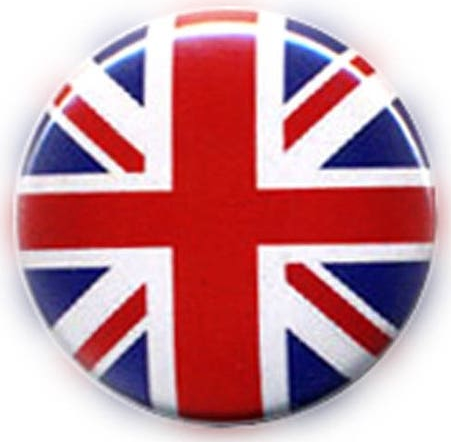
\includegraphics[scale=0.12]{english}}\  In English \raisebox{-2.5pt}{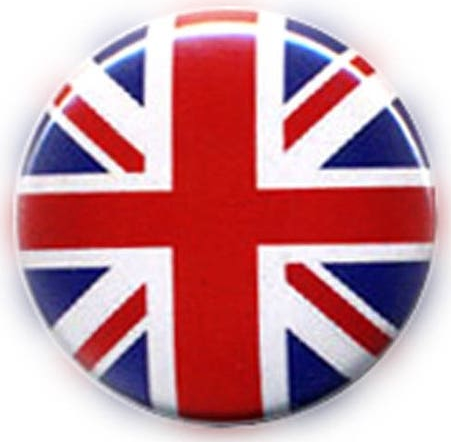
\includegraphics[scale=0.12]{english}}\ : #1}

\newcommand{\voir}[1]{\textcolor{purple}{\faBook\ voir #1}}

\newcommand{\exoschoisis}[1]{\faBook\ Exercices associés~:\ #1}

\newcommand{\augustin}[1]{
\includegraphics[width=#1\linewidth]{Logo_augustin_thierry}}
\newcommand{\acad}[1]{
\includegraphics[width=#1\linewidth]{logo_acad}}

\newcommand{\geogebra}[1]{\href{#1}{\raisebox{-0.35em}{
\includegraphics[scale=0.3]{geogebra}}\ #1\ \raisebox{-0.35em}{
\includegraphics[scale=0.3]{geogebra}}}}

\newcommand{\activite}[2][]{\textcolor{purple}{\faBook\ Activité#1 d'introduction : Situation#1 #2}}


%%%%%%%%%%%%%%%%%%%%%%%%%%%%%%%%%%%%%%%%%%%%%%%%%%%%%%%%%%%%%%
%%%%%%%%%%%%%%%%%%%%%%%%%%%%%%%%%%%%%%%%%%%%%%%%%%%%%%%%%%%%%%


%___________________________
%===    HYPERLIENS
%------------------------------------------------------
\usepackage[colorlinks=true,linkcolor=black,filecolor=blue,urlcolor=blue,bookmarksnumbered]{hyperref} 
%%%%%%%%%%%%%%%%%%%%%%%%%%%%%%%%%%%%%%%%%%%%%%%%%%%%%%%%%%%%%%%%%%%%%%%%%%%%%%%
\portrait
%entête classique

\fancypagestyle{garde_tete}{% 
\fancyhead[C]{\small\textbf{Ti\textit{k}Z} \hfill \small \textbf{Année 2013-2014}}
\renewcommand{\headrulewidth}{0cm}}

\newcommand{\tete}{
\thispagestyle{garde_tete}
\begin{tikzpicture}
\node[shading=ball,ball color=OliveGreen,rectangle,draw=black,rounded corners,thick]{%
\begin{minipage}{\linewidth}
\begin{center}
\vspace*{9pt}
\Large \textsc{\textbf{Exemples de graphiques avec Ti\textit{k}Z}}
\vspace*{9pt}
\end{center}
\end{minipage}
};\end{tikzpicture}

\noindent 
\vspace{-6pt}
}

%%%%%%%%%%%%%%%%%%%%%%%%%%%%%%%%%%%%%%%%%%%%%%%%%%%%%%%%%%%%%%%%%%%%%%%%%%%%%%%
%Pour l'exercice 1

% commande pour la version améliorée de Tikz (section 3)
\newcommand{\Noeud}[2]{%
    \tikz[remember picture]{\node[inner sep=0pt,outer sep=4pt](#1){#2};}
}

% "outer sep" pour la distance de la flèche par rapport au point.
% j'interprète "inner sep" comme étant la taille du noeud. En mettant cette taille à 0pt, le noeud reste sur la ligne et cela évite l'utilisation de \raisebox
% La commande n'a qu'un seul argument.
% Le nom du noeud est écrit entre parenthèse et n'apparaît pas dans le texte. Mais c'est ce nom là qui est utilisé pour les calculs des dimensions des "boîtes" par LaTeX.
% Le nom spécifié entre accolades est le texte qui apparaîtra pour de vrai. Pour nos besoins, ce nom est du texte mathématiques et correspond au nom du noeud.
%
% Les noms spécifiés dans un environnement Tikz ne servent que pour la figure en cours.
% L'option "remember picture" permet de sauvegarder le nom des noeuds qui seront utilisés dans d'autres figures (ici, les figures pour dessiner les flèches).

\tikzset{Perso/.style={line cap=round,line join=round, line width=1pt,>=stealth}} % permet d'écrire Perso dans les commandes tikz pour éviter de tout écrire et tout modifier si nécessaire.

%%%%%%%%%%%%%%%%%%%%%%%%%%%%%%%%%%%%%%%%%%%%%%%%%%%%%%%%%%%%%%%%%%%%%%%%%%%%%%%

%%%%%%%%%%%%%%%%%%%%%%%
%% DEBUT DU DOCUMENT %%
%%%%%%%%%%%%%%%%%%%%%%%

\begin{document}

\setlength\parindent{0mm}
\tete 		%entête classique


\renewcommand \footrulewidth{0.2pt}%
\renewcommand \headrulewidth{0pt}%
\pagestyle{fancy}
\fancyhf{}
\pieddepage{Ti\textit{k}Z}{\thepage / \pageref{LastPage}}{Année 2017-2018}


%%%%%%%%%%%%%%%%%%%%%%%Page 1%%%%%%%%%%%%%%%%%%%%%%%%%%%%%%%%%%%%%%%%
\begin{spacing}{1.2}
%%%%%%%%%%%%%%%%%%%%%%%%%%%%%%%%%%%%%%%%%%%%%%%%%%%%%%%%%%%%
\begin{Exercice}[]
\label{exo1}

\textbf{Avec Pstricks : version Philippe année 2007}

{\small

\[\rnode{K}{k} \times (\rnode{A}{a}+\rnode{B}{b}) = \textcolor{red}{k\times a}+\textcolor{blue}{k\times b}\]
\ncarc[linecolor=red,arcangle=90]{->}{K}{A}
\ncarc[linecolor=blue,arcangle=-90]{->}{K}{B}


Voici la formule de la distributivité :
$\rnode{K}{k} \times (\rnode{A}{a}+\rnode{B}{b}) = \textcolor{red}{k\times a}+\textcolor{blue}{k\times b}$
\ncarc[linecolor=red,arcangle=90]{->}{K}{A}
\ncarc[linecolor=blue,arcangle=-90]{->}{K}{B}
vue en 5\ieme.\bigskip


\[(\rnode{A}{a}+\rnode{B}{b})\times(\rnode{C}{c}+\rnode{D}{d})=\textcolor{red}{a\times c}+\textcolor{blue}{a\times d}+b\times c+\textcolor{Peach}{b\times d}\]
\ncarc[linecolor=red,arcangle=90]{->}{A}{C}
\ncarc[linecolor=blue,arcangle=90]{->}{A}{D}
\ncarc[arcangle=-90]{->}{B}{C}
\ncarc[linecolor=Peach,arcangle=-90]{->}{B}{D}

Voici la formule de la distributivité :
$(\rnode{A}{a}+\rnode{B}{b})\times(\rnode{C}{c}+\rnode{D}{d})=\textcolor{red}{a\times c}+\textcolor{blue}{a\times d}+b\times c+\textcolor{Peach}{b\times d}$
\ncarc[linecolor=red,arcangle=90]{->}{A}{C}
\ncarc[linecolor=blue,arcangle=90]{->}{A}{D}
\ncarc[arcangle=-90]{->}{B}{C}
\ncarc[linecolor=Peach,arcangle=-90]{->}{B}{D}
vue en 4\ieme.
}

\textbf{Avec Tikz : version Dominique}

\begin{center}
\begin{tikzpicture}[scale=1,x=1.0cm]
\draw (0,0) node [right] {$a\times (b+c)=\textcolor{blue}{a\times b}+\textcolor{red}{a\times c}$};
\draw[Perso,->,color=blue](0.25,0.25) to[bend left] (1,0.25);
\draw[Perso,->,color=red](0.25,0.25) to[bend left] (1.7,0.25);
\end{tikzpicture}
\end{center}

\begin{center}
\begin{tikzpicture}[scale=1,x=1.0cm]
\draw (0,0) node [right] {$(a+b)\times (c+d)=\textcolor{blue}{a\times c}+\textcolor{blue}{a\times d}+\textcolor{red}{b\times c}+\textcolor{red}{b\times d}$};
\draw[Perso,->,color=blue](0.4,0.25) to[bend left] (1.9,0.25);
\draw[Perso,->,color=blue](0.4,0.25) to[bend left] (2.5,0.25);
\draw[Perso,->,color=red](1,-0.25) to[bend right] (1.9,-0.25);
\draw[Perso,->,color=red](1,-0.25) to[bend right] (2.5,-0.25);
\end{tikzpicture}
\end{center}

%%%%%%%%%%%%%%%%%%%%%%%%%%%%%%%%%%%%%%%%%%%%%%%%%%%%%%%%%%%%
\begin{center}
Au milieu d'un texte :
\end{center}
Voici la formule de la simple distributivité :
\raisebox{-4pt}{
\begin{tikzpicture}[scale=1,x=1.0cm]
\draw (0,0) node [right] {$a\times (b+c)=\textcolor{blue}{a\times b}+\textcolor{red}{a\times c}$};
\draw[Perso,->,color=blue](0.25,0.25) to[bend left] (1,0.25);
\draw[Perso,->,color=red](0.25,0.25) to[bend left] (1.7,0.25);
\end{tikzpicture}}
(vue en 5\up{ème}).

Voici la formule de la double distributivité :
\raisebox{-12pt}{
\begin{tikzpicture}[scale=1,x=1.0cm]
\draw (0,0) node [right] {$(a+b)\times (c+d)=\textcolor{blue}{a\times c}+\textcolor{blue}{a\times d}+\textcolor{red}{b\times c}+\textcolor{red}{b\times d}$};
\draw[Perso,->,color=blue](0.4,0.25) to[bend left] (1.9,0.25);
\draw[Perso,->,color=blue](0.4,0.25) to[bend left] (2.5,0.25);
\draw[Perso,->,color=red](1,-0.25) to[bend right] (1.9,-0.25);
\draw[Perso,->,color=red](1,-0.25) to[bend right] (2.5,-0.25);
\end{tikzpicture}}
(vue en 4\up{ème}).

\textbf{Avec Tikz : version améliorée}

{\small

\[\Noeud{a}{a} \times (\Noeud{b}{b}+\Noeud{c}{c}) = \textcolor{blue}{a\times b}+\textcolor{red}{a\times c}\]
% pour tracer les flèches :
\begin{tikzpicture}[remember picture,overlay,>=stealth]
    \draw[Perso,->,blue] (a.south) to[out=-75,in=-120,distance=0.25cm]  (b.south);
    \draw[Perso,->,red] (a.north) to[bend left=50]  (c.north);
\end{tikzpicture}

% on spécifie d'où par la flèche et d'où elle arrive en nommant le noeud.
% chaque noeud est encadré par un rectangle et on peut accéder à des points particulier avec les commandes .north, .south, .west, .east.
% on peut être plus précis en écrivant .18 qui est l'angle en degré par rapport à l'horizontal et dans le sens trigonométrique
%
% la commande distance=0.25cm permet de gérer la distance de la courbure de la flèche. Faîtes des tests pour mieux comprendre.
%
% la commande bend left (ou bend right) permet de courber la courbe dans un sens ou dans l'autre.
% pour bend left, la courbure est placée à gauche du chemin en ligne droite dans le sens du parcours.
% le nombre indiqué est l'angle par rapport à l'horizontal au point de départ et à celui d'arrivée.
%
% pour être plus précis, on peut spécifier l'angle au départ : out=50 et celui à l'arrivée : in=120 (toujours en degré, par rapport à l'horizontal dans le sens trigo)

\[(\Noeud{a}{a} + \Noeud{b}{b}) \times (\Noeud{c}{c} + \Noeud{d}{d}) = \textcolor{blue}{a\times c}+\textcolor{blue}{a\times d}+\textcolor{red}{b\times c}+\textcolor{red}{b\times d}\]
% pour tracer les flèches :
\begin{tikzpicture}[remember picture,overlay,>=stealth]
    \draw[Perso,->,blue] (a.north) to[bend left = 50]  (c.north);
    \draw[Perso,->,blue] (a.north) to[bend left=50]  (d.north);
    \draw[Perso,->,red] (b.south) to[bend right = 50]  (c.south);
    \draw[Perso,->,red] (b.south) to[bend right= 50]  (d.south);
\end{tikzpicture}

\begin{center}
    Au milieu d'un texte :
\end{center}


Voici la formule de la simple distributivité : $\Noeud{a}{a} \times (\Noeud{b}{b}+\Noeud{c}{c}) = \textcolor{blue}{a\times b}+\textcolor{red}{a\times c}$ (vue en 5\up{ème}).\vspace{1cm}
% pour tracer les flèches :
\begin{tikzpicture}[remember picture,overlay,>=stealth]
    \draw[Perso,->,blue] (a.south) to[out=-75,in=-120,distance=0.25cm]  (b.south);
    \draw[Perso,->,red] (a.north) to[bend left=50]  (c.north);
\end{tikzpicture}

Voici la formule de la double distributivité : $(\Noeud{a}{a} + \Noeud{b}{b}) \times (\Noeud{c}{c} + \Noeud{d}{d}) = \textcolor{blue}{a\times c}+\textcolor{blue}{a\times d}+\textcolor{red}{b\times c}+\textcolor{red}{b\times d}$ (vue en 4\up{ème}).
% pour tracer les flèches :
\begin{tikzpicture}[remember picture,overlay,>=stealth]
    \draw[Perso,->,blue] (a.north) to[bend left = 50]  (c.north);
    \draw[Perso,->,blue] (a.north) to[bend left=50]  (d.north);
    \draw[Perso,->,red] (b.south) to[bend right = 50]  (c.south);
    \draw[Perso,->,red] (b.south) to[bend right= 50]  (d.south);
\end{tikzpicture}
}

\setlength{\columnseprule}{0pt}
\begin{multicols}{3}\raggedcolumns
\begin{center}
Son graphique est\dots
\vspace*{2em}

\begin{flushright}
\dots une droite \Noeud{1}{$\Box$} \hspace*{2em}

\dots une parabole \Noeud{2}{$\Box$} \hspace*{2em}

\dots une hyperbole \Noeud{3}{$\Box$} \hspace*{2em}

\dots d'un autre type \Noeud{4}{$\Box$} \hspace*{2em}
\end{flushright}
\end{center}
\columnbreak
\begin{center}
Expressions des fonctions :

\bigskip

\hspace*{1em}\Noeud{5}{$\Box$} \hfill $f(x)=5$\hfill \Noeud{11}{$\Box$}\hspace*{1em}

\hspace*{1em}\Noeud{6}{$\Box$} \hfill $g(x)=x+4$\hfill \Noeud{12}{$\Box$}\hspace*{1em}

\hspace*{1em}\Noeud{7}{$\Box$} \hfill $h(x)=\dfrac{1}{3}x+\dfrac{1}{2}$\hfill \Noeud{13}{$\Box$}\hspace*{1em}

\hspace*{1em}\Noeud{8}{$\Box$} \hfill $k(x)=x^2$\hfill \Noeud{14}{$\Box$}\hspace*{1em}
\\[0.5em]
\hspace*{1em}\Noeud{9}{$\Box$} \hfill $l(x)=\dfrac{1}{x}$\hfill \Noeud{15}{$\Box$}\hspace*{1em}
\\[0.5em]
\hspace*{1em}\Noeud{10}{$\Box$} \hfill $m(x)=\sqrt{x}$\hfill \Noeud{16}{$\Box$}\hspace*{1em}
\end{center}
\columnbreak

\begin{center}
C'est\dots
\vspace*{2em}

\begin{flushleft}
\hspace*{2em} \Noeud{17}{$\Box$} \dots une fonction affine

\hspace*{2em} \Noeud{18}{$\Box$} \dots la fonction carré

\hspace*{2em} \Noeud{19}{$\Box$} \dots la fonction inverse

\hspace*{2em} \Noeud{20}{$\Box$} \dots une autre fonction
\end{flushleft}
\end{center}

\end{multicols}

\begin{tikzpicture}[remember picture,overlay,color=blue,line width=1.5pt]
\draw(1.center)--(5.center);
\draw(1.center)--(6.center);
\draw(1.center)--(7.center);
\draw(2.center)--(8.center);
\draw(3.center)--(9.center);
\draw(4.center)--(10.center);
\draw(11.center)--(17.center);
\draw(12.center)--(17.center);
\draw(13.center)--(17.center);
\draw(14.center)--(18.center);
\draw(15.center)--(19.center);
\draw(16.center)--(20.center);
\end{tikzpicture}

\end{Exercice}
%%%%%%%%%%%%%%%%%%%%%%%%%%%%%%%%%%%%%%%%%%%%%%%%%%%%%%%%%%%%
%\newpage
\medskip
\begin{Exercice}[Graphes probabilistes]
\label{exo2}


\begin{center}
\begin{tikzpicture}[scale=1]
\tikzstyle{every path}=[line width=1pt];
\node [draw,circle,fill=gray!50] (A) at (0,0) {A};
\node [draw,circle,fill=gray!50] (B) at (4,0) {B};
\draw (A) to [bend left]  node[midway,sloped,above] {$0,9$} node[midway,sloped]{>} (B);
\draw (B) to [bend left] node[midway,sloped,below] {$0,7$} node [midway,sloped] {<} (A);
\draw (B) .. controls +(1.5,-1) and +(1.5,1) .. node[midway,right]{$0,3$} node [midway,sloped] {>} (B) ;
\draw (A) .. controls +(-1.5,-1) and +(-1.5,1) .. node[midway,left]{$0,1$} node [midway,sloped] {>} (A) ;
\end{tikzpicture}
\end{center}

\begin{center}
\begin{tikzpicture}[scale=1]
\tikzstyle{every path}=[>=stealth,->,line width=1pt];
\node [draw,circle,fill=gray!50] (A) at (0,0) {A};
\node [draw,circle,fill=gray!50] (B) at (4,0) {B};
\draw[->] (A) to [bend left]  node[midway,sloped,above] {\dots}(B);
\draw[->] (B) to [bend left] node[midway,sloped,above] {\dots} (A);
\draw[->] (B) .. controls +(1.5,-1) and +(1.5,1) .. node[midway,right]{\dots} (B) ;
\draw[->] (A) .. controls +(-1.5,-1) and +(-1.5,1) .. node[midway,left]{\dots} (A) ;
\end{tikzpicture}
\end{center}

\begin{center}
\begin{tikzpicture}[scale=1]
\tikzstyle{every path}=[>=stealth,->,line width=1pt];
\node [draw,circle,fill=gray!50] (A) at (0,0) {1};
\node [draw,circle,fill=gray!50] (B) at (4,0) {2};
\node [draw,circle,fill=gray!50] (C) at (2,-3) {3};
\draw[->] (A) to [out=20,in=160]  node[midway,sloped,above] {$0,3$}(B);
\draw[->] (A) to [out=-40,in=115]  node[midway,sloped,above] {$0,2$}(C);
\draw[->] (B) to [out=-160,in=-20] node[midway,sloped,above] {$0,3$} (A);
\draw[->] (B) to [out=-140,in=75] node[midway,sloped,above] {$0,3$} (C);
\draw[->] (C) to [out=150,in=-90] node[midway,sloped,above] {$0,2$} (A);
\draw[->] (C) to [out=30,in=-90] node[midway,sloped,above] {$0,3$} (B);
\draw[->] (B) .. controls +(1.5,-1) and +(1.5,1) .. node[midway,right]{$0,4$} (B) ;
\draw[->] (A) .. controls +(-1.5,-1) and +(-1.5,1) .. node[midway,left]{$0,5$} (A) ;
\draw[->] (C) .. controls +(-1,-1.5) and +(1,-1.5) .. node[midway,below]{$0,5$} (C) ;
\end{tikzpicture}
\end{center}


\end{Exercice}

%%%%%%%%%%%%%%%%%%%%%%%%%%%%%%%%%%%%%%%%%%%%%%%%%%%%%%%%%%%%

\begin{Exercice}[]
\label{exo3}
\begin{tikzpicture}[x={(1cm,0cm)},y={(0.5cm,1cm)}]    
    \draw[color=black,line width=1.5pt](-1,0)--(5,0);
    \draw[color=black,line width=1.5pt](0,-1)--(0,5);
    \draw (0,0) node [above left] {A};
    \draw (1,-12pt) node {I};
    \draw[line width=1.5pt](1,0) -- ++(0pt,3pt)-- ++(0pt,-6pt);
    \draw (0,1) node [above left] {J};
    \draw[line width=1.5pt](0,1) -- ++(-2pt,2pt) -- ++(4pt,-4pt);
\end{tikzpicture}

\end{Exercice}
%%%%%%%%%%%%%%%%%%%%%%%%%%%%%%%%%%%%%%%%%%%%%%%%%%%%%%%%%%%%

\begin{Exercice}[]\label{exo4}

\begin{center}
\begin{tikzpicture}
    	\tkzTabInit[nocadre]{$x$/1,Signe de \\ $3x$/1.5,Signe de \\ $x-2$/1.5, Signe de \\ $3x(x-2)$/1.5}{$-\infty$,$0$,$2$,$+\infty$}
        \tkzTabLine{,-,z,,+,}
        \tkzTabLine{,,-,,z,+,}
        \tkzTabLine{,+,z,-,z,+,}
\end{tikzpicture}
\end{center}

\begin{center}
\begin{tikzpicture}
    	\tkzTabInit[lgt=3]{$x$/1,Signe de \\ $3x$/1.5,Signe de \\ $x-2$/1.5, Signe de \\ $3x(x-2)$/1.5,Variations de \\$f$ /3}{$-\infty$,$0$,$2$,$+\infty$}
        \tkzTabLine{,-,z,,+,}
        \tkzTabLine{,,-,,z,+,}
        \tkzTabLine{,+,z,-,z,+,}
        \tkzTabVar{+/$+\infty$,-/$-\dfrac{1}{2}$,+/$\dfrac{17}{128}$,-/$-\infty$}
	\end{tikzpicture}
\end{center}

\end{Exercice}
%%%%%%%%%%%%%%%%%%%%%%%%%%%%%%%%%%%%%%%%%%%%%%%%%%%%%%%%%%%%
\vspace*{12pt}
\[\star\star\star\star\star\star\star\star\star\star\star\star\star\star\star\star\]
\vspace*{12pt}
%%%%%%%%%%%%%%%%%%%%%%%%%%%%%%%%%%%%%%%%%%%%%%%%%%%%%%%%%%%%
\begin{Exercice}[]\label{exo5}

\begin{center}
\begin{tikzpicture}[scale=1,line cap=round,line join=round,x=1.0cm]
\draw[>=stealth,->,line width=1.5pt,color=blue] (-5.5,0) -- (5.5,0);
\draw[{]-]},line width=3pt,color=red] (-2.5,0) -- (3,0);
\foreach \x in {-5,...,5}{
\draw[color=black,line width=1.5pt] (\x,2pt) -- (\x,-2pt);}
\foreach \x in {-5,...,5}{
\draw (\x,-7pt) node[below,font=\bfseries] {\x};}
\end{tikzpicture}
\end{center}

\end{Exercice}
%%%%%%%%%%%%%%%%%%%%%%%%%%%%%%%%%%%%%%%%%%%%%%%%%%%%%%%%%%%%

\begin{Exercice}[]\label{exo6}

\textbf{Segments définis avec les lettres}

\begin{center}
\begin{tikzpicture}[scale=1,line cap=round,line join=round,>=stealth,x=1.0cm,y=1.0cm]
\coordinate (A) at (0,0);\node [font=\bfseries,color=blue,below left] at (A) {A};
\coordinate (B) at (5,0);\node [font=\bfseries,color=blue,below right] at (B) {B};
\coordinate (C) at (5,3);\node [font=\bfseries,color=blue,above right] at (C) {C};
\coordinate (D) at (0,3);\node [font=\bfseries,color=blue,above left] at (D) {D};
\coordinate (M) at (2,0);\node [font=\bfseries,color=OliveGreen,below right] at (M) {M};
\coordinate (N) at (5,2);\node [font=\bfseries,color=OliveGreen,above right] at (N) {N};
\coordinate (P) at (3,3);\node [font=\bfseries,color=OliveGreen,above left] at (P) {P};
\coordinate (Q) at (0,1);\node [font=\bfseries,color=OliveGreen,above left] at (Q) {Q};
\draw [color=black, line width=1pt,fill=pink!50] (A)--(B)--(C)--(D)--cycle;
\draw [color=black, line width=1.5pt] (A)--(M) node[midway,sloped] {||};
\draw [color=black, line width=1.5pt] (B)--(N) node[midway,sloped] {||};
\draw [color=black, line width=1.5pt] (C)--(P) node[midway,sloped] {||};
\draw [color=black, line width=1.5pt] (D)--(Q) node[midway,sloped] {||};
\draw [color=red, line width=1pt,fill=pink] (M)--(N)--(P)--(Q)--cycle;
\draw [line width=1.5pt] (M)-- ++(3pt,3pt)-- ++(-6pt,-6pt)-- ++(3pt,3pt)-- ++(-3pt,3pt)-- ++(6pt,-6pt);
\draw [line width=1.5pt] (N)-- ++(3pt,3pt)-- ++(-6pt,-6pt)-- ++(3pt,3pt)-- ++(-3pt,3pt)-- ++(6pt,-6pt);
\draw [line width=1.5pt] (P)-- ++(3pt,3pt)-- ++(-6pt,-6pt)-- ++(3pt,3pt)-- ++(-3pt,3pt)-- ++(6pt,-6pt);
\draw [line width=1.5pt] (Q)-- ++(3pt,3pt)-- ++(-6pt,-6pt)-- ++(3pt,3pt)-- ++(-3pt,3pt)-- ++(6pt,-6pt);
\end{tikzpicture}
\end{center}

\end{Exercice}

%%%%%%%%%%%%%%%%%%%%%%%%%%%%%%%%%%%%%%%%%%%%%%%%%%%%%%%%%%%%

\begin{Exercice}[]\label{exo7}

\begin{center}
\begin{tikzpicture}[scale=1,line cap=round,line join=round,>=stealth,x=1.0cm,y=1.0cm]
\draw [color=gray!50, xstep=0.5,ystep=0.5] (-5.5,-5.5) grid (5.5,5.5);
\draw[->,line width=1.5pt,color=blue] (-5.5,0) -- (5.5,0);
\foreach \x in {-5,...,5}{
\draw[color=black] (\x,2pt) -- (\x,-2pt) node[below,font=\bfseries] {\x};}
\draw[->,line width=1.5pt,color=blue] (0,-5.5) -- (0,5.5);
\foreach \y in {-5,...,5}{
\draw[color=black] (2pt,\y) -- (-2pt,\y) node[left,font=\bfseries] {\y};}
%\draw[color=black] (0pt,0pt) node[below left] {\footnotesize $0$};%%%%%%%%%%%marque 0 à l'origine, en bas, à gauche
\clip(-5.5,-5.5) rectangle (5.5,5.5);%%%%%%%%%%%%réduit la fenêtre d'affichage de ce qui suit
\draw[smooth,samples=200,domain=-5.5:5,line width=2pt,color=red] plot(\x,{-5+exp(\x)});
\end{tikzpicture}
\end{center}

\end{Exercice}

%%%%%%%%%%%%%%%%%%%%%%%%%%%%%%%%%%%%%%%%%%%%%%%%%%%%%%%%%%%%

\begin{Exercice}[]\label{exo8}

\begin{center}
\begin{tikzpicture}[scale=1,line cap=round,line join=round,>=stealth,x=0.2cm,y=1.0cm]
\draw [color=gray!75, xstep=5,ystep=0.5] (80,-1) grid (150,4);
\draw[->,line width=2pt,color=blue] (80,0) -- (150,0);
\foreach \x in {90,100,110,120,130,140}{
\draw[color=black,line width=1.5pt] (\x,2pt) -- (\x,-2pt) node[below,font=\bfseries] {\x};}
\draw [color=blue, line width=2pt](89,1)--(89,3);
\draw [color=blue, line width=2pt](89,2)--(103,2);
\draw [color=blue, line width=2pt](103,1)--(103,3)--(121,3)--(121,1)--cycle;
\draw [color=blue, line width=2pt](121,2)--(139,2);
\draw [color=blue, line width=2pt](139,1)--(139,3);
\draw [color=red, line width=2pt](110,1)--(110,3);
\end{tikzpicture}
\end{center}

\end{Exercice}

%%%%%%%%%%%%%%%%%%%%%%%%%%%%%%%%%%%%%%%%%%%%%%%%%%%%%%%%%%%%

\begin{Exercice}[]\label{exo9}

\begin{center}
\begin{tikzpicture}[scale=1,line cap=round,line join=round,>=stealth,x=1.0cm,y=1.0cm]
\clip(0,0) circle (2);%%%%%%%%%%%%réduit la fenêtre d'affichage de ce qui suit
\draw [color=gray!50, xstep=0.5,ystep=0.5] (-5.5,-5.5) grid (5.5,5.5);
\draw[->,line width=1.5pt,color=blue] (-5.5,0) -- (5.5,0);
\foreach \x in {-5,...,5}{
\draw[color=black] (\x,2pt) -- (\x,-2pt) node[below,font=\bfseries] {\x};}
\draw[->,line width=1.5pt,color=blue] (0,-5.5) -- (0,5.5);
\foreach \y in {-5,...,5}{
\draw[color=black] (2pt,\y) -- (-2pt,\y) node[left,font=\bfseries] {\y};}
%\draw[color=black] (0pt,0pt) node[below left] {\footnotesize $0$};%%%%%%%%%%%marque 0 à l'origine, en bas, à gauche
\draw[smooth,samples=200,domain=-5:5,line width=2pt,color=red] plot(\x,{-5+exp(\x)});
\end{tikzpicture}
\end{center}

\end{Exercice}

%%%%%%%%%%%%%%%%%%%%%%%%%%%%%%%%%%%%%%%%%%%%%%%%%%%%%%%%%%%%
%%%%%%%%%%%%%%%%%%%%%%%%%%%%%%%%%%%%%%%%%%%%%%%%%%%%%%%%%%%%

\begin{Exercice}[]\label{exo10}
\begin{center}
\begin{tikzpicture}[scale=1,line cap=round,line join=round,>=stealth,x=1.0cm,y=1.0cm]
\draw [color=gray!50, xstep=0.5,ystep=0.5] (-5.5,-5.5) grid (5.5,5.5);
\draw [color=gray!, xstep=1,ystep=1,line width=1.5pt] (-5.5,-5.5) grid (5.5,5.5);
\draw[->,line width=1.5pt,color=blue] (-5.5,0) -- (5.5,0);
\foreach \x in {-5,...,5}{
\draw[color=black] (\x,2pt) -- (\x,-2pt) node[below,font=\bfseries] {\x};}
\draw[->,line width=1.5pt,color=blue] (0,-5.5) -- (0,5.5);
\foreach \y in {-5,...,5}{
\draw[color=black] (2pt,\y) -- (-2pt,\y) node[left,font=\bfseries] {\y};}
%\draw[color=black] (0pt,0pt) node[below left] {\footnotesize $0$};%%%%%%%%%%%marque 0 à l'origine, en bas, à gauche
\clip(-5,-5) rectangle (5.5,5.5);%%%%%%%%%%%%réduit la fenêtre d'affichage de ce qui suit
\draw[smooth,samples=200,domain=-5:5,line width=2pt,color=red] plot(\x,{-5+exp(\x)});
\end{tikzpicture}
\end{center}

\end{Exercice}


%%%%%%%%%%%%%%%%%%%%%%%%%%%%%%%%%%%%%%%%%%%%%%%%%%%%%%%%%%%%
%%%%%%%%%%%%%%%%%%%%%%%%%%%%%%%%%%%%%%%%%%%%%%%%%%%%%%%%%%%%

\begin{Exercice}[]\label{exo11}

\begin{center}
\begin{tikzpicture}[scale=0.15,line cap=round,line join=round,>=stealth,x=1.0cm,y=1.0cm]
\draw [color=gray!50, xstep=5,ystep=5] (-55,-55) grid (55,55);
\draw [color=gray!, xstep=10,ystep=10,line width=1.5pt] (-55,-55) grid (55,55);
\draw[->,line width=1.5pt,color=blue] (-55,0) -- (55,0);
\foreach \x in {-55,-50,-45,-40,-35,-30,-25,-20,-15,-10,-5,5,10,15,20,25,30,35,40,45,50}{
\draw[color=black] (\x,2pt) -- (\x,-2pt) node[below] {\footnotesize $\x$};}
\draw[->,line width=1.5pt,color=blue] (0,-55) -- (0,55);
\foreach \y in {-55,-50,-45,-40,-35,-30,-25,-20,-15,-10,-5,5,10,15,20,25,30,35,40,45,50}{
\draw[color=black] (2pt,\y) -- (-2pt,\y) node[left] {\footnotesize $\y$};}
\draw[color=black] (0pt,0pt) node[below left] {\footnotesize $0$};%%%%%%%%%%%marque 0 à l'origine, en bas, à gauche
%\clip(-5,-5) rectangle (5.5,5.5);%%%%%%%%%%%%réduit la fenêtre d'affichage de ce qui suit
\draw[smooth,samples=200,domain=-30:40,line width=2pt,color=red] plot(\x,{50*sin(50*\x)});
\end{tikzpicture}
\end{center}

\end{Exercice}

%%%%%%%%%%%%%%%%%%%%%%%%%%%%%%%%%%%%%%%%%%%%%%%%%%%%%%%%%%%%
%%%%%%%%%%%%%%%%%%%%%%%%%%%%%%%%%%%%%%%%%%%%%%%%%%%%%%%%%%%%

\begin{Exercice}[]\label{exo12}

\begin{center}
\begin{tikzpicture}[scale=1,line cap=round,line join=round,>=stealth,x=0.15cm,y=0.15cm]
\draw [color=gray!50, xstep=5,ystep=5] (-55,-55) grid (55,55);
\draw [color=gray!, xstep=10,ystep=10,line width=1.5pt] (-55,-55) grid (55,55);
\draw[->,line width=1.5pt,color=blue] (-55,0) -- (55,0);
\foreach \x in {-55,-50,-45,-40,-35,-30,-25,-20,-15,-10,-5,5,10,15,20,25,30,35,40,45,50}{
\draw[color=black] (\x,2pt) -- (\x,-2pt) node[below] {\footnotesize $\x$};}
\draw[->,line width=1.5pt,color=blue] (0,-55) -- (0,55);
\foreach \y in {-55,-50,-45,-40,-35,-30,-25,-20,-15,-10,-5,5,10,15,20,25,30,35,40,45,50}{
\draw[color=black] (2pt,\y) -- (-2pt,\y) node[left] {\footnotesize $\y$};}
\draw[color=black] (0pt,0pt) node[below left] {\footnotesize $0$};%%%%%%%%%%%marque 0 à l'origine, en bas, à gauche
%\clip(-5,-5) rectangle (5.5,5.5);%%%%%%%%%%%%réduit la fenêtre d'affichage de ce qui suit
\draw[smooth,samples=200,domain=-30:40,line width=2pt,color=red] plot(\x,{50*sin(50*\x)});
\end{tikzpicture}
\end{center}

\end{Exercice}

%%%%%%%%%%%%%%%%%%%%%%%%%%%%%%%%%%%%%%%%%%%%%%%%%%%%%%%%%%%%
%%%%%%%%%%%%%%%%%%%%%%%%%%%%%%%%%%%%%%%%%%%%%%%%%%%%%%%%%%%%

\begin{Exercice}[]\label{exo13}

\begin{center}
\begin{tikzpicture}[scale=1,line cap=round,line join=round,>=stealth,x=0.02cm,y=0.1cm]
\draw [color=gray!50, xstep=25,ystep=5] (0,0) grid (510,105);
\draw [color=gray!, xstep=50,ystep=10,line width=1.5pt] (0,0) grid (510,105);
\draw[->,line width=1.5pt,color=blue] (-25,0) -- (510,0);
\foreach \x in {50,100,150,200,250,300,350,400,450,500}{
\draw[color=black] (\x,2pt) -- (\x,-2pt) node[below] {\footnotesize $\x$};}
\draw[->,line width=1.5pt,color=blue] (0,-5) -- (0,105);
\foreach \y in {10,20,30,40,50,60,70,80,90,100}{
\draw[color=black] (2pt,\y) -- (-2pt,\y) node[left] {\footnotesize $\y$};}
\draw[color=black] (0pt,0pt) node[below left] {\footnotesize $0$};%%%%%%%%%%%marque 0 à l'origine, en bas, à gauche
%\clip(-5,-5) rectangle (5.5,5.5);%%%%%%%%%%%%réduit la fenêtre d'affichage de ce qui suit
\draw[smooth,samples=200,domain=0:500,line width=2pt,color=red] plot(\x,{100/(\x+1)});
\end{tikzpicture}
\end{center}

\end{Exercice}

%%%%%%%%%%%%%%%%%%%%%%%%%%%%%%%%%%%%%%%%%%%%%%%%%%%%%%%%%%%%
%%%%%%%%%%%%%%%%%%%%%%%%%%%%%%%%%%%%%%%%%%%%%%%%%%%%%%%%%%%%

\begin{Exercice}[]\label{exo14}

\begin{center}
\begin{tikzpicture}[scale=1.1,line cap=round,line join=round,>=stealth,x=0.015cm,y=0.075cm]
\draw [color=gray!50, xstep=25,ystep=5] (0,0) grid (1000,100);
\draw [color=gray!, xstep=50,ystep=10,line width=1.5pt] (0,0) grid (1000,100);
\draw[->,line width=1.5pt,color=blue] (0,0) -- (1000,0);
\foreach \x in {0,50,100,150,200,250,300,350,400,450,500,550,600,650,700,750,800,850,900,950}{
\draw[color=black] (\x,2pt) -- (\x,-2pt) node[below] {\footnotesize $\x$};}
\draw[->,line width=1.5pt,color=blue] (0,0) -- (0,100);
\foreach \y in {0,10,20,30,40,50,60,70,80,90}{
\draw[color=black] (2pt,\y) -- (-2pt,\y) node[left] {\footnotesize $\y$};}
%\draw[color=black] (0pt,0pt) node[below left] {\footnotesize $0$};%%%%%%%%%%%marque 0 à l'origine, en bas, à gauche
\clip(0,0) rectangle (1000,98);%%%%%%%%%%%%réduit la fenêtre d'affichage de ce qui suit
\draw[smooth,samples=200,domain=0:1000,line width=2pt,color=red] plot(\x,{89.5-8.9*ln(\x+0.3)});
\end{tikzpicture}
\end{center}

\end{Exercice}

%%%%%%%%%%%%%%%%%%%%%%%%%%%%%%%%%%%%%%%%%%%%%%%%%%%%%%%%%%%%

\begin{Exercice}[]\label{exo15}

\begin{center}
\begin{tikzpicture}[scale=2,line cap=round,line join=round,>=stealth,x=1.0cm,y=1.0cm]
\foreach \x in {-2,...,2}{
\draw[color=black] (\x,2pt) -- (\x,-2pt) node[below right] {$\x$};}
\foreach \y in {-1,...,2}{
\draw[color=black] (2pt,\y) -- (-2pt,\y) node[above left] {$\y$};}
\clip(-2.5,-1) rectangle (2.5,3);%%%%%%%%%%%%réduit la fenêtre d'affichage de ce qui suit
\draw[smooth,samples=200,domain=-2.5:2.5,line width=2pt,color=red] plot(\x,{(2-\x)*exp(\x)});
\draw(1.5,2) node[below left] {$\mathcal{C}$};
\draw[smooth,samples=200,domain=-2.5:2.5,line width=2pt,color=OliveGreen] plot(\x,{2+\x});
\draw(-1.5,0.5) node[below right] {$\mathcal{T}$};
\draw[smooth,samples=200,domain=-2.5:2.5,line width=2pt,color=OliveGreen,style=dashed] plot(\x,{exp(1)});
%aire grisée
\draw[fill=gray!50]
	(0,0)
	--(0,2)
	-- plot [domain=0:1] (\x,{(2-\x)*exp(\x)})
	--(1,0)
	--cycle;
\draw (0.5,1.5) node [font=\bfseries] {$S$};
\draw [color=gray, xstep=0.5,ystep=0.5,style=dashed] (-2.5,-1) grid (2.5,3);
\draw [color=gray, xstep=1,ystep=1,line width=1.5pt] (-2.5,-1) grid (2.5,3);
\draw[->,line width=2.5pt,color=blue] (-2.5,0) -- (2.5,0);
\draw[->,line width=2.5pt,color=blue] (0,-1) -- (0,3);
\end{tikzpicture}
\end{center}

\end{Exercice}

%%%%%%%%%%%%%%%%%%%%%%%%%%%%%%%%%%%%%%%%%%%%%%%%%%%%%%%%%%%%

\begin{Exercice}[]\label{exo16}

L'ordre des instructions est important pour le rendu souhaité !!

\begin{center}
\begin{tikzpicture}[scale=2,line cap=round,line join=round,>=stealth,x=1.0cm,y=1.0cm]
\draw [color=gray, xstep=0.5,ystep=0.5,style=dashed] (-2.5,-1) grid (2.5,3);
\draw [color=gray, xstep=1,ystep=1,line width=1.5pt] (-2.5,-1) grid (2.5,3);
\foreach \x in {-2,...,2}{
\draw[color=black] (\x,2pt) -- (\x,-2pt) node[below right] {$\x$};}
\foreach \y in {-1,...,2}{
\draw[color=black] (2pt,\y) -- (-2pt,\y) node[above left] {$\y$};}
\clip(-2.5,-1) rectangle (2.5,3);%%%%%%%%%%%%réduit la fenêtre d'affichage de ce qui suit
\draw[smooth,samples=200,domain=-2.5:2.5,line width=2pt,color=red] plot(\x,{(2-\x)*exp(\x)});
\draw(1.5,2) node[below left] {$\mathcal{C}$};
\draw[smooth,samples=200,domain=-2.5:2.5,line width=2pt,color=OliveGreen] plot(\x,{2+\x});
\draw(-1.5,0.5) node[below right] {$\mathcal{T}$};
\draw[smooth,samples=200,domain=-2.5:2.5,line width=2pt,color=OliveGreen,style=dashed] plot(\x,{exp(1)});
%aire grisée
\draw[fill=gray!50]
	(0,0)
	--(0,2)
	-- plot [domain=0:1] (\x,{(2-\x)*exp(\x)})
	--(1,0)
	--cycle;
\draw (0.5,1.5) node [font=\bfseries] {$S$};
\draw[->,line width=2.5pt,color=blue] (-2.5,0) -- (2.5,0);
\draw[->,line width=2.5pt,color=blue] (0,-1) -- (0,3);
\end{tikzpicture}
\end{center}

\end{Exercice}

%%%%%%%%%%%%%%%%%%%%%%%%%%%%%%%%%%%%%%%%%%%%%%%%%%%%%%%%%%%%

\begin{Exercice}[]\label{exo17}

\begin{center}
\begin{tikzpicture}[scale=1.2,line cap=round,line join=round,>=stealth,x=1.0cm,y=1.0cm]
\draw [color=gray!50, xstep=0.5,ystep=0.5,dashed] (-4,-4.5) grid (8,6.5);
\draw [color=gray!, xstep=1,ystep=1] (-4,-4.5) grid (8,6.5);
\draw[->,line width=1.5pt,color=blue] (-4,0) -- (8,0);
\foreach \x in {-4,...,7}{
\draw[color=black] (\x,2pt) -- (\x,-2pt) node[below] {$\x$};}
\draw[->,line width=1.5pt,color=blue] (0,-4.5) -- (0,6.5);
\foreach \y in {-4,...,5}{
\draw[color=black] (2pt,\y) -- (-2pt,\y) node[left] {$\y$};}
\draw[color=black] (8,-3pt) node[below] {$x$};
\draw[color=black] (-2pt,6) node[left] {$y$};
%%%%%%%%%%%%%%%%%%%%%%Points
\draw (2.8,0.7) node [font=\bfseries] {A};
\draw [line width=1.5pt] (3,1)-- ++(3pt,3pt)-- ++(-6pt,-6pt)-- ++(3pt,3pt)-- ++(-3pt,3pt)-- ++(6pt,-6pt);
\draw (6,2) node [below right,font=\bfseries] {B};
\draw [line width=1.5pt] (6,2)-- ++(3pt,3pt)-- ++(-6pt,-6pt)-- ++(3pt,3pt)-- ++(-3pt,3pt)-- ++(6pt,-6pt);
\draw (2,4) node [above left,font=\bfseries] {C};
\draw [line width=1.5pt] (2,4)-- ++(3pt,3pt)-- ++(-6pt,-6pt)-- ++(3pt,3pt)-- ++(-3pt,3pt)-- ++(6pt,-6pt);
\draw [line width=1.5pt,color=red] (3,1)-- (6,2)-- (2,4)-- cycle;
\draw (4,3) node [above right,font=\bfseries] {K};
\draw [line width=1.5pt] (4,3)-- ++(3pt,3pt)-- ++(-6pt,-6pt)-- ++(3pt,3pt)-- ++(-3pt,3pt)-- ++(6pt,-6pt);
\draw [color=OliveGreen, line width=1.5pt] (4,3) circle (2.236);
\draw (-0.3,-0.3) node [font=\bfseries] {O};
\draw [line width=1.5pt] (0,0)-- ++(3pt,3pt)-- ++(-6pt,-6pt)-- ++(3pt,3pt)-- ++(-3pt,3pt)-- ++(6pt,-6pt);
\draw [color=red, line width=1.5pt](0,0)-- (3,1);
\draw [color=red, line width=1.5pt](4,-2)-- (3,1);
\draw [color=red, line width=1.5pt](0,0)-- (2,4);
\draw [color=red, line width=1.5pt](0,0)-- (4,-2);
\draw [color=red, line width=1.5pt](4,-2)-- (6,2);
\draw (4,-2) node [below right,font=\bfseries] {D};
\draw [line width=1.5pt] (4,-2)-- ++(3pt,3pt)-- ++(-6pt,-6pt)-- ++(3pt,3pt)-- ++(-3pt,3pt)-- ++(6pt,-6pt);
%%%%%%%%%%%%%%%%marques sur les segments
\draw [color=red, line width=1.5pt] (2,4)-- (4,3) node[midway,sloped] {||};
\draw [color=red, line width=1.5pt] (6,2)-- (4,3) node[midway,sloped] {||};
\draw [color=red, line width=1.5pt] (2,4)-- (3,1) node[midway,sloped] {|||};
\draw [color=red, line width=1.5pt] (4,-2)-- (3,1) node[midway,sloped] {|||};
\draw [color=red, line width=1.5pt] (0,0)-- (3,1) node[midway,sloped] {|||};
\draw [color=red, line width=1.5pt] (6,2)-- (3,1) node[midway,sloped] {|||};
%%%%%%%%%%%%%%%%%%%%angle droit
\draw [color=red, line width=1.5pt]  (3.27,1.09) -- (3.18,1.36) -- (2.91,1.27) -- (3,1) -- cycle; 
\end{tikzpicture}
\end{center}

\end{Exercice}

%%%%%%%%%%%%%%%%%%%%%%%%%%%%%%%%%%%%%%%%%%%%%%%%%%%%%%%%%%%%%%%%%%%%

\begin{Exercice}[]\label{exo18}

\begin{center}
\begin{tikzpicture}[scale=0.8,line cap=round,line join=round,>=stealth,x=1.0cm,y=1.0cm]
\draw [color=gray!50, xstep=0.5,ystep=0.5] (-3,-3) grid (8.5,8.5);
\draw [color=gray, xstep=1.0,ystep=1.0] (-3,-3) grid (8.5,8.5);
\draw[->,line width=1.5pt,color=blue] (-3,0) -- (8.5,0);
\foreach \x in {-3,...,8}{
\draw[color=black] (\x,2pt) -- (\x,-2pt) node[below] {$\x$};}
\draw[->,line width=1.5pt,color=blue] (0,-3) -- (0,8.5);
\foreach \y in {-3,...,8}{
\draw[color=black] (2pt,\y) -- (-2pt,\y) node[left] {$\y$};}
\clip(-3,-3) rectangle (8.5,8.5);%%%%%%%%%%%%réduit la fenêtre d'affichage de ce qui suit
\draw[smooth,samples=2,domain=-5:5,line width=2pt,color=red] plot(\x,{-2*\x+5});
\draw (1,3) node [above right,font=\bfseries] {A};
\draw [line width=1.5pt] (1,3)-- ++(3pt,3pt)-- ++(-6pt,-6pt)-- ++(3pt,3pt)-- ++(-3pt,3pt)-- ++(6pt,-6pt);
\draw (-1,7) node [below left,font=\bfseries] {B};
\draw [line width=1.5pt] (-1,7)-- ++(3pt,3pt)-- ++(-6pt,-6pt)-- ++(3pt,3pt)-- ++(-3pt,3pt)-- ++(6pt,-6pt);
\draw (2,1) node [above right,font=\bfseries] {C};
\draw [line width=1.5pt] (2,1)-- ++(3pt,3pt)-- ++(-6pt,-6pt)-- ++(3pt,3pt)-- ++(-3pt,3pt)-- ++(6pt,-6pt);
\draw (3.5,-2) node [above right,font=\bfseries] {D};
\draw [line width=1.5pt] (3.5,-2)-- ++(3pt,3pt)-- ++(-6pt,-6pt)-- ++(3pt,3pt)-- ++(-3pt,3pt)-- ++(6pt,-6pt);
\end{tikzpicture}
\end{center}

\end{Exercice}

%%%%%%%%%%%%%%%%%%%%%%%%%%%%%%%%%%%%%%%%%%%%%%%%%%%%%%%%%%%%%%%%%%

\begin{Exercice}[]\label{exo19}

\begin{center}
\begin{tikzpicture}[xscale=1000,yscale=10,line cap=round,line join=round,>=stealth]
\draw[->,line width=1.5pt,color=blue] (0,0) -- (0.0101,0);
\foreach \x in {0,0.002,0.004,0.006,0.008,0.01}{
\draw (\x,-0.2pt) node[below,font=\bfseries] {\x};}
\draw[->,line width=1.5pt,color=blue] (0,0) -- (0,1);
\foreach \y in {0,0.1,0.2,0.3,0.4,0.5,0.6,0.7,0.8,0.9,1}{
\draw (-0.002pt,\y) node[left,font=\bfseries] {\y};}
\clip(0,0) rectangle (0.0101,1);%%%%%%%%%%%%réduit la fenêtre d'affichage de ce qui suit
\draw [color=gray, xstep=0.001,ystep=0.1] (0,0) grid (0.011,1);
\draw[smooth,samples=200,domain=0:0.01,line width=2pt,color=red] plot(\x,{1-exp(-710*(\x))});
\draw[smooth,samples=200,domain=0:0.01,line width=2pt,color=OliveGreen] plot(\x,{710*(\x)});
\draw [->,line width=2pt, style=dashed] (0,0.5)--(0.000976,0.5);
\draw [->,line width=2pt, style=dashed] (0.000976,0.5)--(0.000976,0);
\draw (0.0008,0.75) node [font=\bfseries] {T};
\draw (0.0025,0.75) node [font=\boldmath] {$\mathcal{C}$};
\end{tikzpicture}
\end{center}

\end{Exercice}

%%%%%%%%%%%%%%%%%%%%%%%%%%%%%%%%%%%%%%%%%%%%%%%%%%%%%%%%%%%%%%%%%%%%%%%%

\begin{Exercice}[]\label{exo20}


\begin{center}
\begin{tikzpicture}[scale=0.6,>=stealth]
            \draw[gray] (-9,-4)grid(8,5);
            \draw[->,line width=1.5pt,color=blue] (-9,0)--(8,0)node[below] {$x$};
            \foreach \x in {-8,-7,-6,-5,-4,-3,-2,-1,2,3,4,5,6,7}{
\draw[color=black] (\x,2pt) -- (\x,-2pt) node[below,font=\bfseries] {\x};}
            \draw[->,line width=1.5pt,color=blue] (0,-4)--(0,5)node[left] {$y$};
            \foreach \y in {-3,-2,-1,2,3,4}{
\draw[color=black] (2pt,\y) -- (-2pt,\y) node[left,font=\bfseries] {\y};}
            \coordinate (O) at (0,-2pt); \draw (O) node[below,font=\bfseries,color=blue] {O};
            \coordinate (I) at (1,-2pt); \draw (I) node[below,font=\bfseries,color=blue] {I}; 
\foreach \x in {-9,...,7}{ \draw[line width=0.7pt] (\x,-0.1)--(\x,0.1);}
            \coordinate (J) at (-2pt,1); \draw (J) node[left,font=\bfseries,color=blue] {J}; 
\foreach \x in {-3,...,4}{ \draw[line width=0.7pt] (-0.1,\x)--(0.1,\x);}
            \draw[line width=1pt] plot[smooth=200,mark=+,mark options={scale =1.5}] coordinates{(-8,0)(-6,2)(-3,3.5)(-2,4)(-1,3)(0,-2)(2,-3)(4,-2)(5,-1)(7,0)} node[above right]{$\mathcal{C}_h$};
            \draw[dashed, line width=1pt] plot[smooth=200,mark=+,mark options={scale =1.5}] coordinates{(-8,4)(-6,2)(-1,3)(5,-1)(7,-3)} node[above right]{$\mathcal{C}_k$};
\end{tikzpicture}
\end{center}

\end{Exercice}

%%%%%%%%%%%%%%%%%%%%%%%%%%%%%%%%%%%%%%%%%%%%%%%%%%%%%%%%%%%%%%%%%%%%

\begin{Exercice}[]\label{exo21}

\begin{tikzpicture}
\begin{scope}[fill opacity=0.5]
%scope permet de fusionner les figures en une seule, pour par exemple les décaler ensuite
  \fill[red!90!black]   ( 90:.6) circle (1);
  \fill[green!80!black] (210:.6) circle (1);
  \fill[blue!90!black] (330:.6) circle (1);
\end{scope}
\end{tikzpicture}

\end{Exercice}

%%%%%%%%%%%%%%%%%%%%%%%%%%%%%%%%%%%%%%%%%%%%%%%%%%%%%%%%%%%%%%%%%%%%

\begin{Exercice}[]\label{exo22}
\def\firstcircle{(0,0) circle (1.5cm)}
\def\secondcircle{(45:2cm) circle (1.5cm)}
\def\thirdcircle{(0:2cm) circle (1.5cm)}

\begin{tikzpicture}
    \draw \firstcircle node[below] {$A$};
    \draw \secondcircle node [above] {$B$};
    \draw \thirdcircle node [below] {$C$};

    % Now we want to highlight the intersection of the first and the
    % second circle:

    \begin{scope}
      \clip \firstcircle;
      \fill[red] \secondcircle;
    \end{scope}

    % Next, we want the highlight the intersection of all three circles:

    \begin{scope}
      \clip \firstcircle;
      \clip \secondcircle;
      \fill[green] \thirdcircle;
    \end{scope}

    % The intersection trick works pretty well for intersections. If you need
    % the set-theoretic difference between two sets, things are a little more
    % complicated:

    % Suppose we want to highlight the part of the first circle that is not 
    % also part of the second circle. For this, we need to clip against the 
    % "complement" of the second circle. The trick is to add a large rectangle
    % that encompasses everything and then use the even-odd filling rule 
    % (see the manual again):

    \begin{scope}[shift={(6cm,0cm)}]
        \begin{scope}[even odd rule]% first circle without the second
            \clip \secondcircle (-3,-3) rectangle (3,3);
        \fill[yellow] \firstcircle;
        \end{scope}
        \draw \firstcircle node {$A$};
        \draw \secondcircle node {$B$};
    \end{scope}
    
    % When using the above, you will notice that the border lines of the
    % original circles are erased by the intersection parts. To solve this
    % problem, either use a background layer (see the manual) or simply draw
    % the border lines after everything else has been drawn.
    
    % The last trick is to cheat and use transparency
    \begin{scope}[shift={(3cm,-5cm)}, fill opacity=0.5]
        \fill[red] \firstcircle;
        \fill[green] \secondcircle;
        \fill[blue] \thirdcircle;
        \draw \firstcircle node[below] {$A$};
        \draw \secondcircle node [above] {$B$};
        \draw \thirdcircle node [below] {$C$};
    \end{scope}


\end{tikzpicture}

\end{Exercice}

%%%%%%%%%%%%%%%%%%%%%%%%%%%%%%%%%%%%%%%%%%%%%%%%%%%%%%%%%%%%%%%%%%

\begin{Exercice}[Arbre probabiliste]\label{exo23}

%:-+-+-+- Engendré par : http://math.et.info.free.fr/TikZ/Arbre/
\begin{center}
% Racine à Gauche, développement vers la droite
\begin{tikzpicture}[xscale=1,yscale=1]
% Styles (MODIFIABLES)
\tikzstyle{fleche}=[->,>=latex,thick,color=blue]
\tikzstyle{score}=[->,>=latex,thick,style=dotted,color=red]
\tikzstyle{noeud}=[fill=white]%,circle,draw]
\tikzstyle{feuille}=[fill=white]%,circle,draw]
\tikzstyle{feuillescore}=[fill=white,text=red]%,circle,draw]
\tikzstyle{etiquette}=[midway,fill=white]%,draw]
% Dimensions (MODIFIABLES)
\def\DistanceInterNiveaux{3}
\def\DistanceInterFeuilles{2}
% Dimensions calculées (NON MODIFIABLES)
\def\NiveauA{(0)*\DistanceInterNiveaux}
\def\NiveauB{(1.6666666666666665)*\DistanceInterNiveaux}
\def\NiveauC{(3)*\DistanceInterNiveaux}
\def\NiveauD{(4)*\DistanceInterNiveaux}
\def\InterFeuilles{(-1)*\DistanceInterFeuilles}
% Noeuds (MODIFIABLES : Styles et Coefficients d'InterFeuilles)
\node[noeud] (R) at ({\NiveauA},{(5.5)*\InterFeuilles}) {};
\node[noeud] (Ra) at ({\NiveauB},{(2.5)*\InterFeuilles}) {Face};
\node[noeud] (Raa) at ({\NiveauC},{(0)*\InterFeuilles}) {$1$};
\node[feuillescore] (Raaa) at ({\NiveauD},{(0)*\InterFeuilles}) {$2$};
\node[noeud] (Rab) at ({\NiveauC},{(1)*\InterFeuilles}) {$2$};
\node[feuillescore] (Raba) at ({\NiveauD},{(1)*\InterFeuilles}) {$4$};
\node[noeud] (Rac) at ({\NiveauC},{(2)*\InterFeuilles}) {$3$};
\node[feuillescore] (Raca) at ({\NiveauD},{(2)*\InterFeuilles}) {$6$};
\node[noeud] (Rad) at ({\NiveauC},{(3)*\InterFeuilles}) {$4$};
\node[feuillescore] (Rada) at ({\NiveauD},{(3)*\InterFeuilles}) {$8$};
\node[noeud] (Rae) at ({\NiveauC},{(4)*\InterFeuilles}) {$5$};
\node[feuillescore] (Raea) at ({\NiveauD},{(4)*\InterFeuilles}) {$10$};
\node[noeud] (Raf) at ({\NiveauC},{(5)*\InterFeuilles}) {$6$};
\node[feuillescore] (Rafa) at ({\NiveauD},{(5)*\InterFeuilles}) {$12$};
\node[noeud] (Rb) at ({\NiveauB},{(8.5)*\InterFeuilles}) {Pile};
\node[noeud] (Rba) at ({\NiveauC},{(6)*\InterFeuilles}) {$1$};
\node[feuillescore] (Rbaa) at ({\NiveauD},{(6)*\InterFeuilles}) {$5$};
\node[noeud] (Rbb) at ({\NiveauC},{(7)*\InterFeuilles}) {$2$};
\node[feuillescore] (Rbba) at ({\NiveauD},{(7)*\InterFeuilles}) {$6$};
\node[noeud] (Rbc) at ({\NiveauC},{(8)*\InterFeuilles}) {$3$};
\node[feuillescore] (Rbca) at ({\NiveauD},{(8)*\InterFeuilles}) {$7$};
\node[noeud] (Rbd) at ({\NiveauC},{(9)*\InterFeuilles}) {$4$};
\node[feuillescore] (Rbda) at ({\NiveauD},{(9)*\InterFeuilles}) {$8$};
\node[noeud] (Rbe) at ({\NiveauC},{(10)*\InterFeuilles}) {$5$};
\node[feuillescore] (Rbea) at ({\NiveauD},{(10)*\InterFeuilles}) {$9$};
\node[noeud] (Rbf) at ({\NiveauC},{(11)*\InterFeuilles}) {$6$};
\node[feuillescore] (Rbfa) at ({\NiveauD},{(11)*\InterFeuilles}) {$10$};
% Arcs (MODIFIABLES : Styles)
\draw[fleche] (R)--(Ra) node[etiquette] {$\dfrac{1}{2}$};
\draw[fleche] (Ra)--(Raa) node[etiquette] {$\dfrac{1}{6}$};
\draw[score] (Raa)--(Raaa);
\draw[fleche] (Ra)--(Rab) node[etiquette] {$\dfrac{1}{6}$};
\draw[score] (Rab)--(Raba);
\draw[fleche] (Ra)--(Rac) node[etiquette] {$\dfrac{1}{6}$};
\draw[score] (Rac)--(Raca);
\draw[fleche] (Ra)--(Rad) node[etiquette] {$\dfrac{1}{6}$};
\draw[score] (Rad)--(Rada);
\draw[fleche] (Ra)--(Rae) node[etiquette] {$\dfrac{1}{6}$};
\draw[score] (Rae)--(Raea);
\draw[fleche] (Ra)--(Raf) node[etiquette] {$\dfrac{1}{6}$};
\draw[score] (Raf)--(Rafa);
\draw[fleche] (R)--(Rb) node[etiquette] {$\dfrac{1}{2}$};
\draw[fleche] (Rb)--(Rba) node[etiquette] {$\dfrac{1}{6}$};
\draw[score] (Rba)--(Rbaa);
\draw[fleche] (Rb)--(Rbb) node[etiquette] {$\dfrac{1}{6}$};
\draw[score] (Rbb)--(Rbba);
\draw[fleche] (Rb)--(Rbc) node[etiquette] {$\dfrac{1}{6}$};
\draw[score] (Rbc)--(Rbca);
\draw[fleche] (Rb)--(Rbd) node[etiquette] {$\dfrac{1}{6}$};
\draw[score] (Rbd)--(Rbda);
\draw[fleche] (Rb)--(Rbe) node[etiquette] {$\dfrac{1}{6}$};
\draw[score] (Rbe)--(Rbea);
\draw[fleche] (Rb)--(Rbf) node[etiquette] {$\dfrac{1}{6}$};
\draw[score] (Rbf)--(Rbfa);
\end{tikzpicture}
\end{center}
%:-+-+-+-+- Fin


%%%%%%%%%%%%%%%%%%%%%%%%%%%%%%%%%%%%
%:-+-+-+- Engendré par : http://math.et.info.free.fr/TikZ/Arbre/
\begin{center}
% Racine à Gauche, développement vers la droite
\begin{tikzpicture}[xscale=1,yscale=0.35]
% Styles (MODIFIABLES)
\tikzstyle{fleche}=[-,color=blue]
\tikzstyle{noeud}=[fill=white]
\tikzstyle{feuille}=[fill=white]
% Dimensions (MODIFIABLES)
\def\DistanceInterNiveaux{3}
\def\DistanceInterFeuilles{2}
% Dimensions calculées (NON MODIFIABLES)
\def\NiveauA{(0)*\DistanceInterNiveaux}
\def\NiveauB{(1.6666666666666665)*\DistanceInterNiveaux}
\def\NiveauC{(3)*\DistanceInterNiveaux}
\def\NiveauD{(4)*\DistanceInterNiveaux}
\def\InterFeuilles{(-1)*\DistanceInterFeuilles}
% Noeuds (MODIFIABLES : Styles et Coefficients d'InterFeuilles)
\node[noeud] (R) at ({\NiveauA},{(8.5)*\InterFeuilles}) {};
\node[noeud] (Ra) at ({\NiveauB},{(2.5)*\InterFeuilles}) {Carottes};
\node[noeud] (Raa) at ({\NiveauC},{(1)*\InterFeuilles}) {Poisson};
\node[feuille] (Raaa) at ({\NiveauD},{(0)*\InterFeuilles}) {Flan};
\node[feuille] (Raab) at ({\NiveauD},{(1)*\InterFeuilles}) {Yaourt};
\node[feuille] (Raac) at ({\NiveauD},{(2)*\InterFeuilles}) {Pomme};
\node[noeud] (Rab) at ({\NiveauC},{(4)*\InterFeuilles}) {B\oe uf};
\node[feuille] (Raba) at ({\NiveauD},{(3)*\InterFeuilles}) {Flan};
\node[feuille] (Rabb) at ({\NiveauD},{(4)*\InterFeuilles}) {Yaourt};
\node[feuille] (Rabc) at ({\NiveauD},{(5)*\InterFeuilles}) {Pomme};
\node[noeud] (Rb) at ({\NiveauB},{(8.5)*\InterFeuilles}) {Melon};
\node[noeud] (Rba) at ({\NiveauC},{(7)*\InterFeuilles}) {Poisson};
\node[feuille] (Rbaa) at ({\NiveauD},{(6)*\InterFeuilles}) {Flan};
\node[feuille] (Rbab) at ({\NiveauD},{(7)*\InterFeuilles}) {Yaourt};
\node[feuille] (Rbac) at ({\NiveauD},{(8)*\InterFeuilles}) {Pomme};
\node[noeud] (Rbb) at ({\NiveauC},{(10)*\InterFeuilles}) {B\oe uf};
\node[feuille] (Rbba) at ({\NiveauD},{(9)*\InterFeuilles}) {Flan};
\node[feuille] (Rbbb) at ({\NiveauD},{(10)*\InterFeuilles}) {Yaourt};
\node[feuille] (Rbbc) at ({\NiveauD},{(11)*\InterFeuilles}) {Pomme};
\node[noeud] (Rc) at ({\NiveauB},{(14.5)*\InterFeuilles}) {Avocat};
\node[noeud] (Rca) at ({\NiveauC},{(13)*\InterFeuilles}) {Poisson};
\node[feuille] (Rcaa) at ({\NiveauD},{(12)*\InterFeuilles}) {Flan};
\node[feuille] (Rcab) at ({\NiveauD},{(13)*\InterFeuilles}) {Yaourt};
\node[feuille] (Rcac) at ({\NiveauD},{(14)*\InterFeuilles}) {Pomme};
\node[noeud] (Rcb) at ({\NiveauC},{(16)*\InterFeuilles}) {B\oe uf};
\node[feuille] (Rcba) at ({\NiveauD},{(15)*\InterFeuilles}) {Flan};
\node[feuille] (Rcbb) at ({\NiveauD},{(16)*\InterFeuilles}) {Yaourt};
\node[feuille] (Rcbc) at ({\NiveauD},{(17)*\InterFeuilles}) {Pomme};
% Arcs (MODIFIABLES : Styles)
\draw[fleche] (R)--(Ra);
\draw[fleche] (Ra)--(Raa);
\draw[fleche] (Raa)--(Raaa);
\draw[fleche] (Raa)--(Raab);
\draw[fleche] (Raa)--(Raac);
\draw[fleche] (Ra)--(Rab);
\draw[fleche] (Rab)--(Raba);
\draw[fleche] (Rab)--(Rabb);
\draw[fleche] (Rab)--(Rabc);
\draw[fleche] (R)--(Rb);
\draw[fleche] (Rb)--(Rba);
\draw[fleche] (Rba)--(Rbaa);
\draw[fleche] (Rba)--(Rbab);
\draw[fleche] (Rba)--(Rbac);
\draw[fleche] (Rb)--(Rbb);
\draw[fleche] (Rbb)--(Rbba);
\draw[fleche] (Rbb)--(Rbbb);
\draw[fleche] (Rbb)--(Rbbc);
\draw[fleche] (R)--(Rc);
\draw[fleche] (Rc)--(Rca);
\draw[fleche] (Rca)--(Rcaa);
\draw[fleche] (Rca)--(Rcab);
\draw[fleche] (Rca)--(Rcac);
\draw[fleche] (Rc)--(Rcb);
\draw[fleche] (Rcb)--(Rcba);
\draw[fleche] (Rcb)--(Rcbb);
\draw[fleche] (Rcb)--(Rcbc);
\end{tikzpicture}
\end{center}
%:-+-+-+-+- Fin
%%%%%%%%%%%%%%%%%%%%%%%%%%%%%%%%%%%





% Racine à Gauche, développement vers la droite
\begin{tikzpicture}[xscale=0.6,yscale=0.35]
% Styles (MODIFIABLES)
\tikzstyle{fleche}=[-,color=blue]
\tikzstyle{flecheissue}=[-,style=dotted,color=blue]
\tikzstyle{noeud}=[fill=white]
\tikzstyle{legende}=[fill=white,text=red]
% Dimensions (MODIFIABLES)
\def\DistanceInterNiveaux{3}
\def\DistanceInterFeuilles{2}
% Dimensions calculées (NON MODIFIABLES)
\def\NiveauA{(0)*\DistanceInterNiveaux}
\def\NiveauB{(1.6666666666666665)*\DistanceInterNiveaux}
\def\NiveauC{(3)*\DistanceInterNiveaux}
\def\NiveauD{(5)*\DistanceInterNiveaux}
\def\InterFeuilles{(-1)*\DistanceInterFeuilles}
% Noeuds (MODIFIABLES : Styles et Coefficients d'InterFeuilles)
%1er lancer
\node[noeud] (R) at ({\NiveauA},{(4)*\InterFeuilles}) {};
\node[noeud] (Ra) at ({\NiveauB},{(1)*\InterFeuilles}) {Bleu};
\node[noeud] (Rb) at ({\NiveauB},{(4)*\InterFeuilles}) {Vert};
\node[noeud] (Rc) at ({\NiveauB},{(7)*\InterFeuilles}) {Rouge};
% Arcs (MODIFIABLES : Styles)
\draw[fleche] (R)--(Ra);
\draw[fleche] (R)--(Rb);
\draw[fleche] (R)--(Rc);
% Légende
\node[legende] (Premier) at ({\NiveauB},{(-1)*\InterFeuilles}) {1\ier lancer};
% Légende
\node[legende] (Deuxieme) at ({\NiveauC},{(-1)*\InterFeuilles}) {2\ieme lancer};
%2ème lancer
\node[noeud] (Raa) at ({\NiveauC},{(0)*\InterFeuilles}) {Bleu};
\node[noeud] (Rab) at ({\NiveauC},{(1)*\InterFeuilles}) {Vert};
\node[noeud] (Rac) at ({\NiveauC},{(2)*\InterFeuilles}) {Rouge};
% Arcs (MODIFIABLES : Styles)
\draw[fleche] (Ra)--(Raa);
\draw[fleche] (Ra)--(Rab);
\draw[fleche] (Ra)--(Rac);
%2ème lancer
\node[noeud] (Rba) at ({\NiveauC},{(3)*\InterFeuilles}) {Bleu};
\node[noeud] (Rbb) at ({\NiveauC},{(4)*\InterFeuilles}) {Vert};
\node[noeud] (Rbc) at ({\NiveauC},{(5)*\InterFeuilles}) {Rouge};
% Arcs (MODIFIABLES : Styles)
\draw[fleche] (Rb)--(Rba);
\draw[fleche] (Rb)--(Rbb);
\draw[fleche] (Rb)--(Rbc);
%2ème lancer
\node[noeud] (Rca) at ({\NiveauC},{(6)*\InterFeuilles}) {Bleu};
\node[noeud] (Rcb) at ({\NiveauC},{(7)*\InterFeuilles}) {Vert};
\node[noeud] (Rcc) at ({\NiveauC},{(8)*\InterFeuilles}) {Rouge};
% Arcs (MODIFIABLES : Styles)
\draw[fleche] (Rc)--(Rca);
\draw[fleche] (Rc)--(Rcb);
\draw[fleche] (Rc)--(Rcc);
% Légende 2
\node[legende] (Issues) at ({\NiveauD},{(-1)*\InterFeuilles}) {Issues};
% Issues
\node[noeud] (Raab) at ({\NiveauD},{(0)*\InterFeuilles}) {(Bleu, Bleu)};
\node[noeud] (Rabb) at ({\NiveauD},{(1)*\InterFeuilles}) {(Bleu, Vert)};
\node[noeud] (Racb) at ({\NiveauD},{(2)*\InterFeuilles}) {(Bleu, Rouge)};
\node[noeud] (Rbab) at ({\NiveauD},{(3)*\InterFeuilles}) {(Vert, Bleu)};
\node[noeud] (Rbbb) at ({\NiveauD},{(4)*\InterFeuilles}) {(Vert, Vert)};
\node[noeud] (Rbcb) at ({\NiveauD},{(5)*\InterFeuilles}) {(Vert, Rouge)};
\node[noeud] (Rcab) at ({\NiveauD},{(6)*\InterFeuilles}) {(Rouge, Bleu)};
\node[noeud] (Rcbb) at ({\NiveauD},{(7)*\InterFeuilles}) {(Rouge, Vert)};
\node[noeud] (Rccb) at ({\NiveauD},{(8)*\InterFeuilles}) {(Rouge, Rouge)};
%Légende 3
\draw[flecheissue] (Raa)--(Raab);
\draw[flecheissue] (Rab)--(Rabb);
\draw[flecheissue] (Rac)--(Racb);
\draw[flecheissue] (Rba)--(Rbab);
\draw[flecheissue] (Rbb)--(Rbbb);
\draw[flecheissue] (Rbc)--(Rbcb);
\draw[flecheissue] (Rca)--(Rcab);
\draw[flecheissue] (Rcb)--(Rcbb);
\draw[flecheissue] (Rcc)--(Rccb);
\end{tikzpicture}

%%%%%%%%%%%%%%%%%%%%%%%%%%%%%%%%%%%%%%%%%%%%%%%%%%%%%%%%%%


% Racine à Gauche, développement vers la droite
\begin{tikzpicture}[xscale=0.6,yscale=0.35]
% Styles (MODIFIABLES)
\tikzstyle{fleche}=[-,color=blue]
\tikzstyle{flecheissue}=[-,style=dotted,color=blue]
\tikzstyle{noeud}=[fill=white]
\tikzstyle{legende}=[fill=white,text=red]
% Dimensions (MODIFIABLES)
\def\DistanceInterNiveaux{3}
\def\DistanceInterFeuilles{2}
% Dimensions calculées (NON MODIFIABLES)
\def\NiveauA{(0)*\DistanceInterNiveaux}
\def\NiveauB{(1.6666666666666665)*\DistanceInterNiveaux}
\def\NiveauC{(3)*\DistanceInterNiveaux}
\def\NiveauD{(5)*\DistanceInterNiveaux}
\def\InterFeuilles{(-1)*\DistanceInterFeuilles}
% Noeuds (MODIFIABLES : Styles et Coefficients d'InterFeuilles)
%1er lancer
\node[noeud] (R) at ({\NiveauA},{(3)*\InterFeuilles}) {};
\node[noeud] (Ra) at ({\NiveauB},{(1)*\InterFeuilles}) {$C_1$};
\node[noeud] (Rb) at ({\NiveauB},{(5)*\InterFeuilles}) {$\overline{C_1}$};
% Arcs (MODIFIABLES : Styles)
\draw[fleche] (R)--(Ra);
\draw[fleche] (R)--(Rb);
% Légende
\node[legende] (Premier) at ({\NiveauB},{(-1)*\InterFeuilles}) {1\ier tirage};
% Légende
\node[legende] (Deuxieme) at ({\NiveauC},{(-1)*\InterFeuilles}) {2\ieme tirage};
%2ème lancer
\node[noeud] (Raa) at ({\NiveauC},{(0)*\InterFeuilles}) {$C_2$};
\node[noeud] (Rab) at ({\NiveauC},{(2)*\InterFeuilles}) {$\overline{C_2}$};
% Arcs (MODIFIABLES : Styles)
\draw[fleche] (Ra)--(Raa);
\draw[fleche] (Ra)--(Rab);
%2ème lancer
\node[noeud] (Rba) at ({\NiveauC},{(4)*\InterFeuilles}) {$C_2$};
\node[noeud] (Rbb) at ({\NiveauC},{(6)*\InterFeuilles}) {$\overline{C_2}$};
% Arcs (MODIFIABLES : Styles)
\draw[fleche] (Rb)--(Rba);
\draw[fleche] (Rb)--(Rbb);
% Légende 2
\node[legende] (Issues) at ({\NiveauD},{(-1)*\InterFeuilles}) {Événements};
% Événements
\node[noeud] (Raab) at ({\NiveauD},{(0)*\InterFeuilles}) {$C_1\cap C_2$};
\node[noeud] (Rabb) at ({\NiveauD},{(2)*\InterFeuilles}) {$C_1\cap \overline{C_2}$};
\node[noeud] (Rbab) at ({\NiveauD},{(4)*\InterFeuilles}) {$\overline{C_1}\cap C_2$};
\node[noeud] (Rbbb) at ({\NiveauD},{(6)*\InterFeuilles}) {$\overline{C_1}\cap \overline{C_2}$};
%Légende 3
\draw[flecheissue] (Raa)--(Raab);
\draw[flecheissue] (Rab)--(Rabb);
\draw[flecheissue] (Rba)--(Rbab);
\draw[flecheissue] (Rbb)--(Rbbb);
\end{tikzpicture}

%%%%%%%%%%%%%%%%%%%%%%%%%%%%%%%%%%%%%%%%%%%%%%%%%%%%%%%%%%


% Racine à Gauche, développement vers la droite
\begin{tikzpicture}[xscale=0.6,yscale=0.35]
% Styles (MODIFIABLES)
\tikzstyle{fleche}=[-,color=blue]
\tikzstyle{flecheissue}=[-,style=dotted,color=blue]
\tikzstyle{noeud}=[fill=white]
\tikzstyle{legende}=[fill=white,text=red]
% Dimensions (MODIFIABLES)
\def\DistanceInterNiveaux{3}
\def\DistanceInterFeuilles{2}
% Dimensions calculées (NON MODIFIABLES)
\def\NiveauA{(0)*\DistanceInterNiveaux}
\def\NiveauB{(1.6666666666666665)*\DistanceInterNiveaux}
\def\NiveauC{(3)*\DistanceInterNiveaux}
\def\NiveauD{(5)*\DistanceInterNiveaux}
\def\InterFeuilles{(-1)*\DistanceInterFeuilles}
% Noeuds (MODIFIABLES : Styles et Coefficients d'InterFeuilles)
%1er lancer
\node[noeud] (R) at ({\NiveauA},{(3)*\InterFeuilles}) {};
\node[noeud] (Ra) at ({\NiveauB},{(1)*\InterFeuilles}) {$C_1$};
\node[noeud] (Rb) at ({\NiveauB},{(5)*\InterFeuilles}) {$\overline{C_1}$};
% Arcs (MODIFIABLES : Styles)
\draw[fleche] (R)--(Ra) node [midway, above] {$\frac{1}{4}$};
\draw[fleche] (R)--(Rb) node [midway, below] {$\frac{3}{4}$};
% Légende
\node[legende] (Premier) at ({\NiveauB},{(-1)*\InterFeuilles}) {1\ier tirage};
% Légende
\node[legende] (Deuxieme) at ({\NiveauC},{(-1)*\InterFeuilles}) {2\ieme tirage};
%2ème lancer
\node[noeud] (Raa) at ({\NiveauC},{(0)*\InterFeuilles}) {$C_2$};
\node[noeud] (Rab) at ({\NiveauC},{(2)*\InterFeuilles}) {$\overline{C_2}$};
% Arcs (MODIFIABLES : Styles)
\draw[fleche] (Ra)--(Raa) node [midway, above] {$\frac{7}{31}$};
\draw[fleche] (Ra)--(Rab) node [midway, below] {$\frac{24}{31}$};
%2ème lancer
\node[noeud] (Rba) at ({\NiveauC},{(4)*\InterFeuilles}) {$C_2$};
\node[noeud] (Rbb) at ({\NiveauC},{(6)*\InterFeuilles}) {$\overline{C_2}$};
% Arcs (MODIFIABLES : Styles)
\draw[fleche] (Rb)--(Rba) node [midway, above] {$\frac{8}{31}$};
\draw[fleche] (Rb)--(Rbb) node [midway, below] {$\frac{23}{31}$};

\end{tikzpicture}

%%%%%%%%%%%%%%%%%%%%%%%%%%%%%%%%%%%%%%%%%%%%%%%%%%%%%%%%%%

% Racine à Gauche, développement vers la droite
\begin{tikzpicture}[xscale=0.6,yscale=0.35]
% Styles (MODIFIABLES)
\tikzstyle{fleche}=[-,color=blue]
\tikzstyle{flecheissue}=[-,style=dotted,color=blue]
\tikzstyle{noeud}=[fill=white]
\tikzstyle{legende}=[fill=white,text=red]
% Dimensions (MODIFIABLES)
\def\DistanceInterNiveaux{3}
\def\DistanceInterFeuilles{2}
% Dimensions calculées (NON MODIFIABLES)
\def\NiveauA{(0)*\DistanceInterNiveaux}
\def\NiveauB{(1.6666666666666665)*\DistanceInterNiveaux}
\def\NiveauC{(3)*\DistanceInterNiveaux}
\def\NiveauD{(5)*\DistanceInterNiveaux}
\def\InterFeuilles{(-1)*\DistanceInterFeuilles}
% Noeuds (MODIFIABLES : Styles et Coefficients d'InterFeuilles)
%1er lancer
\node[noeud] (R) at ({\NiveauA},{(3)*\InterFeuilles}) {};
\node[noeud] (Ra) at ({\NiveauB},{(1)*\InterFeuilles}) {$A$};
\node[noeud] (Rb) at ({\NiveauB},{(5)*\InterFeuilles}) {$B$};
% Arcs (MODIFIABLES : Styles)
\draw[fleche] (R)--(Ra) node [midway, above] {$0,3$};
\draw[fleche] (R)--(Rb) node [midway, below] {$0,7$};
% Légende
\node[legende] (Premier) at ({\NiveauB},{(-1)*\InterFeuilles}) {Fournisseur};
% Légende
\node[legende] (Deuxieme) at ({\NiveauC},{(-1)*\InterFeuilles}) {Défaut};
%2ème lancer
\node[noeud] (Raa) at ({\NiveauC},{(0)*\InterFeuilles}) {$D$};
\node[noeud] (Rab) at ({\NiveauC},{(2)*\InterFeuilles}) {$\overline{D}$};
% Arcs (MODIFIABLES : Styles)
\draw[fleche] (Ra)--(Raa) node [midway, above] {$0,02$};
\draw[fleche] (Ra)--(Rab) node [midway, below] {$0,98$};
%2ème lancer
\node[noeud] (Rba) at ({\NiveauC},{(4)*\InterFeuilles}) {$D$};
\node[noeud] (Rbb) at ({\NiveauC},{(6)*\InterFeuilles}) {$\overline{D}$};
% Arcs (MODIFIABLES : Styles)
\draw[fleche] (Rb)--(Rba) node [midway, above] {$0,03$};
\draw[fleche] (Rb)--(Rbb) node [midway, below] {$0,97$};

\end{tikzpicture}

%%%%%%%%%%%%%%%%%%%%%%%%%%%%%%%%%%%%%%%%%%%%%%%%%%%%%%%%%%

\begin{center}
% Racine à Gauche, développement vers la droite
\begin{tikzpicture}[xscale=0.5,yscale=0.25]
% Styles (MODIFIABLES)
\tikzstyle{fleche}=[-,color=blue]
\tikzstyle{flecheissue}=[-,style=dotted,color=blue]
\tikzstyle{noeud}=[fill=white]
\tikzstyle{legende}=[fill=white,text=red]
% Dimensions (MODIFIABLES)
\def\DistanceInterNiveaux{3}
\def\DistanceInterFeuilles{2}
% Dimensions calculées (NON MODIFIABLES)
\def\NiveauA{(0)*\DistanceInterNiveaux}
\def\NiveauB{(1.6666666666666665)*\DistanceInterNiveaux}
\def\NiveauC{(3)*\DistanceInterNiveaux}
\def\NiveauD{(4.5)*\DistanceInterNiveaux}
\def\NiveauE{(6)*\DistanceInterNiveaux}
\def\InterFeuilles{(-1)*\DistanceInterFeuilles}
% Noeuds (MODIFIABLES : Styles et Coefficients d'InterFeuilles)
% Légende
\node[legende] (Premier) at ({\NiveauB},{(-1)*\InterFeuilles}) {1\ier lancer};
%1er lancer
\node[noeud] (R) at ({\NiveauA},{(5.5)*\InterFeuilles}) {};
\node[noeud] (Ra) at ({\NiveauB},{(2.5)*\InterFeuilles}) {Pile};
\node[noeud] (Rb) at ({\NiveauB},{(8.5)*\InterFeuilles}) {Face};
% Arcs (MODIFIABLES : Styles)
\draw[fleche] (R)--(Ra);
\draw[fleche] (R)--(Rb);
% Légende
\node[legende] (Deuxieme) at ({\NiveauC},{(-1)*\InterFeuilles}) {2\ieme lancer};
%2ème lancer
\node[noeud] (Raa) at ({\NiveauC},{(1)*\InterFeuilles}) {Pile};
\node[noeud] (Rab) at ({\NiveauC},{(4)*\InterFeuilles}) {Face};
% Arcs (MODIFIABLES : Styles)
\draw[fleche] (Ra)--(Raa);
\draw[fleche] (Ra)--(Rab);
%2ème lancer
\node[noeud] (Rba) at ({\NiveauC},{(7)*\InterFeuilles}) {Pile};
\node[noeud] (Rbb) at ({\NiveauC},{(10)*\InterFeuilles}) {Face};
% Arcs (MODIFIABLES : Styles)
\draw[fleche] (Rb)--(Rba);
\draw[fleche] (Rb)--(Rbb);
% Légende
\node[legende] (Troisieme) at ({\NiveauD},{(-1)*\InterFeuilles}) {3\ieme lancer};
%3ème lancer
\node[noeud] (Raaa) at ({\NiveauD},{(0)*\InterFeuilles}) {Pile};
\node[noeud] (Raab) at ({\NiveauD},{(2)*\InterFeuilles}) {Face};
% Arcs (MODIFIABLES : Styles)
\draw[fleche] (Raa)--(Raaa);
\draw[fleche] (Raa)--(Raab);
%3ème lancer
\node[noeud] (Raba) at ({\NiveauD},{(3)*\InterFeuilles}) {Pile};
\node[noeud] (Rabb) at ({\NiveauD},{(5)*\InterFeuilles}) {Face};
% Arcs (MODIFIABLES : Styles)
\draw[fleche] (Rab)--(Raba);
\draw[fleche] (Rab)--(Rabb);
%3ème lancer
\node[noeud] (Rbaa) at ({\NiveauD},{(6)*\InterFeuilles}) {Pile};
\node[noeud] (Rbab) at ({\NiveauD},{(8)*\InterFeuilles}) {Face};
% Arcs (MODIFIABLES : Styles)
\draw[fleche] (Rba)--(Rbaa);
\draw[fleche] (Rba)--(Rbab);
%3ème lancer
\node[noeud] (Rbba) at ({\NiveauD},{(9)*\InterFeuilles}) {Pile};
\node[noeud] (Rbbb) at ({\NiveauD},{(11)*\InterFeuilles}) {Face};
% Arcs (MODIFIABLES : Styles)
\draw[fleche] (Rbb)--(Rbba);
\draw[fleche] (Rbb)--(Rbbb);

% Légende 2
\node[legende] (Issues) at ({\NiveauE},{(-1)*\InterFeuilles}) {Issues};
% Issues
\node[noeud] (Raaai) at ({\NiveauE},{(0)*\InterFeuilles}) {(P, P, P)};
\node[noeud] (Raabi) at ({\NiveauE},{(2)*\InterFeuilles}) {(P, P, F)};
\node[noeud] (Rabai) at ({\NiveauE},{(3)*\InterFeuilles}) {(P, F, P)};
\node[noeud] (Rabbi) at ({\NiveauE},{(5)*\InterFeuilles}) {(P, F, F)};
\node[noeud] (Rbaai) at ({\NiveauE},{(6)*\InterFeuilles}) {(F, P, P)};
\node[noeud] (Rbabi) at ({\NiveauE},{(8)*\InterFeuilles}) {(F, P, F)};
\node[noeud] (Rbbai) at ({\NiveauE},{(9)*\InterFeuilles}) {(F, F, P)};
\node[noeud] (Rbbbi) at ({\NiveauE},{(11)*\InterFeuilles}) {(F, F, F)};

%Légende 3
\draw[flecheissue] (Raaa)--(Raaai);
\draw[flecheissue] (Raab)--(Raabi);
\draw[flecheissue] (Raba)--(Rabai);
\draw[flecheissue] (Rabb)--(Rabbi);
\draw[flecheissue] (Rbaa)--(Rbaai);
\draw[flecheissue] (Rbab)--(Rbabi);
\draw[flecheissue] (Rbba)--(Rbbai);
\draw[flecheissue] (Rbbb)--(Rbbbi);
\end{tikzpicture}
\end{center}

%%%%%%%%%%%%%%%%%%%%%%%%%%%%%%%%%%%%%%%%%%%%%%%%%%%%%%%%%%


\begin{center}
% Racine à Gauche, développement vers la droite
\begin{tikzpicture}[xscale=0.5,yscale=0.25]
% Styles (MODIFIABLES)
\tikzstyle{fleche}=[-,color=blue]
\tikzstyle{flecheissue}=[-,style=dotted,color=blue]
\tikzstyle{noeud}=[fill=white]
\tikzstyle{legende}=[fill=white,text=red]
% Dimensions (MODIFIABLES)
\def\DistanceInterNiveaux{3}
\def\DistanceInterFeuilles{3}
% Dimensions calculées (NON MODIFIABLES)
\def\NiveauA{(-1)*\DistanceInterNiveaux}
\def\NiveauB{(0.5)*\DistanceInterNiveaux}
\def\NiveauC{(2.5)*\DistanceInterNiveaux}
\def\NiveauD{(4.5)*\DistanceInterNiveaux}
\def\NiveauE{(6)*\DistanceInterNiveaux}
\def\NiveauF{(8)*\DistanceInterNiveaux}
\def\InterFeuilles{(-1)*\DistanceInterFeuilles}
% Noeuds (MODIFIABLES : Styles et Coefficients d'InterFeuilles)
% Légende
\node[legende] (Premier) at ({\NiveauB},{(-1.5)*\InterFeuilles}) {Épreuve 1};
%1er lancer
\node[noeud] (R) at ({\NiveauA},{(5.5)*\InterFeuilles}) {};
\node[noeud] (Ra) at ({\NiveauB},{(2.5)*\InterFeuilles}) {S};
\node[noeud] (Rb) at ({\NiveauB},{(8.5)*\InterFeuilles}) {$\overline{S}$};
% Arcs (MODIFIABLES : Styles)
\draw[fleche] (R)--(Ra) node [midway, above] {$p$};
\draw[fleche] (R)--(Rb) node [midway, below=0.7em] {$1-p$};
% Légende
\node[legende] (Deuxieme) at ({\NiveauC},{(-1.5)*\InterFeuilles}) {Épreuve 2};
%2ème lancer
\node[noeud] (Raa) at ({\NiveauC},{(1)*\InterFeuilles}) {S};
\node[noeud] (Rab) at ({\NiveauC},{(4)*\InterFeuilles}) {$\overline{S}$};
% Arcs (MODIFIABLES : Styles)
\draw[fleche] (Ra)--(Raa) node [midway, above] {$p$};
\draw[fleche] (Ra)--(Rab) node [midway, below=0.5em] {$1-p$};
%2ème lancer
\node[noeud] (Rba) at ({\NiveauC},{(7)*\InterFeuilles}) {S};
\node[noeud] (Rbb) at ({\NiveauC},{(10)*\InterFeuilles}) {$\overline{S}$};
% Arcs (MODIFIABLES : Styles)
\draw[fleche] (Rb)--(Rba) node [midway, above] {$p$};
\draw[fleche] (Rb)--(Rbb) node [midway, below=0.5em] {$1-p$};
% Légende
\node[legende] (Troisieme) at ({\NiveauD},{(-1.5)*\InterFeuilles}) {Épreuve 3};
%3ème lancer
\node[noeud] (Raaa) at ({\NiveauD},{(0)*\InterFeuilles}) {S};
\node[noeud] (Raab) at ({\NiveauD},{(2)*\InterFeuilles}) {$\overline{S}$};
% Arcs (MODIFIABLES : Styles)
\draw[fleche] (Raa)--(Raaa) node [midway, above] {$p$};
\draw[fleche] (Raa)--(Raab) node [midway, below] {$1-p$};
%3ème lancer
\node[noeud] (Raba) at ({\NiveauD},{(3)*\InterFeuilles}) {S};
\node[noeud] (Rabb) at ({\NiveauD},{(5)*\InterFeuilles}) {$\overline{S}$};
% Arcs (MODIFIABLES : Styles)
\draw[fleche] (Rab)--(Raba) node [midway, above] {$p$};
\draw[fleche] (Rab)--(Rabb) node [midway, below] {$1-p$};
%3ème lancer
\node[noeud] (Rbaa) at ({\NiveauD},{(6)*\InterFeuilles}) {S};
\node[noeud] (Rbab) at ({\NiveauD},{(8)*\InterFeuilles}) {$\overline{S}$};
% Arcs (MODIFIABLES : Styles)
\draw[fleche] (Rba)--(Rbaa) node [midway, above] {$p$};
\draw[fleche] (Rba)--(Rbab) node [midway, below] {$1-p$};
%3ème lancer
\node[noeud] (Rbba) at ({\NiveauD},{(9)*\InterFeuilles}) {S};
\node[noeud] (Rbbb) at ({\NiveauD},{(11)*\InterFeuilles}) {$\overline{S}$};
% Arcs (MODIFIABLES : Styles)
\draw[fleche] (Rbb)--(Rbba) node [midway, above] {$p$};
\draw[fleche] (Rbb)--(Rbbb) node [midway, below] {$1-p$};

% Légende 2

% Issues
\node[noeud] (Raaai) at ({\NiveauE},{(0)*\InterFeuilles}) {};
\node[noeud] (Raabi) at ({\NiveauE},{(2)*\InterFeuilles}) {};
\node[noeud] (Rabai) at ({\NiveauE},{(3)*\InterFeuilles}) {};
\node[noeud] (Rabbi) at ({\NiveauE},{(5)*\InterFeuilles}) {};
\node[noeud] (Rbaai) at ({\NiveauE},{(6)*\InterFeuilles}) {};
\node[noeud] (Rbabi) at ({\NiveauE},{(8)*\InterFeuilles}) {};
\node[noeud] (Rbbai) at ({\NiveauE},{(9)*\InterFeuilles}) {};
\node[noeud] (Rbbbi) at ({\NiveauE},{(11)*\InterFeuilles}) {};

%Légende 3
\draw[flecheissue] (Raaa)--(Raaai);
\draw[flecheissue] (Raab)--(Raabi);
\draw[flecheissue] (Raba)--(Rabai);
\draw[flecheissue] (Rabb)--(Rabbi);
\draw[flecheissue] (Rbaa)--(Rbaai);
\draw[flecheissue] (Rbab)--(Rbabi);
\draw[flecheissue] (Rbba)--(Rbbai);
\draw[flecheissue] (Rbbb)--(Rbbbi);


% Légende
\node[legende] (Dernier) at ({\NiveauF},{(-1.5)*\InterFeuilles})
{Épreuve $n$};
% Issues
\node[noeud] (Raaaia) at ({\NiveauF},{(-0.5)*\InterFeuilles}) {S};
\node[noeud] (Raaaib) at ({\NiveauF},{(0.5)*\InterFeuilles}) {$\overline{S}$};
% Arcs (MODIFIABLES : Styles)
\draw[fleche] (Raaai)--(Raaaia) node [midway, above] {$p$};
\draw[fleche] (Raaai)--(Raaaib) node [midway, below] {$1-p$};
% Issues
\node[noeud] (Rabbia) at ({\NiveauF},{(4.5)*\InterFeuilles}) {S};
\node[noeud] (Rabbib) at ({\NiveauF},{(5.5)*\InterFeuilles}) {$\overline{S}$};
% Arcs (MODIFIABLES : Styles)
\draw[fleche] (Rabbi)--(Rabbia) node [midway, above] {$p$};
\draw[fleche] (Rabbi)--(Rabbib) node [midway, below] {$1-p$};
% Issues
\node[noeud] (Rbbbia) at ({\NiveauF},{(10.5)*\InterFeuilles}) {S};
\node[noeud] (Rbbbib) at ({\NiveauF},{(11.5)*\InterFeuilles}) {$\overline{S}$};
% Arcs (MODIFIABLES : Styles)
\draw[fleche] (Rbbbi)--(Rbbbia) node [midway, above] {$p$};
\draw[fleche] (Rbbbi)--(Rbbbib) node [midway, below] {$1-p$};
\end{tikzpicture}
\end{center}

\end{Exercice}

%%%%%%%%%%%%%%%%%%%%%%%%%%%%%%%%%%%%%%%%%%%%%%%%%%%%%%%%%%%%%%%%%%%%
\newpage
\begin{Exercice}[]\label{exo24}

\begin{center}
\begin{tikzpicture}
\node[shading=ball,ball color=red,rectangle,draw=black,rounded corners,thick]{%
\begin{minipage}{\linewidth}
\begin{center}
\vspace*{9pt}
\Large \textsc{\textbf{Remarques sur le devoir maison n°2}}
\vspace*{9pt}
\end{center}
\end{minipage}
};\end{tikzpicture}
\end{center}
\end{Exercice}

%%%%%%%%%%%%%%%%%%%%%%%%%%%%%%%%%%%%%%%%%%%%%%%%%%%%%%%%%%%%%%%%%%%%

\begin{Exercice}[]\label{exo25}
\begin{center}
\begin{tikzpicture}
\node[shading=ball,ball color=red,rounded rectangle,draw=black,thick]{%
\begin{minipage}{\linewidth}
\begin{center}
\vspace*{9pt}
\Large \textsc{\textbf{Remarques sur le devoir maison n°2}}
\vspace*{9pt}
\end{center}
\end{minipage}
};\end{tikzpicture}
\end{center}

\end{Exercice}
%%%%%%%%%%%%%%%%%%%%%%%%%%%%%%%%%%%%%%%%%%%%%%%%%%%%%%%%%%%%%%%%%%%%

\begin{Exercice}[]\label{exo26}

\begin{center}
\begin{tikzpicture}
\node[shading=ball,ball color=red,chamfered rectangle,draw=black,thick]{%
\begin{minipage}{\linewidth}
\begin{center}
\vspace*{9pt}
\Large \textsc{\textbf{Remarques sur le devoir maison n°2}}
\vspace*{9pt}
\end{center}
\end{minipage}
};\end{tikzpicture}
\end{center}

\end{Exercice}

%%%%%%%%%%%%%%%%%%%%%%%%%%%%%%%%%%%%%%%%%%%%%%%%%%%%%%%%%%%%%%%%%%%%

\begin{Exercice}[]\label{exo27}


\begin{center}
\begin{tikzpicture}
\node[shading=ball,ball color=blue!50,star,draw=black,thick]{%
\begin{minipage}{0.3\linewidth}
\begin{center}
%\vspace*{9pt}
\Large \textsc{\textbf{Remarques sur le devoir maison n°2}}
%\vspace*{9pt}
\end{center}
\end{minipage}
};\end{tikzpicture}
\end{center}

\end{Exercice}

%%%%%%%%%%%%%%%%%%%%%%%%%%%%%%%%%%%%%%%%%%%%%%%%%%%%%%%%%%%%%%%%%%%%

\begin{Exercice}[]\label{exo28}

\begin{center}
\begin{tikzpicture}
\node[shading=ball,ball color=red,star,star points=12,draw=black,thick]{%
\begin{minipage}{0.3\linewidth}
\begin{center}
%\vspace*{9pt}
\Large \textsc{\textbf{Remarques sur le devoir maison n°2}}
%\vspace*{9pt}
\end{center}
\end{minipage}
};\end{tikzpicture}
\end{center}

\end{Exercice}


%%%%%%%%%%%%%%%%%%%%%%%%%%%%%%%%%%%%%%%%%%%%%%%%%%%%%%%%%%%%%%%%%%%%

\begin{Exercice}[]\label{exo29}

\begin{center}
\begin{tikzpicture}
\node[shading=ball,ball color=OliveGreen,diamond,draw=black,thick]{%
\begin{minipage}{0.4\linewidth}
\begin{center}
%\vspace*{9pt}
\Large \textsc{\textbf{Remarques sur le devoir maison n°2}}
%\vspace*{9pt}
\end{center}
\end{minipage}
};\end{tikzpicture}
\end{center}

\end{Exercice}

%%%%%%%%%%%%%%%%%%%%%%%%%%%%%%%%%%%%%%%%%%%%%%%%%%%%%%%%%%%%%%%%%%%%

\begin{Exercice}[]\label{exo30}

\begin{center}
\begin{tikzpicture}
\node[shading=ball,ball color=OliveGreen,diamond,shape aspect=3,draw=black,thick]{%
\begin{minipage}{0.4\linewidth}
\begin{center}
%\vspace*{9pt}
\Large \textsc{\textbf{Remarques sur le devoir maison n°2}}
%\vspace*{9pt}
\end{center}
\end{minipage}
};\end{tikzpicture}
\end{center}

\end{Exercice}

%%%%%%%%%%%%%%%%%%%%%%%%%%%%%%%%%%%%%%%%%%%%%%%%%%%%%%%%%%%%%%%%%%%%

\begin{Exercice}[]\label{exo31}

\begin{center}
\begin{tikzpicture}
\node[shading=ball,ball color=red,cylinder,draw=black,thick]{%
\begin{minipage}{0.8\linewidth}
\begin{center}
\vspace*{9pt}
\Large \textsc{\textbf{Remarques sur le devoir maison n°2}}
\vspace*{9pt}
\end{center}
\end{minipage}
};\end{tikzpicture}
\end{center}

\end{Exercice}

%%%%%%%%%%%%%%%%%%%%%%%%%%%%%%%%%%%%%%%%%%%%%%%%%%%%%%%%%%%%%%%%%%%%

\begin{Exercice}[]\label{exo32}

\begin{center}
\begin{tikzpicture}
\node[shading=ball,ball color=blue!50,cloud,aspect=2.5,draw=black,thick]{%
\begin{minipage}{0.4\linewidth}
\begin{center}
%\vspace*{9pt}
\Large \textsc{\textbf{Remarques sur le devoir maison n°2}}
%\vspace*{9pt}
\end{center}
\end{minipage}
};\end{tikzpicture}
\end{center}

\end{Exercice}

%%%%%%%%%%%%%%%%%%%%%%%%%%%%%%%%%%%%%%%%%%%%%%%%%%%%%%%%%%%%%%%%%%%%

\begin{Exercice}[]\label{exo33}

\begin{center}
\begin{tikzpicture}
\node[shading=ball,ball color=red,tape,draw=black,thick]{%
\begin{minipage}{0.7\linewidth}
\begin{center}
\vspace*{9pt}
\Large \textsc{\textbf{Remarques sur le devoir maison n°2}}
\vspace*{9pt}
\end{center}
\end{minipage}
};\end{tikzpicture}
\end{center}

\end{Exercice}

%%%%%%%%%%%%%%%%%%%%%%%%%%%%%%%%%%%%%%%%%%%%%%%%%%%%%%%%%%%%%%%%%%%%

\begin{Exercice}[]\label{exo34}


\begin{center}
\begin{tikzpicture}
\node[shading=ball,ball color=blue!50,double arrow,draw=black,thick]{%
\begin{minipage}{0.8\linewidth}
\begin{center}
\vspace*{9pt}
\Large \textsc{\textbf{Remarques sur le devoir maison n°2}}
\vspace*{9pt}
\end{center}
\end{minipage}
};\end{tikzpicture}
\end{center}

\end{Exercice}

%%%%%%%%%%%%%%%%%%%%%%%%%%%%%%%%%%%%%%%%%%%%%%%%%%%%%%%%%%%%%%%%%%%%

\begin{Exercice}[]\label{exo35}

\begin{center}
\begin{tikzpicture}
\node[shading=ball,ball color=blue!50,arrow box,draw=black,thick]{%
\begin{minipage}{0.8\linewidth}
\begin{center}
\vspace*{9pt}
\Large \textsc{\textbf{Remarques sur le devoir maison n°2}}
\vspace*{9pt}
\end{center}
\end{minipage}
};\end{tikzpicture}
\end{center}

\end{Exercice}

%%%%%%%%%%%%%%%%%%%%%%%%%%%%%%%%%%%%%%%%%%%%%%%%%%%%%%%%%%%%%%%%%%%%

\begin{Exercice}[]\label{exo36}

\begin{center}
\begin{tikzpicture}
\node[shading=ball,ball color=blue!50,cloud callout,callout pointer start size=3,callout pointer end size=7,aspect=2.5,draw=black,thick]{%
\begin{minipage}{0.3\linewidth}
\begin{center}
%\vspace*{9pt}
\Large \textsc{\textbf{Remarques sur le devoir maison n°2}}
%\vspace*{9pt}
\end{center}
\end{minipage}
};\end{tikzpicture}
\end{center}

\end{Exercice}

%%%%%%%%%%%%%%%%%%%%%%%%%%%%%%%%%%%%%%%%%%%%%%%%%%%%%%%%%%%%%%%%%%%%

\begin{Exercice}[]\label{exo37}

\begin{center}
\begin{tikzpicture}
\node[shading=ball,ball color=blue!50,rectangle callout,rounded corners,draw=black,thick]{%
\begin{minipage}{0.8\linewidth}
\begin{center}
\vspace*{9pt}
\Large \textsc{\textbf{Remarques sur le devoir maison n°2}}
\vspace*{9pt}
\end{center}
\end{minipage}
};\end{tikzpicture}
\end{center}

\end{Exercice}

%%%%%%%%%%%%%%%%%%%%%%%%%%%%%%%%%%%%%%%%%%%%%%%%%%%%%%%%%%%%%%%%%%%%

\begin{Exercice}[]\label{exo38}

%\begin{center}
%\begin{tikzpicture}
%\node[shading=ball,ball color=blue!50,ellipse callout,callout absolute pointer={(2.south)},draw=black,thick]{%
%\begin{minipage}{0.5\linewidth}
%\begin{center}
%\vspace*{9pt}
%\Large \textsc{\textbf{Remarques sur le devoir maison n°2}}
%\vspace*{9pt}
%\end{center}
%\end{minipage}
%};\end{tikzpicture}
%\end{center}



\begin{center}
\begin{tikzpicture}
    \path [decorate,decoration={text along path,
        text={Decorations can draw text that follows an arbitrary curve}}]
        (0,0) sin (1,1) cos (2,0) sin (3,-1) cos (4,0) sin (7,-1);
\end{tikzpicture}
\end{center}

\begin{center}
\begin{tikzpicture}
\node[draw, align=center, rounded corners=2pt,
      rectangle] at (2.6,-1.7) (c22) {Further Rectangle};

\node[rectangle callout,draw,rounded corners=2pt,inner sep=2pt,color=red,align=center,
      callout absolute pointer=(c22.east),
      above right= -25pt and 120pt of c22.north west]
      {no workarounds;  \\
       no exceptions    \\
       to optimizations};
\end{tikzpicture}
\end{center}
\end{Exercice}


%%%%%%%%%%%%%%%%%%%%%%%%%%%%%%%%%%%%%%%%%%%%%%%%%%%%%%%%%%%%%%%%%%%%


%\begin{Exercice}[]\label{exo39}
%Projeté orthogonal
%
%\begin{tikzpicture}
%\coordinate (A) at (0,0);
%\draw (A) circle (1pt) node[above] {$A$};
%\coordinate (B) at (5,3);
%\draw (B) circle (1pt) node[above] {$B$};
%\coordinate (C) at (7.5,4.5); %vect(AC) = 1.5\vect(AB)
%\coordinate (D) at (-2.5,-1.5); %vect(BD) = 1.5\vect(BA)
%\draw (C)--(D);
%
%%% pour les projetés orthogonaux
%\coordinate (E) at (2,0);
%\fill (E) circle (1pt);
%\draw (E) node[right] {\small $E$};
%\coordinate (F) at ($(A)!(E)!(B)$);
%\fill (F) circle (1pt);
%\draw[dashed] (E) -- (F) ;
%\end{tikzpicture}
%\end{Exercice}

%%%%%%%%%%%%%%%%%%%%%%%%%%%%%%%%%%%%%%%%%%%%%%%%%%%%%%%%%%%%%%%%%%%%


\begin{Exercice}[]\label{exo40}
\begin{center}
\begin{tikzpicture}[scale=4,>=stealth]
        % draw the coordinates
        \draw[->] (-1.5cm,0cm) -- (1.5cm,0cm) node[right,fill=white] {$x$};
        \draw[->] (0cm,-1.5cm) -- (0cm,1.5cm) node[above,fill=white] {$y$};

        % draw the unit circle
        \draw[thick] (0cm,0cm) circle(1cm);

        \foreach \x in {0,30,45,60,90,120,135,150,180,210,225,240,270,300,315,330}
        {
                % lines from center to point
                \draw[gray] (0cm,0cm) -- (\x:1cm);
                % dots at each point
                \filldraw[black] (\x:1cm) circle(0.4pt);
                % draw each angle in degrees
                %\draw (\x:0.6cm) node[fill=white] {$\x^\circ$};
        }

        % draw each angle in radians
        \foreach \x/\xtext in {
        	0/0,
            30/\frac{\pi}{6},
            45/\frac{\pi}{4},
            60/\frac{\pi}{3},
            90/\frac{\pi}{2},
            120/\frac{2\pi}{3},
            135/\frac{3\pi}{4},
            150/\frac{5\pi}{6},
            180/\pi,
            210/\frac{7\pi}{6},
            225/\frac{5\pi}{4},
            240/\frac{4\pi}{3},
            270/\frac{3\pi}{2},
            300/\frac{5\pi}{3},
            315/\frac{7\pi}{4},
            330/\frac{11\pi}{6}
            }
                {\draw (\x:0.85cm) node[fill=white] {$\xtext$};}

        \foreach \x/\xtext/\y in {
            % the coordinates for the first quadrant
            30/\frac{\sqrt{3}}{2}/\frac{1}{2},
            45/\frac{\sqrt{2}}{2}/\frac{\sqrt{2}}{2},
            60/\frac{1}{2}/\frac{\sqrt{3}}{2},
            % the coordinates for the second quadrant
            150/-\frac{\sqrt{3}}{2}/\frac{1}{2},
            135/-\frac{\sqrt{2}}{2}/\frac{\sqrt{2}}{2},
            120/-\frac{1}{2}/\frac{\sqrt{3}}{2},
            % the coordinates for the third quadrant
            210/-\frac{\sqrt{3}}{2}/-\frac{1}{2},
            225/-\frac{\sqrt{2}}{2}/-\frac{\sqrt{2}}{2},
            240/-\frac{1}{2}/-\frac{\sqrt{3}}{2},
            % the coordinates for the fourth quadrant
            330/\frac{\sqrt{3}}{2}/-\frac{1}{2},
            315/\frac{\sqrt{2}}{2}/-\frac{\sqrt{2}}{2},
            300/\frac{1}{2}/-\frac{\sqrt{3}}{2}}
                {\draw (\x:1.25cm) node[fill=white] {$\left(\xtext,\y\right)$};}

        % draw the horizontal and vertical coordinates
        % the placement is better this way
        \draw (-1.25cm,0cm) node[above=1pt] {$(-1,0)$}
              (1.25cm,0cm)  node[above=1pt] {$(1,0)$}
              (0cm,-1.25cm) node[fill=white] {$(0,-1)$}
              (0cm,1.25cm)  node[fill=white] {$(0,1)$};
\end{tikzpicture}
\end{center}

\begin{center}
\begin{tikzpicture}[scale=5.3,>=stealth]
        % draw the coordinates
        \draw[->] (-1.5cm,0cm) -- (1.5cm,0cm) node[right,fill=white] {$x$};
        \draw[->] (0cm,-1.5cm) -- (0cm,1.5cm) node[above,fill=white] {$y$};

        % draw the unit circle
        \draw[thick] (0cm,0cm) circle(1cm);

        \foreach \x in {0,30,...,360} {
                % lines from center to point
                \draw[gray] (0cm,0cm) -- (\x:1cm);
                % dots at each point
                \filldraw[black] (\x:1cm) circle(0.4pt);
                % draw each angle in degrees
                \draw (\x:0.6cm) node[fill=white] {$\x^\circ$};
        }

        % draw each angle in radians
        \foreach \x/\xtext in {
            30/\frac{\pi}{6},
            45/\frac{\pi}{4},
            60/\frac{\pi}{3},
            90/\frac{\pi}{2},
            120/\frac{2\pi}{3},
            135/\frac{3\pi}{4},
            150/\frac{5\pi}{6},
            180/\pi,
            210/\frac{7\pi}{6},
            225/\frac{5\pi}{4},
            240/\frac{4\pi}{3},
            270/\frac{3\pi}{2},
            300/\frac{5\pi}{3},
            315/\frac{7\pi}{4},
            330/\frac{11\pi}{6},
            360/2\pi}
                {\draw (\x:0.85cm) node[fill=white] {$\xtext$};}

        \foreach \x/\xtext/\y in {
            % the coordinates for the first quadrant
            30/\frac{\sqrt{3}}{2}/\frac{1}{2},
            45/\frac{\sqrt{2}}{2}/\frac{\sqrt{2}}{2},
            60/\frac{1}{2}/\frac{\sqrt{3}}{2},
            % the coordinates for the second quadrant
            150/-\frac{\sqrt{3}}{2}/\frac{1}{2},
            135/-\frac{\sqrt{2}}{2}/\frac{\sqrt{2}}{2},
            120/-\frac{1}{2}/\frac{\sqrt{3}}{2},
            % the coordinates for the third quadrant
            210/-\frac{\sqrt{3}}{2}/-\frac{1}{2},
            225/-\frac{\sqrt{2}}{2}/-\frac{\sqrt{2}}{2},
            240/-\frac{1}{2}/-\frac{\sqrt{3}}{2},
            % the coordinates for the fourth quadrant
            330/\frac{\sqrt{3}}{2}/-\frac{1}{2},
            315/\frac{\sqrt{2}}{2}/-\frac{\sqrt{2}}{2},
            300/\frac{1}{2}/-\frac{\sqrt{3}}{2}}
               { \draw (\x:1.25cm) node[fill=white] {$\left(\xtext,\y\right)$};}

        % draw the horizontal and vertical coordinates
        % the placement is better this way
        \draw (-1.25cm,0cm) node[above=1pt] {$(-1,0)$}
              (1.25cm,0cm)  node[above=1pt] {$(1,0)$}
              (0cm,-1.25cm) node[fill=white] {$(0,-1)$}
              (0cm,1.25cm)  node[fill=white] {$(0,1)$};
\end{tikzpicture}
\end{center}

\begin{center}
\begin{tikzpicture}
\draw (0,0) circle (2cm);
\draw (0,3) -- (0,-3);
\draw (-3,0) -- (3,0);
% angle de 30°
\pgfmathparse{2*cos(30)}\let\x\pgfmathresult
\pgfmathparse{2*sin(30)}\let\y\pgfmathresult
\draw (0,0) -- (\x,\y);
\draw[->] (.4,0) arc (0:30:.4cm);
\node[right] at (15:.4) {\tiny $\theta$};
% angle de 150°
\pgfmathparse{2*cos(150)}\let\x\pgfmathresult
\pgfmathparse{2*sin(150)}\let\y\pgfmathresult
\draw (0,0) -- (\x,\y);
\draw[red,->] (.65,0) arc (0:150:.65cm);
\node[red,above] at (75:.65) {\tiny $\pi - \theta$};
%
\pgfmathparse{.5*cos(150)}\let\x\pgfmathresult
\pgfmathparse{.5*sin(150)}\let\y\pgfmathresult
\draw[blue,->] (\x,\y) arc (150:180:.5cm);
\node[left,blue] at (165:.5) {\tiny $\theta$};
\end{tikzpicture}
\end{center}



\end{Exercice}



%%%%%%%%%%%%%%%%%%%%%%%%%%%%%%%%%%%%%%%%%%%%%%%%%%%%%%%%%%%%%%%%%%%%
\end{spacing}

%%%%%%%%%%%%%%%%%%%%%%%%%%%%%%%%%%%%%%%%%%%%%%%%%%%%%%%%%%%%
%%%%%%%%%%%%%%%%%%%%%
%% FIN DU DOCUMENT %%
%%%%%%%%%%%%%%%%%%%%%
\end{document}